%% Copernicus Publications Manuscript Preparation Template for LaTeX Submissions
%DIF LATEXDIFF DIFFERENCE FILE
%DIF DEL jun262026_main.tex   Mon Oct 19 21:15:16 2026
%DIF ADD main.tex             Mon Nov  9 11:06:35 2026
%% ---------------------------------
%% This template should be used for copernicus.cls
%% The class file and some style files are bundled in the Copernicus Latex Package, which can be downloaded from the different journal webpages.
%% For further assistance please contact Copernicus Publications at: production@copernicus.org
%% https://publications.copernicus.org/for_authors/manuscript_preparation.html


%% Please use the following documentclass and journal abbreviations for preprints and final revised papers.

%% 2-column papers and preprints
\documentclass[tc, manuscript]{copernicus}



%% Journal abbreviations (please use the same for preprints and final revised papers)


% Advances in Geosciences (adgeo)
% Advances in Radio Science (ars)
% Advances in Science and Research (asr)
% Advances in Statistical Climatology, Meteorology and Oceanography (ascmo)
% Aerosol Research (ar)
% Annales Geophysicae (angeo)
% Archives Animal Breeding (aab)
% Atmospheric Chemistry and Physics (acp)
% Atmospheric Measurement Techniques (amt)
% Biogeosciences (bg)
% Climate of the Past (cp)
% DEUQUA Special Publications (deuquasp)
% Earth Surface Dynamics (esurf)
% Earth System Dynamics (esd)
% Earth System Science Data (essd)
% E&G Quaternary Science Journal (egqsj)
% EGUsphere (egusphere) | This is only for EGUsphere preprints submitted without relation to an EGU journal.
% Earth Observation (eo)
% European Journal of Mineralogy (ejm)
% Geochronology (gchron)
% Geographica Helvetica (gh)
% Geoscience Communication (gc)
% Geoscientific Instrumentation, Methods and Data Systems (gi)
% Geoscientific Model Development (gmd)
% History of Geo- and Space Sciences (hgss)
% Hydrology and Earth System Sciences (hess)
% Journal of Bone and Joint Infection (jbji)
% Journal of Environmentally Compatible Air Transport System (jecats)
% Journal of Micropalaeontology (jm)
% Journal of Sensors and Sensor Systems (jsss)
% Magnetic Resonance (mr)
% Mechanical Sciences (ms)
% Natural Hazards and Earth System Sciences (nhess)
% Nonlinear Processes in Geophysics (npg)
% Ocean Science (os)
% Polarforschung - Journal of the German Society for Polar Research (polf)
% Proceedings of the International Association of Hydrological Sciences (piahs)
% Proceedings of the International Ocean Drilling Programme (piodp)
% Safety of Nuclear Waste Disposal (sand)
% Scientific Drilling (sd)
% SOIL (soil)
% Solid Earth (se)
% State of the Planet (sp)
% The Cryosphere (tc)
% Weather and Climate Dynamics (wcd)
% Web Ecology (we)
% Wind Energy Science (wes)


%% \usepackage commands included in the copernicus.cls:
%\usepackage[german, english]{babel}
%\usepackage{tabularx}
%\usepackage{cancel}
%\usepackage{multirow}
%\usepackage{supertabular}
%\usepackage{algorithmic}
%\usepackage{algorithm}
%\usepackage{amsthm}
%\usepackage{float}
%\usepackage{subfig}
%\usepackage{rotating}
\usepackage{placeins}
%DIF PREAMBLE EXTENSION ADDED BY LATEXDIFF
%DIF UNDERLINE PREAMBLE %DIF PREAMBLE
\RequirePackage[normalem]{ulem} %DIF PREAMBLE
\RequirePackage{color}\definecolor{RED}{rgb}{1,0,0}\definecolor{BLUE}{rgb}{0,0,1} %DIF PREAMBLE
\providecommand{\DIFadd}[1]{{\protect\color{blue}\uwave{#1}}} %DIF PREAMBLE
\providecommand{\DIFdel}[1]{{\protect\color{red}\sout{#1}}} %DIF PREAMBLE
%DIF SAFE PREAMBLE %DIF PREAMBLE
\providecommand{\DIFaddbegin}{} %DIF PREAMBLE
\providecommand{\DIFaddend}{} %DIF PREAMBLE
\providecommand{\DIFdelbegin}{} %DIF PREAMBLE
\providecommand{\DIFdelend}{} %DIF PREAMBLE
\providecommand{\DIFmodbegin}{} %DIF PREAMBLE
\providecommand{\DIFmodend}{} %DIF PREAMBLE
%DIF FLOATSAFE PREAMBLE %DIF PREAMBLE
\providecommand{\DIFaddFL}[1]{\DIFadd{#1}} %DIF PREAMBLE
\providecommand{\DIFdelFL}[1]{\DIFdel{#1}} %DIF PREAMBLE
\providecommand{\DIFaddbeginFL}{} %DIF PREAMBLE
\providecommand{\DIFaddendFL}{} %DIF PREAMBLE
\providecommand{\DIFdelbeginFL}{} %DIF PREAMBLE
\providecommand{\DIFdelendFL}{} %DIF PREAMBLE
%DIF COLORLISTINGS PREAMBLE %DIF PREAMBLE
\RequirePackage{listings} %DIF PREAMBLE
\RequirePackage{color} %DIF PREAMBLE
\lstdefinelanguage{DIFcode}{ %DIF PREAMBLE
%DIF DIFCODE_UNDERLINE %DIF PREAMBLE
  moredelim=[il][\color{red}\sout]{\%DIF\ <\ }, %DIF PREAMBLE
  moredelim=[il][\color{blue}\uwave]{\%DIF\ >\ } %DIF PREAMBLE
} %DIF PREAMBLE
\lstdefinestyle{DIFverbatimstyle}{ %DIF PREAMBLE
	language=DIFcode, %DIF PREAMBLE
	basicstyle=\ttfamily, %DIF PREAMBLE
	columns=fullflexible, %DIF PREAMBLE
	keepspaces=true %DIF PREAMBLE
} %DIF PREAMBLE
\lstnewenvironment{DIFverbatim}[1][]{\lstset{style=DIFverbatimstyle}}{} %DIF PREAMBLE
\lstnewenvironment{DIFverbatim*}[1][]{\lstset{style=DIFverbatimstyle,showspaces=true}}{} %DIF PREAMBLE
\lstset{extendedchars=\true,inputencoding=utf8}

%DIF END PREAMBLE EXTENSION ADDED BY LATEXDIFF

\begin{document}

\title{Snow accumulation variability limits InSAR SWE retrieval}


% \Author[affil]{given_name}{surname}

\Author[1][zmhoppinen@alaska.edu]{Zachary}{Hoppinen} %% correspondence author
\Author[1]{Simon}{Zwieback}
\Author[2]{Ross}{Palomaki}
\Author[3]{Hans-Peter}{Marshall}

\affil[1]{Geophysical Institute, University of Alaska Fairbanks, 2156 Koyukuk Drive, Fairbanks, AK}

% \affil[1]{Institute of Arctic and Alpine Research, University of Colorado, 4001 Discovery Dr, Boulder, CO 80303, USA}
\affil[2]{Institute of Arctic and Alpine Research, University of Colorado, 4001 Discovery Dr, Boulder, CO 80303, USA}
\affil[3]{Department of Geosciences, Boise State University, 1910 University Drive, Boise, ID 83725, USA}

%% The [] brackets identify the author with the corresponding affiliation. 1, 2, 3, etc. should be inserted.

%% If an author is deceased, please add \deceased[$Deceased date if applicable$]{$Author number$} (e.g. \deceased[13 November 2015]{2}) at the end of the affiliations. The author number depends on the placement of the author in the author list, e.g. the third author has number 3.


%% If authors contributed equally, please add \equalcontrib{$Author numbers$} (e.g. \equalcontrib{1,3}) at the end of the affiliations. The author number depends on the placement of the author in the author list, e.g. the third author has number 3.




\runningtitle{Snow accumulation variability limits InSAR SWE retrieval}
\runningauthor{Z. Hoppinen et al.}




\received{}
\pubdiscuss{} %% only important for two-stage journals
\revised{}
\accepted{}
\published{}

%% These dates will be inserted by Copernicus Publications during the typesetting process.


\firstpage{1}

\maketitle

\begin{abstract}
Repeat-pass interferometric Synthetic Aperture Radar (InSAR) can retrieve changes in snow water equivalent ($\Delta\mathrm{SWE}$) from the phase delay of radar waves through new snow, but typical interferogram processing averages the phase over windows of tens of meters and assumes the $\Delta\mathrm{SWE}$ signal is constant within them. We tested this assumption with four pairs of repeat airborne-lidar snow surveys over the Tuolumne basin and two NASA-ISRO SAR (NISAR) InSAR pairs. The lidar-derived $\Delta\mathrm{SWE}$ power spectrum breaks at a consistent 25\,\unit{m} (IQR 21--30\,\unit{m}) length scale, so the field varies strongly within an 80\,\unit{m} multi-look window, and the \DIFdelbegin \DIFdel{spatially uniform }\DIFdelend \DIFaddbegin \DIFadd{within-window constant $\Delta\mathrm{SWE}$ }\DIFaddend assumption fails. We capture the resulting effects in a complex-valued \DIFdelbegin \DIFdel{sub-window }\DIFdelend factor $M$. The variance within the window shortens $M$ and decreases coherence, and the $\Delta\mathrm{SWE}$ skew within the window rotates $M$ and biases the recovered phase from the mean $\Delta\mathrm{SWE}$ phase. At L-band, this $\Delta\mathrm{SWE}$ variability within the window alone \DIFdelbegin \DIFdel{lowers }\DIFdelend \DIFaddbegin \DIFadd{can lower }\DIFaddend the basin-median coherence to 0.25--0.47, before any temporal or thermal decorrelation, while the retrieval bias causes at most millimeters of SWE error in windows that pass a coherence mask. The two NISAR pairs, one spanning a storm and one during a no-accumulation period, show coherence at 20 and 80\,\unit{m} \DIFdelbegin \DIFdel{pixel }\DIFdelend \DIFaddbegin \DIFadd{window }\DIFaddend sizes consistent in space and time with these predictions. The effect of \DIFdelbegin \DIFdel{sub-window }\DIFdelend \DIFaddbegin \DIFadd{within-window }\DIFaddend variability is frequency-dependent, lowering the \DIFdelbegin \DIFdel{higher frequency }\DIFdelend \DIFaddbegin \DIFadd{higher-frequency }\DIFaddend C-band coherence factor to a median of 0.10 while leaving the \DIFdelbegin \DIFdel{lower frequency }\DIFdelend \DIFaddbegin \DIFadd{lower-frequency }\DIFaddend P-band \DIFdelbegin \DIFdel{nearly unaffected }\DIFdelend \DIFaddbegin \DIFadd{less affected }\DIFaddend (0.88). Because the decorrelation effect grows with the multi-look \DIFdelbegin \DIFdel{footprint }\DIFdelend \DIFaddbegin \DIFadd{window }\DIFaddend size, processing interferograms finer than NISAR's standard 80\,\unit{m} posting recovers \DIFdelbegin \DIFdel{much }\DIFdelend \DIFaddbegin \DIFadd{some }\DIFaddend of the L-band coherence loss, and a 20\,\unit{m} \DIFdelbegin \DIFdel{footprint }\DIFdelend \DIFaddbegin \DIFadd{window }\DIFaddend nearly doubles the median coherence factor. \DIFdelbegin \DIFdel{Sub-window }\DIFdelend \DIFaddbegin \DIFadd{Within-window }\DIFaddend $\Delta\mathrm{SWE}$ variability is, therefore, a sampling limit that can be predicted from high-resolution snow measurements and used to guide the choice of multi-look \DIFdelbegin \DIFdel{footprint }\DIFdelend \DIFaddbegin \DIFadd{window }\DIFaddend for SWE retrievals.
\end{abstract}


% \copyrightstatement{TEXT} %% This section is optional and can be used for copyright transfers.


\introduction  %% \introduction[modified heading if necessary]
Snow water equivalent (SWE), the water stored within a snowpack, is a primary input for water supply forecasting, reservoir management, and flood mitigation in snow-fed basins. No current method provides accurate, consistently available, and spatially distributed SWE estimates over watershed scales in complex terrain. Interferometric Synthetic Aperture Radar (InSAR) is a developing tool for measuring SWE that has the potential to provide large-scale, approximately weekly observations of SWE change ($\Delta\mathrm{SWE}$). Recent studies using tower \citep{Leinss2015, Ruiz2021}, airborne \citep{Marshall2021, Nagler2022, Tarricone2023, Hoppinen2023w2, palomaki2025spatiotemporal-df9, Bonnell2024}, and satellite \citep{Belinska2022, Oveisgharan2024, ruiz2024} datasets have shown promising initial results. The newly launched NASA-ISRO SAR (NISAR) mission now provides the systematic, frequent L-band coverage these retrievals require, delivered as standard 80\,\unit{m} geocoded unwrapped interferogram (GUNW) products \citep{rosen2017nasa-isro-baa}. Whether that posting adequately samples the snow signal at L-band is still unclear.

The proposed $\Delta\mathrm{SWE}$ retrieval from InSAR uses the fact that electromagnetic waves move slower through snow than through air \citep{Guneriussen2001, Leinss2015}. This means that if there is an increase in snow between two acquisitions, the two-way travel time of the electromagnetic waves between the sensor and the ground increases. This causes a phase change between the acquisitions \DIFdelbegin \DIFdel{, }\DIFdelend proportional to the change in snow. The direct equation requires an estimate of snow density, but several approximations have been proposed that directly relate $\Delta\mathrm{SWE}$ to phase change ($\Delta\phi$) as a function of local incidence angle ($\theta$) and the central SAR wavelength ($\lambda$) \citep{Leinss2015, Oveisgharan2024}. These approximations can be generalized to a single factor $\kappa(\theta,\lambda)$ relating the phase change to the SWE change:

\begin{equation}\label{eq:dswe2dphi}
    \Delta\phi = \kappa (\theta, \lambda) \Delta\mathrm{SWE}
\end{equation}

\noindent which is inverted to retrieve $\Delta\mathrm{SWE}$ from an observed $\Delta\phi$. \DIFaddbegin \DIFadd{The phase sensitivity is high for snow accumulation. For NISAR, the phase change is about one fringe ($2\pi$) every 12\,}\unit{cm} \DIFadd{of $\Delta\mathrm{SWE}$ (Section~\ref{subsec:calc-M}).
}\DIFaddend 

While past retrieval studies have shown promising results, \DIFdelbegin \DIFdel{whether the }\DIFdelend \DIFaddbegin \DIFadd{a challenge of retrieving }\DIFaddend $\Delta\mathrm{SWE}$ \DIFdelbegin \DIFdel{signal is adequately sampled by current InSAR techniques has not been quantified directly from the snow field itself. Answering this requires quantifying how $\Delta\mathrm{SWE}$ varies in space. To our knowledge, this has not been done because the necessary repeat snow surveys have only recently become available}\DIFdelend \DIFaddbegin \DIFadd{is that InSAR phase is highly sensitive to snow changes and snow is very spatially variable}\DIFaddend . Past work shows that \DIFaddbegin \DIFadd{snow }\DIFaddend depth and SWE vary rapidly over short distances (tens of meters) and more gradually over longer distances (hundreds of meters). \DIFdelbegin \DIFdel{This is framed as two regimes that each scale consistently with distance, with a decrease in the rate of variation between the short and long length scales }\DIFdelend \DIFaddbegin \DIFadd{These studies describe two scaling regimes, a steep one at short distances and a shallower one at long distances, separated by a break }\DIFaddend \citep{deems2006, trujillo2007topographic-0ec, Clark2011, mendoza2020, Miller2022}. \DIFdelbegin \DIFdel{These studies either operate on snow depth directly ($H_{\mathrm{snow}}$) or estimate snow density to derive SWE ($\mathrm{SWE} = \frac{\rho_{\mathrm{snow}}}{\rho_{\mathrm{water}}} H_{\mathrm{snow}}$). These prior works measure the snowpack present at one time, depth directly, or SWE via an estimated density, not its change between two acquisitions. This static SWE already varies considerably near the InSAR resolution scale}\DIFdelend \DIFaddbegin \DIFadd{The break falls near the size of an InSAR multi-look window}\DIFaddend , so the \DIFaddbegin \DIFadd{SWE, and likely the }\DIFaddend $\Delta\mathrm{SWE}$ between two passes\DIFdelbegin \DIFdel{may vary as much and complicate }\DIFdelend \DIFaddbegin \DIFadd{, varies within the window and complicates }\DIFaddend sampling the snow signal.

\DIFdelbegin \DIFdel{InSAR struggles to sample a signal whose phase changes too quickly across the averaged window. The principle that a geophysical signal varying within the resolution celldegrades the interferogram is well established for ground deformation. \mbox{%DIFAUXCMD
\citet{Massonnet1998} }\hskip0pt%DIFAUXCMD
defines the maximum detectable InSAR gradient as one fringe, one cycle ($2\pi$) of phase change, over a range change of one pixel, beyond which the fringes lose coherence, and states that when averaging ``several adjacent pixels to form a larger pixel, these limits become more stringent''. The non-constant }\DIFdelend \DIFaddbegin \DIFadd{NISAR's phase measurements are combinations of responses from all the scatterers within a single resolution cell. When there are many scatterers, common on natural terrain, small changes on the surface between acquisitions cause the interferometric phase at this finest resolution (called single-look) to be noisy. This scatterer noise can be reduced by averaging the phase of nearby pixels. Averaging lowers the variance of the phase estimate at the cost of spatial resolution (Section~\ref{sec:theoretical-framework}). For snow retrievals, this averaging implicitly treats }\DIFaddend $\Delta\mathrm{SWE}$ \DIFaddbegin \DIFadd{as constant within each window. A highly variable $\Delta\mathrm{SWE}$ }\DIFaddend signal \DIFdelbegin \DIFdel{explored here is the snow analog of this deformation gradient, with one addition: a deformation gradient is a smooth, symmetric ramp that only decreases }\DIFdelend \DIFaddbegin \DIFadd{at spatial scales smaller than the averaging window used can decrease }\DIFaddend the observed coherence \DIFdelbegin \DIFdel{, whereas a skewed sub-window }\DIFdelend \DIFaddbegin \DIFadd{and, for asymmetric distributions of }\DIFaddend $\Delta\mathrm{SWE}$\DIFdelbegin \DIFdel{distribution could also }\DIFdelend \DIFaddbegin \DIFadd{, }\DIFaddend bias the recovered multi-looked phase.

Two previous works have inferred \DIFdelbegin \DIFdel{sub-window }\DIFdelend \DIFaddbegin \DIFadd{within-window }\DIFaddend $\Delta\mathrm{SWE}$ phase variability from the interferograms themselves. \citet{LiSturm2002} shows that a spatial variation in new-snow accumulation of $>11$\,\unit{cm} (assuming a density of 0.3\,\unit{g\,cm^{-3}}) or redistribution into dunes of half this height across a window can cause decorrelation of C-band interferograms. They then show that mapped patterns of coherence loss from ERS-1 interferograms over the Alaskan arctic slope aligned with the timing and spatial patterns of wind-driven snow redistribution. \citet{ming2026} decomposes the observed coherence over first-year sea ice into volumetric, thermal, baseline, and phase contributions. They note that their phase-coherence term arises from this \DIFdelbegin \DIFdel{sub-window }\DIFdelend \DIFaddbegin \DIFadd{within-window }\DIFaddend $\Delta\mathrm{SWE}$ variability within the multi-looking window.

\DIFaddbegin \DIFadd{Two modeling studies have treated the same snow variability effect on coherence analytically. \mbox{%DIFAUXCMD
\citet{Rott2003} }\hskip0pt%DIFAUXCMD
write the coherence as the characteristic function of the path-length spread within a resolution cell and, for a Gaussian spread, show that snowfall and drift decorrelate C-band far faster than L-band. \mbox{%DIFAUXCMD
\citet{yueh2026interferometric-3ba} }\hskip0pt%DIFAUXCMD
extend this to the multi-look region. Their coherence is the characteristic function of the random snow-depth change, set by its root-mean-square, its spatial correlation length, and its correlation between passes, and coupled to the roughness of the underlying soil. From lidar depth statistics at Grand Mesa, Colorado, they put the L-band limit at about 0.1\,}\unit{m} \DIFadd{of within-window snow depth standard deviation. Both models take the spread within the averaging region as Gaussian, so they predict a coherence loss but no phase bias, and the lidar enters through box statistics, the depth standard deviation and correlation length, rather than through the measured field itself.
}

\DIFaddend Our work extends these studies in three ways. \DIFdelbegin \DIFdel{To }\DIFdelend \DIFaddbegin \DIFadd{First, to }\DIFaddend understand how true $\Delta\mathrm{SWE}$ variability affects the observed phase and coherence in InSAR $\Delta\mathrm{SWE}$ retrievals, we \DIFdelbegin \DIFdel{use }\DIFdelend \DIFaddbegin \DIFadd{evaluate the window average directly on }\DIFaddend pairs of co-registered lidar snow depth surveys over the Tuolumne watershed\DIFdelbegin \DIFdel{to estimate spatially distributed $\Delta\mathrm{SWE}$ variability and predict the resulting }\DIFdelend \DIFaddbegin \DIFadd{, with no assumed distribution, to map the }\DIFaddend within-window coherence loss \DIFdelbegin \DIFdel{. We }\DIFdelend \DIFaddbegin \DIFadd{and its dependence on window size. Second, we }\DIFaddend test these predictions against \DIFaddbegin \DIFadd{spatially coincident }\DIFaddend Tuolumne NISAR coherence \DIFdelbegin \DIFdel{maps }\DIFdelend from snowy and non-snowy periods across a range of \DIFdelbegin \DIFdel{multi-looking resolutions. We further }\DIFdelend \DIFaddbegin \DIFadd{window sizes. Finally, we }\DIFaddend show that, due to the wrapped complex nature of the observed phase, a \DIFdelbegin \DIFdel{skewed }\DIFdelend \DIFaddbegin \DIFadd{non-symmetric }\DIFaddend within-window $\Delta\mathrm{SWE}$ distribution biases the recovered phase and thus the retrieved SWE.

\section{Theoretical framework}\label{sec:theoretical-framework}

\DIFdelbegin \DIFdel{The basis for }\DIFdelend \DIFaddbegin \DIFadd{Throughout this paper a ``window'' is a spatial block of neighboring radar samples. The interferogram phase change, represented by $\Delta\phi (x)$, is measured between two SAR acquisitions over the same ground separated in time. Each sample of that interferogram is a single-look resolution cell, about 3\,}\unit{m} \DIFadd{in slant range by 7\,}\unit{m} \DIFadd{along track for NISAR in the L-only background land 40MHz acquisition mode \mbox{%DIFAUXCMD
\citep{nisar2025handbook}}\hskip0pt%DIFAUXCMD
. Multi-looking averages the complex-valued interferogram over a window. That value becomes one pixel of the delivered product at a coarser spatial resolution. Standard NISAR GUNW processing does this at two sizes, 5$\times$6 cells for the 20\,}\unit{m} \DIFadd{wrapped-phase layer and 13$\times$16 cells for the 80\,}\unit{m} \DIFadd{unwrapped-phase layer, and then resamples (geocodes) each layer onto its map grid (Figure~\ref{fig:multilook_windows}). This study explores the impact of $\Delta\mathrm{SWE}$ variability within the cells of each multi-look window.
}

\begin{figure}
    \centering
    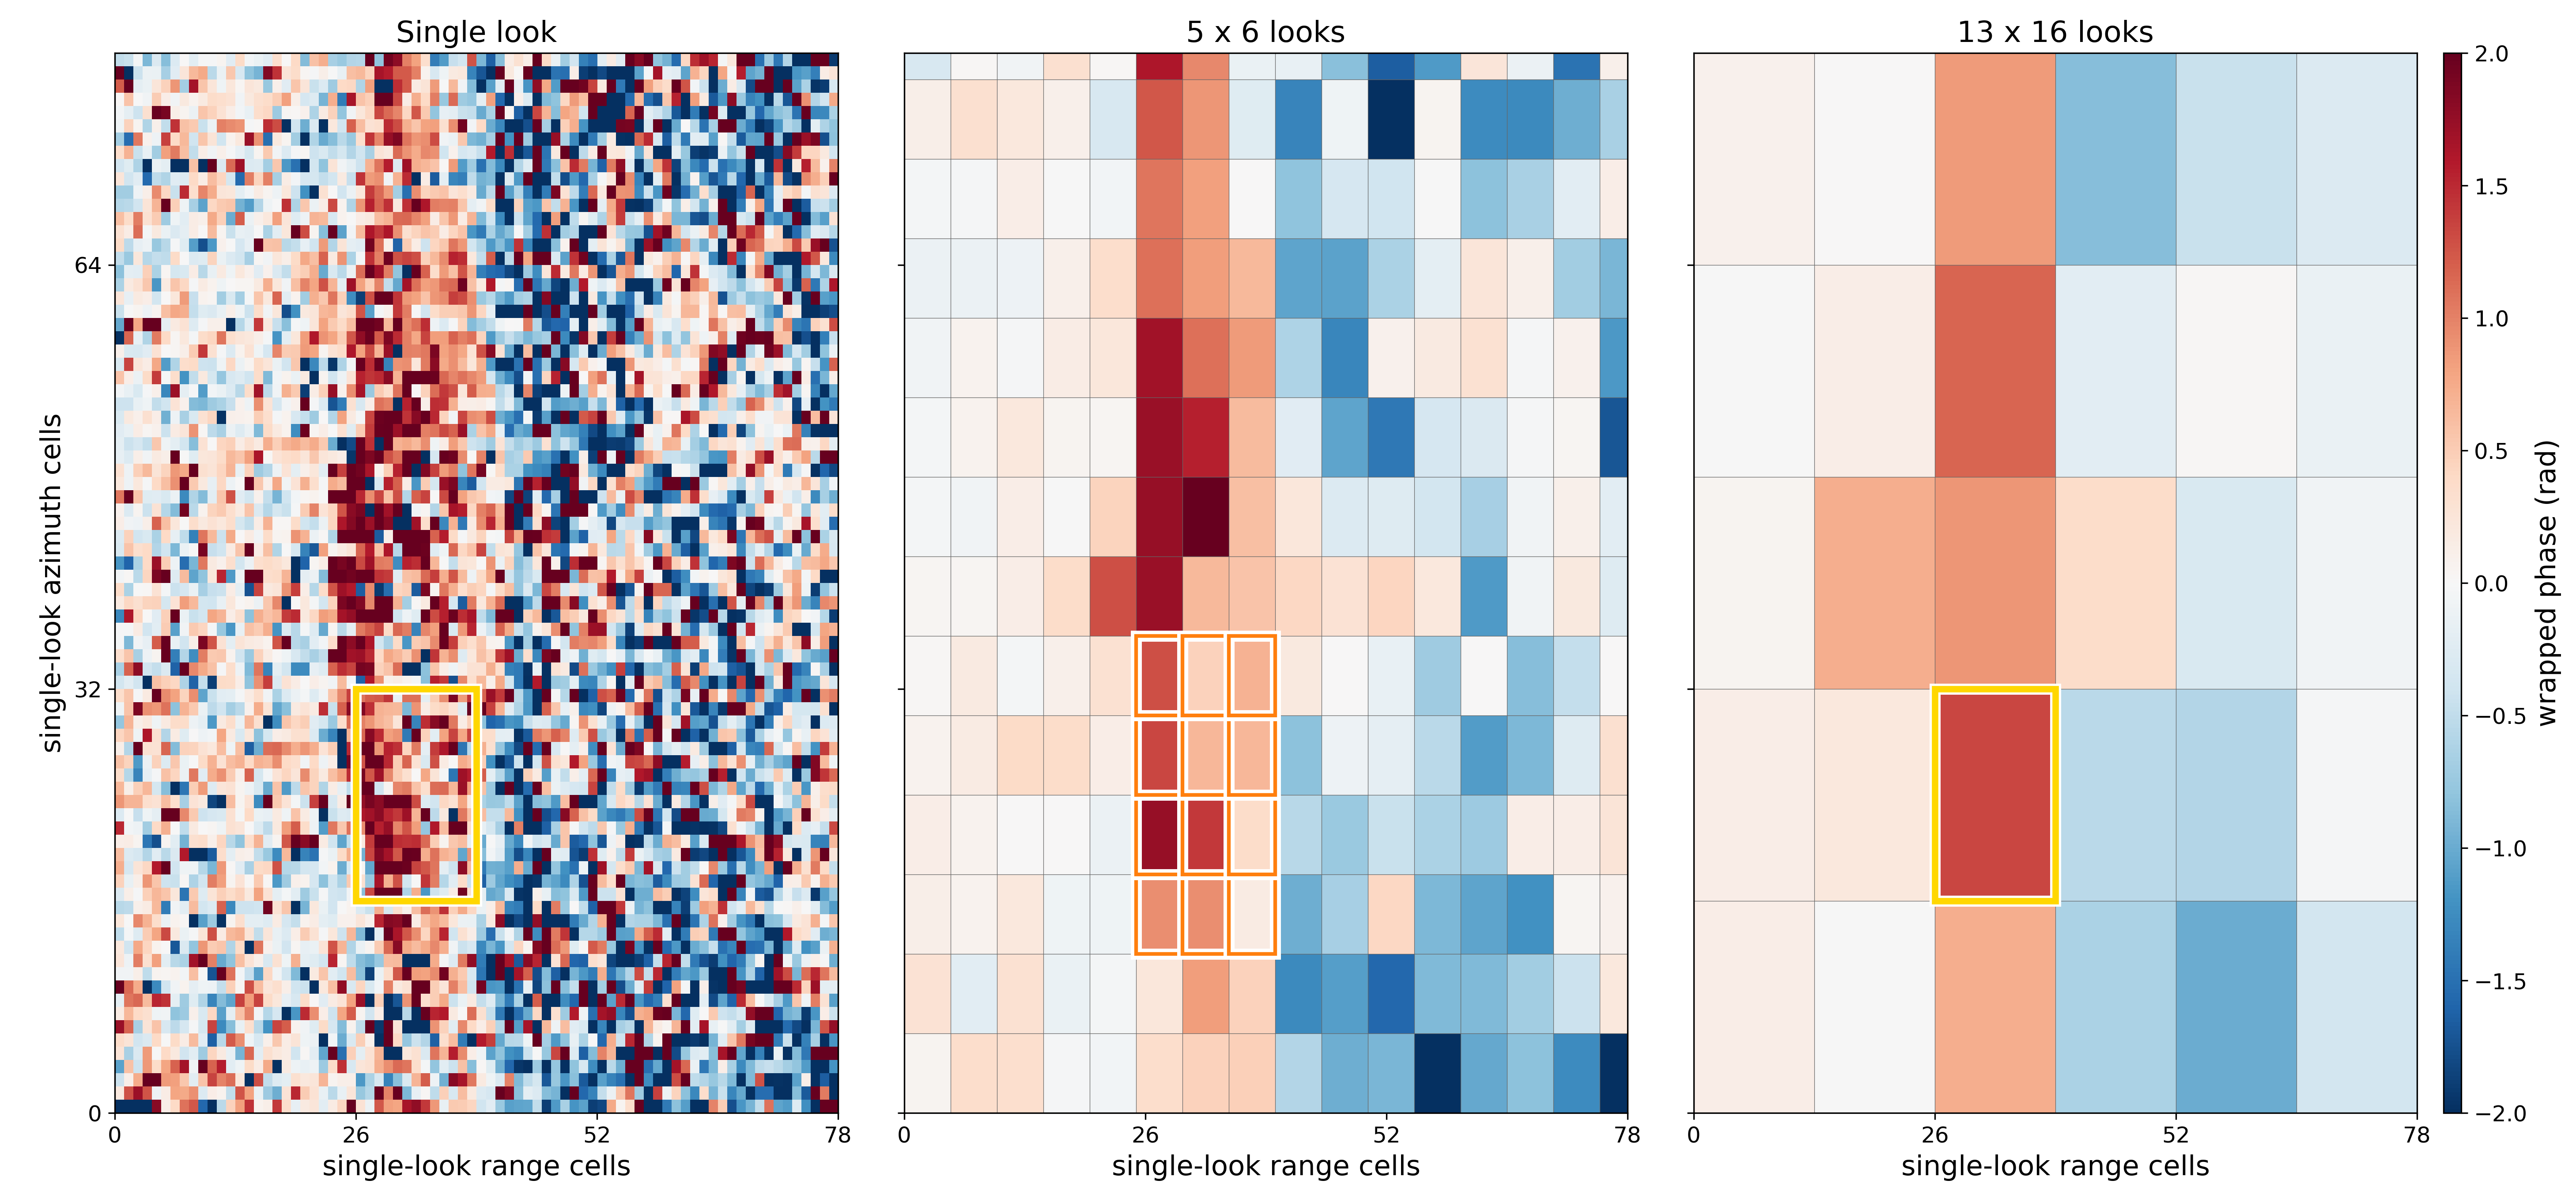
\includegraphics[width=1.0\linewidth]{figures/0_multilook_windows.png}
    \caption{\DIFaddFL{One NISAR interferogram at three multi-look window sizes. Wrapped phase of the December 7--19, 2025 pair over a 245$\times$355\,}\unit{m} \DIFaddFL{zoom of the upper Tuolumne basin, in radar coordinates. }\textbf{\DIFaddFL{Left:}} \DIFaddFL{single look resolution cells, $\sim$3\,}\unit{m} \DIFaddFL{slant range resolution by $\sim$7\,}\unit{m} \DIFaddFL{azimuth resolution \mbox{%DIFAUXCMD
\citep{nisar2025handbook}}\hskip0pt%DIFAUXCMD
, sampled at 3.1\,}\unit{m} \DIFaddFL{by 4.5\,}\unit{m}\DIFaddFL{. }\textbf{\DIFaddFL{Center:}} \DIFaddFL{the same zoom multi-looked with the 5$\times$6 cell window of the 20\,}\unit{m} \DIFaddFL{GUNW wrapped-phase layer, each pixel the average of 30 cells. }\textbf{\DIFaddFL{Right:}} \DIFaddFL{the same zoom multi-looked with the 13$\times$16 cell window of the 80\,}\unit{m} \DIFaddFL{GUNW unwrapped-phase layer, each pixel the average of 208 cells. The yellow box marks one 13$\times$16 window and the pixel it becomes, and the orange boxes mark the 20\,}\unit{m} \DIFaddFL{pixels that overlap it.}}
    \label{fig:multilook_windows}
\end{figure}

\DIFadd{The rationale for }\DIFaddend multi-looking \DIFdelbegin \DIFdel{, or performing a complex average of phase over a spatial window, is that it provides a reasonable estimate of what would be measured if many independent observations of the phase could be obtained from the same place and time. This averaging }\DIFdelend \DIFaddbegin \DIFadd{is that it }\DIFaddend reduces phase noise from random scatterers and \DIFaddbegin \DIFadd{other forms of decorrelation and }\DIFaddend improves the estimate of \DIFaddbegin \DIFadd{the complex }\DIFaddend coherence \citep{Zebker1992, Bamler1998}. \DIFaddbegin \DIFadd{For a complex zero-mean Gaussian signal with constant phase across the window, this average is the maximum likelihood estimate of the phase \mbox{%DIFAUXCMD
\citep{Bamler1998}}\hskip0pt%DIFAUXCMD
. }\DIFaddend However, this estimate is only valid under the assumption of stationarity: that every pixel in the window samples the same underlying distribution, with the same mean and variance of phase \DIFdelbegin \DIFdel{. }\DIFdelend \DIFaddbegin \DIFadd{\mbox{%DIFAUXCMD
\citep{Touzi1999, zebker2005accurate-421}}\hskip0pt%DIFAUXCMD
. \mbox{%DIFAUXCMD
\citet{Touzi1999} }\hskip0pt%DIFAUXCMD
relax this to local stationarity, in which the mean phase must not change significantly across the estimation window. }\DIFaddend This assumption is violated when the true $\Delta\mathrm{SWE}$ varies across the multi-look window\DIFdelbegin \DIFdel{causing each pixel's phase PDF to be centered on a different value}\DIFdelend .

To \DIFdelbegin \DIFdel{show this effect, we first model the phase $\phi (x)$ of each single-look-complex (SLC) }\DIFdelend \DIFaddbegin \DIFadd{separate the phase of the window-mean $\Delta\mathrm{SWE}$ from the variation of $\Delta\mathrm{SWE}$ among the cells, we write the phase $\Delta\phi(x)$ of each single-look }\DIFaddend resolution cell $x$ \DIFdelbegin \DIFdel{within a spatial }\DIFdelend \DIFaddbegin \DIFadd{in a }\DIFaddend multi-look window as 
\DIFdelbegin \DIFdel{the phase of the window-mean $\Delta\mathrm{SWE}$ ($\bar{\phi}$) plus a }\DIFdelend \DIFaddbegin 

\begin{equation}\DIFadd{\label{eq:sigma_def}
      \Delta\phi (x) = \underbrace{\overline{\Delta\phi}}_{\substack{\text{phase of} \\ \text{mean $\Delta\mathrm{SWE}$}}}
           + \underbrace{\delta (x)}_{\substack{\text{per-cell deviation} \\ \text{from mean}}}
}\end{equation}

\noindent \DIFadd{where $\overline{\Delta\phi}$ is the mean phase and  $\delta(x)$ is the }\DIFaddend per-cell deviation\DIFdelbegin \DIFdel{$\delta (x)$. To simplify notation, we use $\phi = \Delta\phi$ for the remainder of this section, and discussions about phase refer to the change in phase between two observations at the same location at different points in time}\DIFdelend . \DIFaddbegin \DIFadd{The deviation is defined by the difference from the window mean, so it sums to zero over the window.
}\DIFaddend 

\DIFdelbegin \begin{displaymath}\DIFdel{\label{eq:sigma_def}
      \phi (x) = \underbrace{\bar{\phi}}_{\substack{\text{phase of} \\ \text{mean $\Delta\mathrm{SWE}$}}}
           + \underbrace{\delta (x)}_{\substack{\text{per-cell deviation} \\ \text{from mean}}}
}\end{displaymath}%DIFAUXCMD
%DIFDELCMD < 

%DIFDELCMD < \noindent %%%
\DIFdel{The observed complex value }\DIFdelend \DIFaddbegin \DIFadd{The noise-free multi-looked estimate of the complex interferogram }\DIFaddend for the window, \DIFaddbegin \DIFadd{$\bar{z}_{\mathrm{window}}$, }\DIFaddend assuming unit amplitude in each cell, is:

\begin{equation}\label{eq:z_window}
    \bar{z}_{\mathrm{window}}
      = \frac{1}{N} \sum_{x=1}^{N} e\DIFdelbegin \DIFdel{^{i\phi(x)}
      }\DIFdelend \DIFaddbegin \DIFadd{^{i\Delta\phi(x)}
      }\DIFaddend \equiv M e\DIFdelbegin \DIFdel{^{i\bar{\phi}}
}\DIFdelend \DIFaddbegin \DIFadd{^{i\overline{\Delta\phi}}
}\DIFaddend \end{equation}

\noindent where \DIFdelbegin \DIFdel{$e^{i\bar{\phi}}$ carries }\DIFdelend \DIFaddbegin \DIFadd{$e^{i\overline{\Delta\phi}}$ governs }\DIFaddend the phase of the window-mean $\Delta\mathrm{SWE}$, and $M$ is a complex factor whose magnitude reflects the spread of the per-cell deviations and whose argument captures the retrieval bias relative to the phase of the window-mean $\Delta\mathrm{SWE}$.

\begin{equation}\label{eq:def_m}
    M = \frac{1}{N} \sum_{x=1}^{N} e^{i\delta(x)}
\end{equation}

\DIFdelbegin \DIFdel{Because $\delta$ }\DIFdelend \DIFaddbegin \DIFadd{Eqs.~(\ref{eq:sigma_def}) to (\ref{eq:def_m}) contain no noise. $\delta(x)$ }\DIFaddend is the deviation \DIFaddbegin \DIFadd{of the true $\Delta\mathrm{SWE}$ phase of cell $x$ }\DIFaddend from the window mean\DIFdelbegin \DIFdel{, it has a zero mean by construction. Stationarity makes its variance spatially constant. Under the stationarity assumption, the SWE-induced noise-free phase is constant }\DIFdelend \DIFaddbegin \DIFadd{. Decorrelation from speckle, temporal change, and thermal noise is treated separately below. If the $\Delta\mathrm{SWE}$ is uniform }\DIFaddend across the window, \DIFdelbegin \DIFdel{so $\delta$ is decorrelation noise alone. We assume our cells are distributed scatterers so the noise is symmetric about the mean and approximately Gaussian at usable coherence. The magnitude $|M|$ is set by the variance of these decorrelation-induced deviations and results in the observed decorrelation.
The symmetry makes the expected $M$ real-valued, so $\arg(M)=0$ and the expected retrieval bias is zero.
}\DIFdelend \DIFaddbegin \DIFadd{the stationary case, then $\delta(x) = 0$ for every cell, $M = 1$, and multi-looking recovers the phase of the window-mean $\Delta\mathrm{SWE}$.
}\DIFaddend 

However, when \DIFdelbegin \DIFdel{cells within the window are drawn from different distributions, $M$ neither leaves the mean phase unbiased nor converges to }\DIFdelend the \DIFdelbegin \DIFdel{ensemble coherence}\DIFdelend \DIFaddbegin \DIFadd{true $\Delta\mathrm{SWE}$ differs from cell to cell within the window, $|M|$ falls below one}\DIFaddend . $\Delta\mathrm{SWE}$ variation across the window centers the per-cell phase distributions on different values, decreasing the length of $M$ and dropping the estimated coherence below the ensemble value. \DIFaddbegin \DIFadd{\mbox{%DIFAUXCMD
\citet{zebker2005accurate-421} }\hskip0pt%DIFAUXCMD
show the same loss for a linear phase ramp, where fringes inside the estimation window lower the estimated correlation by a factor set by the fringe rate. $M$ extends that factor from a ramp to an arbitrary within-window distribution of $\Delta\mathrm{SWE}$. }\DIFaddend If the within-window $\Delta\mathrm{SWE}$ distribution is asymmetric, $M$ also acquires a nonzero argument, rotating the multi-looked phase from the expected phase of the mean $\Delta\mathrm{SWE}$ \citep{fischer1993}.

Figure~\ref{fig:theoretical_example} shows three idealized cases \DIFdelbegin \DIFdel{, with all other decorrelation sources removed, to isolate the effect of in-window }\DIFdelend \DIFaddbegin \DIFadd{of within-window }\DIFaddend $\Delta\mathrm{SWE}$ \DIFdelbegin \DIFdel{variability}\DIFdelend \DIFaddbegin \DIFadd{distributions to illustrate the two effects}\DIFaddend . The three panels differ only in the within-window distribution of $\Delta\mathrm{SWE}$. Multi-looking assumes that the samples in the window share a single phase, \DIFdelbegin \DIFdel{so }\DIFdelend \DIFaddbegin \DIFadd{and }\DIFaddend the constant case (left) is the only one that meets this condition. \DIFdelbegin \DIFdel{Its }\DIFdelend \DIFaddbegin \DIFadd{The window $\Delta\mathrm{SWE}$ }\DIFaddend variance sets the length of the resultant $|M|$ as the phase values from each sample of $\Delta\mathrm{SWE}$ vary (middle and right). \DIFdelbegin \DIFdel{Its skew sets its }\DIFdelend \DIFaddbegin \DIFadd{The $\Delta\mathrm{SWE}$ skew sets the }\DIFaddend rotation $\arg(M)$ as the asymmetric circular distribution rotates the recovered window phase from the phase of the window-mean $\Delta\mathrm{SWE}$ (right).
\DIFdelbegin \DIFdel{Here, we treat all per-cell amplitudes as one, though real backscatter amplitudes vary across the window.
}\DIFdelend 

\begin{figure}
    \centering
    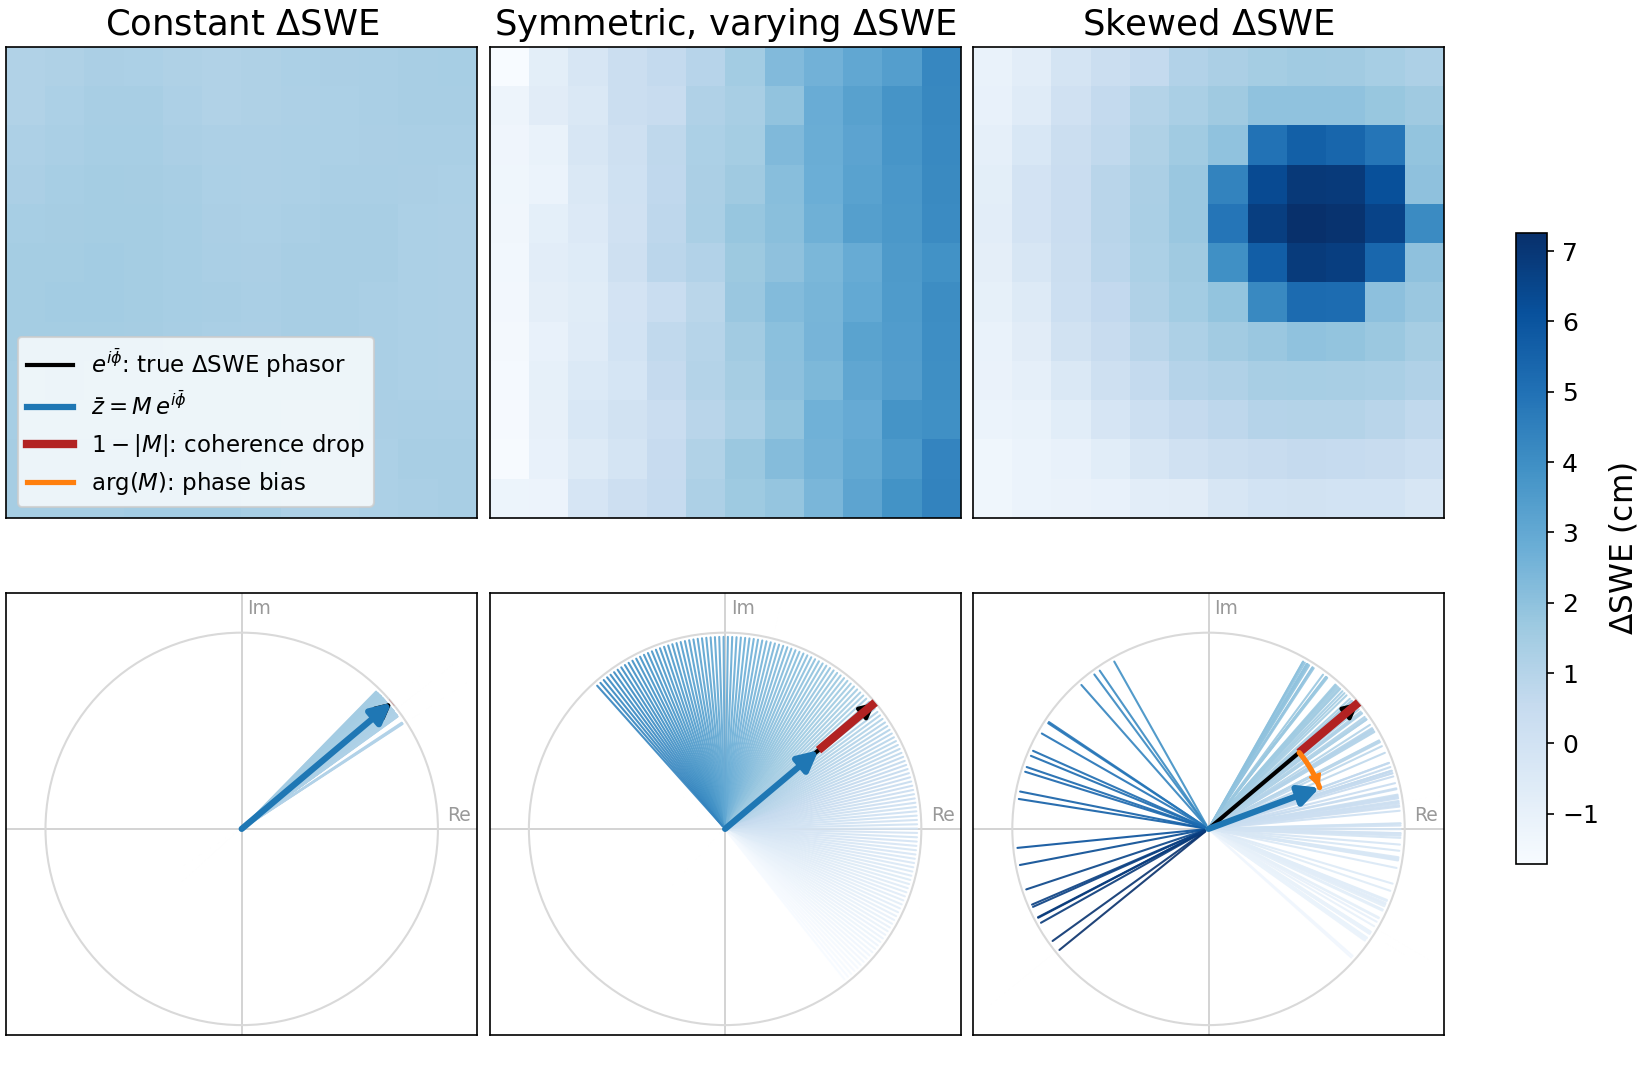
\includegraphics[width=1.0\linewidth]{figures/1_teach_phasor_contrast.png}
    \caption{\DIFdelbeginFL \DIFdelFL{Sub-window }\DIFdelendFL \DIFaddbeginFL \DIFaddFL{Within-window }\DIFaddendFL $\Delta\mathrm{SWE}$ variability and its effect on the multi-looked phasor (all other decorrelation removed). \DIFaddbeginFL \DIFaddFL{Each panel is one multi-look window of 12$\times$12 cells, which becomes one pixel of the product, and each cell in a panel is one single-look resolution cell. The phasors use the L-band $\kappa$ of Section~\ref{subsec:calc-M}. }\DIFaddendFL \textbf{Top:} $\Delta\mathrm{SWE}$ in one window (\unit{cm}), constant (\textbf{left}), varying symmetrically (\textbf{middle}), and skewed (\textbf{right}). \textbf{Bottom:} per-cell unit phasors (\DIFdelbeginFL \DIFdelFL{$\phi=\kappa\Delta\mathrm{SWE}$}\DIFdelendFL \DIFaddbeginFL \DIFaddFL{$\Delta\phi=\kappa\Delta\mathrm{SWE}$}\DIFaddendFL , colored by $\Delta\mathrm{SWE}$). \emph{Black:} mean phasor \DIFdelbeginFL \DIFdelFL{$e^{i\bar\phi}$; }\emph{\DIFdelFL{blue:}} %DIFAUXCMD
\DIFdelendFL \DIFaddbeginFL \DIFaddFL{$e^{i\overline{\Delta\phi}}$. }\emph{\DIFaddFL{Blue:}} \DIFaddendFL resultant \DIFdelbeginFL \DIFdelFL{$\bar z=Me^{i\bar\phi}$; }\emph{\DIFdelFL{red:}} %DIFAUXCMD
\DIFdelendFL \DIFaddbeginFL \DIFaddFL{$\bar z=Me^{i\overline{\Delta\phi}}$. }\emph{\DIFaddFL{Red:}} \DIFaddendFL coherence loss $1-|M|$\DIFdelbeginFL \DIFdelFL{; }\emph{\DIFdelFL{orange arc:}} %DIFAUXCMD
\DIFdelendFL \DIFaddbeginFL \DIFaddFL{. }\emph{\DIFaddFL{Orange arc:}} \DIFaddendFL retrieval bias $\arg(M)$.}
    \label{fig:theoretical_example}
\end{figure}

\DIFdelbegin \DIFdel{The snow-variability coherence loss }\DIFdelend \DIFaddbegin \DIFadd{At L-band and longer wavelengths dry snow is nearly transparent and the return comes from the ground beneath it, so the coherence loss from within-window $\Delta\mathrm{SWE}$ variability }\DIFaddend ($|M|$) \DIFdelbegin \DIFdel{is independent of other decorrelation terms (}\DIFdelend \DIFaddbegin \DIFadd{has a different cause from the within-cell }\DIFaddend temporal, geometric, SNR, \DIFdelbegin \DIFdel{scattering), so it multiplies }\DIFdelend \DIFaddbegin \DIFadd{and scattering terms and multiplies them }\DIFaddend ($\gamma_\mathrm{other}$) to \DIFdelbegin \DIFdel{produce }\DIFdelend \DIFaddbegin \DIFadd{give }\DIFaddend the observed decorrelation (\DIFdelbegin \DIFdel{$\gamma_{\mathrm{obs}}$}\DIFdelend \DIFaddbegin \DIFadd{$\gamma_\mathrm{obs}$}\DIFaddend ):

\begin{equation}\DIFaddbegin \label{eq:gamma_obs}
    \DIFaddend \gamma_\mathrm{obs} = \gamma_\mathrm{other}  |M|
\end{equation}

\noindent \DIFaddbegin \DIFadd{At shorter wavelengths the snow volume itself scatters and changes between passes, and $|M|$ and $\gamma_\mathrm{other}$ are no longer independent.
}

\noindent \DIFaddend $\arg(M)$ is the bias of the \DIFdelbegin \DIFdel{observed }\DIFdelend \DIFaddbegin \DIFadd{multi-looked }\DIFaddend window-mean phase relative to the phase expected from the window-mean $\Delta\mathrm{SWE}$, $\kappa\overline{\Delta\mathrm{SWE}}$. This bias applies even for a perfectly recovered window-mean phase:

\begin{equation}\DIFaddbegin \label{eq:bias}
    \DIFaddend \Delta\phi_\mathrm{obs} = \kappa\overline{\Delta\mathrm{SWE}} + \arg(M)
\end{equation}

\DIFaddbegin \subsection{\DIFadd{Approximate Effect Magnitudes}}\label{subsec:effect-magnitudes}

\DIFadd{Writing $M = |M|\,e^{i\arg(M)}$, the length $|M|$ is the fraction of the phasor amplitude that survives the averaging (the coherence factor) and the angle $\arg(M)$ is the offset of the averaged phase from the phase of the window-mean $\Delta\mathrm{SWE}$ (the retrieval phase bias). Since $M$ is the characteristic function of the within-window distribution of $\delta$, $\log M$ is its cumulant series:
}

\begin{equation}\DIFadd{\label{eq:cumulant_series}
    \log M = \sum_{n \ge 2} \frac{c_n\, i^n}{n!}
           = -\frac{\sigma_\delta^2}{2} - i\,\frac{S\,\sigma_\delta^3}{6} + \dots,
}\end{equation}

\noindent \DIFadd{where the $c_n$ are the cumulants of $\delta$: $c_1 = 0$ because $\delta$ is measured from the window mean, $c_2 = \sigma_\delta^2$ is its variance with $\sigma_\delta = \kappa\,\sigma_{\Delta\mathrm{SWE}}$ and $c_3 = S\sigma_\delta^3$ with $S$ the skewness. Since $\log M = \log|M| + i\arg(M)$, the even terms, which are real, sum to $\log|M|$, and the odd terms, which are imaginary, sum to $\arg(M)$. Keeping the leading term of each,
}

\begin{equation}\DIFadd{\label{eq:cumulant}
    |M| \approx e^{-\kappa^2 \sigma_{\Delta\mathrm{SWE}}^2/2}, \qquad \arg(M) \approx -\frac{S\,\kappa^3 \sigma_{\Delta\mathrm{SWE}}^3}{6}.
}\end{equation}

\noindent \DIFadd{The variance of $\Delta\mathrm{SWE}$ within the window sets the coherence loss and its skew sets the bias. \mbox{%DIFAUXCMD
\citet{Rott2003} }\hskip0pt%DIFAUXCMD
and \mbox{%DIFAUXCMD
\citet{yueh2026interferometric-3ba} }\hskip0pt%DIFAUXCMD
obtain the first term by assuming a Gaussian distribution of $\delta$, which has no odd cumulants and so no bias. Here we keep the bias term as well. At $\sigma_\delta = 1$\,}\unit{rad} \DIFadd{(1.9\,}\unit{cm} \DIFadd{of $\Delta\mathrm{SWE}$ at L-band) the coherence factor is 0.61 and a skewness of one gives $10^\circ$ of bias, and at $\sigma_\delta =1.5$\,}\unit{rad} \DIFadd{(2.8\,}\unit{cm}\DIFadd{) they are 0.32 and $32^\circ$. The series holds while cells stay within about half a fringe of the window mean. Section~\ref{subsec:lidar-variability} compares it with the lidar windows.
}

\DIFaddend Both terms depend only on the within-window distribution of $\Delta\mathrm{SWE}$, so they can be computed from any sufficiently fine $\Delta\mathrm{SWE}$ map. In the following sections, we compute them from lidar-differenced snow surveys and compare against NISAR observed coherences.

\section{Methods}\label{sec:methods}

\subsection{Study Area and Time Frame}\label{subsec:aoi-timeframe}

We target the Tuolumne River basin in the Sierra Nevada (upper Tuolumne and Lyell drainages, 1500--3970\,\unit{m} elevation, $\sim$95$\times$56\,\unit{km}). We use four Airborne Snow Observatory (ASO) lidar pairs bracketing dominant winter accumulations of water years 2023--2026: March 2--16, 2023 (14\,\unit{d}), January 29--February 27, 2024 (29\,\unit{d}), February 8--25, 2025 (17\,\unit{d}), and January 31--February 27, 2026 (27\,\unit{d}). \DIFdelbegin \DIFdel{Pair durations were chosen to }\DIFdelend \DIFaddbegin \DIFadd{Pairs were chosen with temporal separations that }\DIFaddend approximate the NISAR 12-day repeat baseline (one to two repeat cycles per pair) so that the lidar-derived $\Delta\mathrm{SWE}$ is representative of what a single NISAR GUNW would measure. \DIFaddbegin \DIFadd{Figure~\ref{fig:study_area} shows the basin, the lidar coverage, and the NISAR acquisition geometry.
}\DIFaddend 

\DIFaddbegin \begin{figure}
    \centering
    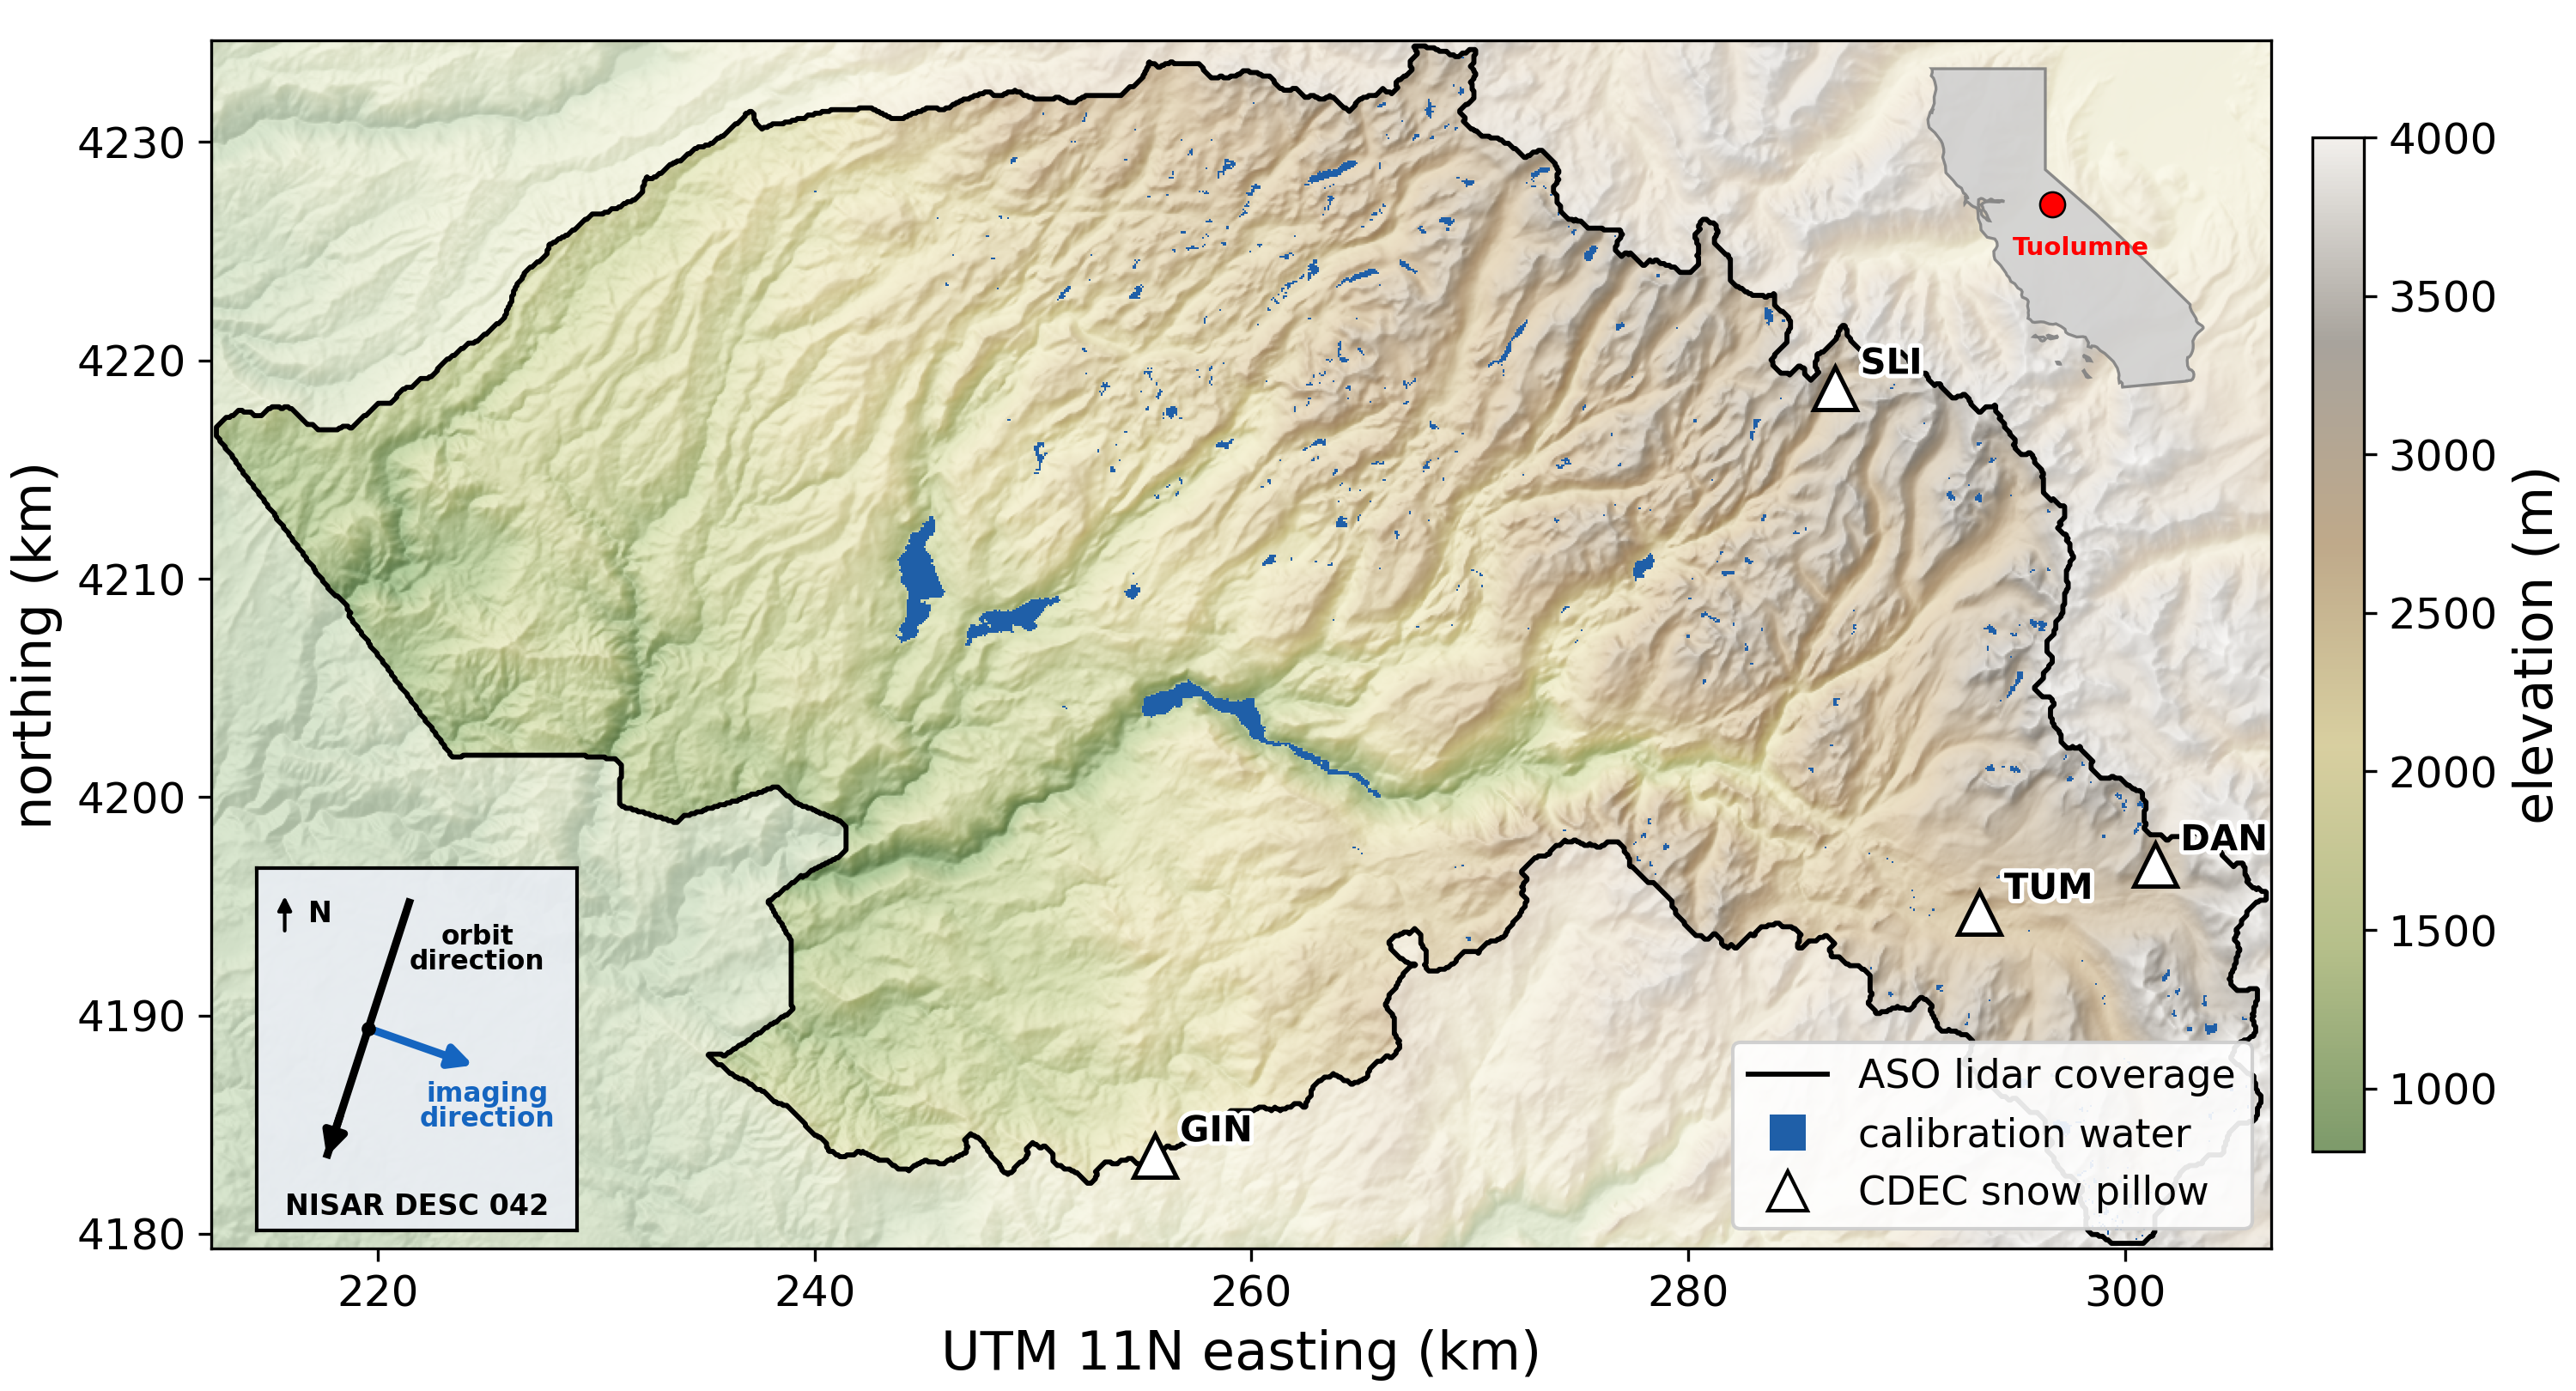
\includegraphics[width=1.0\linewidth]{figures/3_study_area.png}
    \caption{\DIFaddFL{Study area. Elevation with hillshade over the upper Tuolumne basin, with the ASO lidar coverage outlined in black, the water pixels used for the NISAR look calibration (Section~\ref{subsec:nisar-coherence-calc}) in blue, and the four CDEC snow pillows (DAN Dana Meadows, TUM Tuolumne Meadows, SLI Slide Canyon, and GIN Gin Flat). The lower-left inset gives the NISAR flight and imaging directions for the track used.}}
    \label{fig:study_area}
\end{figure}

\DIFaddend For NISAR data, we use \DIFdelbegin \DIFdel{descending track 069, frame 042 }\DIFdelend \DIFaddbegin \DIFadd{the provisional GUNW products (version 1.0.11) from descending track 042, frame 069 }\DIFaddend over the same basin. Three repeat passes on December 7, 19, and 31, 2025 form two consecutive 12-day interferometric pairs. \DIFaddbegin \DIFadd{The perpendicular baselines over the basin are $-109$ and $127$\,}\unit{m} \DIFadd{for the two pairs, giving heights of ambiguity of about 790 and 680\,}\unit{m} \DIFadd{and a geometric decorrelation below 0.005 on flat terrain \mbox{%DIFAUXCMD
\citep{Zebker1992}}\hskip0pt%DIFAUXCMD
. }\DIFaddend No ASO flight pair is coincident with these dates, so we characterize the per-interval snow signal from daily SWE at four Tuolumne-basin CDEC pillows (Dana Meadows, Tuolumne Meadows, Slide Canyon, and Gin Flat). December 7--19 spans a slight ablation window (mean $-1$\,\unit{cm} SWE change), while December 19--31 captures a large December storm (mean $+18$\,\unit{cm} SWE change).

\subsection{Calculation of ASO-$\Delta\mathrm{SWE}$}\label{subsec:aso-phase}

ASO \DIFdelbegin \DIFdel{delivers }\DIFdelend \DIFaddbegin \DIFadd{provides }\DIFaddend snow depth at 3\,\unit{m} \DIFdelbegin \DIFdel{and SWE }\DIFdelend \DIFaddbegin \DIFadd{spatial resolution and SWE, computed from this depth and a modeled snow density, }\DIFaddend at 50\,\unit{m} \DIFdelbegin \DIFdel{, and all }\DIFdelend \DIFaddbegin \DIFadd{spatial resolution \mbox{%DIFAUXCMD
\citep{Deems2013, Painter2016}}\hskip0pt%DIFAUXCMD
. ASO generates snow depths by subtracting gridded snow-off from snow-on surfaces measured by a Riegl scanning lidar with integrated GNSS/IMU positioning \mbox{%DIFAUXCMD
\citep{Deems2013, Painter2016}}\hskip0pt%DIFAUXCMD
. All }\DIFaddend flights for this basin share a common UTM-11N 3\,\unit{m} raster, so pair differencing requires no resampling. For each pair, we form the 3\,\unit{m} $\Delta$depth field $d_B - d_A$ and convert to $\Delta$SWE via a basin-constant new snow density $\rho_\mathrm{event}$ calculated as the pair's mean of per-pixel $\Delta$SWE/$\Delta$depth ratios from the 50\,\unit{m} ASO products, taken over cells where $|\Delta\text{depth}|\geq10$\,\unit{cm} and the implied density lies in $[50, 600]$\,\unit{kg\,m^{-3}}: 304, 312, 373, 330\,\unit{kg\,m^{-3}} for WY2023--2026. Cells where neither flight has $\geq$10\,\unit{cm} of snow at 50\,\unit{m} resolution are masked from the $\Delta$SWE maps. These densities \DIFdelbegin \DIFdel{reflect that the measured snow changes are accumulation with significant settling over the 14--29 day temporal }\DIFdelend \DIFaddbegin \DIFadd{are higher than fresh snow because the accumulation has settled over the 14 to 29 day }\DIFaddend baselines. This approach allows us to take advantage of ASO data with the highest spatial resolution while still centering our analysis on SWE, not snow depth. We block-average the 3\,\unit{m} $\Delta\mathrm{SWE}$ field in non-overlapping 3$\times$3 blocks to \DIFdelbegin \DIFdel{a }\DIFdelend 9\,\unit{m} \DIFdelbegin \DIFdel{pixel size }\DIFdelend \DIFaddbegin \DIFadd{cells }\DIFaddend to suppress any lidar noise (Appendix~\ref{appendix:noise}).

\subsection{\DIFdelbegin \DIFdel{Sub-window }\DIFdelend $\Delta\mathrm{SWE}$ Spectral Structure}\label{subsec:psd}

To identify the spatial scales over which the $\Delta\mathrm{SWE}$ field varies, we compute its radial power spectral density \DIFaddbegin \DIFadd{(Figure~\ref{fig:psd_break}) }\DIFaddend following the snow-depth fractal analyses of \citet{trujillo2007topographic-0ec}. This spatial frequency analysis calculates how $\Delta\mathrm{SWE}$ variance is distributed across spatial scales and tests whether we would expect significant \DIFdelbegin \DIFdel{sub-window }\DIFdelend \DIFaddbegin \DIFadd{within-window }\DIFaddend variability. We test over spatial frequencies from 9 to 380\,\unit{m}. We run the analysis on the native 3\,\unit{m} field rather than the 9\,\unit{m} working grid because the break could fall below the 18\,\unit{m} Nyquist wavelength of the 9\,\unit{m} grid and be unresolvable there. Working on the native 3\,\unit{m} field includes the per-pixel ASO depth noise in the spectrum, which we address in Appendix~\ref{appendix:noise}. A single basin-wide spectrum incorporates many terrain types which blurs any scale breaks, so we work within smaller windows that span a narrower range of elevation, terrain roughness, and vegetation, the topographic and canopy properties shown to control snow-depth scaling. We tile the common snow mask (cells with valid $\Delta\mathrm{SWE}$ in all four pairs) into non-overlapping 1.15\,\unit{km} windows (384 cells on a side) on the native 3\,\unit{m} grid and keep windows \DIFdelbegin \DIFdel{that are }\DIFdelend \DIFaddbegin \DIFadd{in which }\DIFaddend at least 95\% \DIFdelbegin \DIFdel{snow-covered}\DIFdelend \DIFaddbegin \DIFadd{of the 3\,}\unit{m} \DIFadd{cells pass the lidar snow mask of Section~\ref{subsec:aso-phase} in all four pairs}\DIFaddend . This window size holds three full cycles of the longest fitted wavelength (380\,\unit{m}) while staying small enough to remain approximately locally homogeneous. Within the retained windows, any invalid cells (at most 5\% of a window) are filled with the window mean. For each window and each ASO pair, we remove the window mean, apply a Hann taper, and form the two-dimensional periodogram as a function of spatial wavenumber $k$ (\unit{cycles\,m^{-1}}) \citep{harris1978use-0d1}. We apply no higher-order detrend beyond this mean removal because subtracting a planar trend suppresses the longest-wavelength power and biases the large-scale slope \citep{deems2006}.

The four ASO pairs span an order of magnitude in mean $\Delta\mathrm{SWE}$, so a direct average of their spectra would be dominated by the largest-accumulation pair. We instead amplitude-normalize each window's spectrum, subtracting its mean log power over the fitted power spectral density wavelength range of 9 to 380\,\unit{m} before averaging the four pairs' log spectra, which isolates the shared spectral shape. We fit each window's mean spectrum with a continuous two-segment power law, $P(k)\propto k^{-\beta}$, using linear least squares in log--log space weighted by the number of frequencies sampled in each radial bin. The innermost radial bins average only a few frequencies each, so in an unweighted fit, these few noisy values would control the large-scale slope. The scale break is optimized over spatial wavelengths $\ell=1/k$ from 12 to 250\,\unit{m}, and the break wavelength $\ell_b$ is where the small-scale and large-scale regimes meet. We record a small-scale slope, a large-scale slope, and $\ell_b$ for each window. We also fit each pair separately to test whether the break is consistent across the four winters.

\subsection{Calculation of $M$}\label{subsec:calc-M}

For each ASO-derived $\Delta\mathrm{SWE}$ field, we compute the complex \DIFdelbegin \DIFdel{sub-window }\DIFdelend factor $M$ defined in Section~\ref{sec:theoretical-framework}. All processing steps in this section work on a common grid in UTM zone 11N (EPSG:32611) with the origin (upper-left corner) at x = 212352\,\unit{m}, y = 4234641\,\unit{m}.

The $\Delta\mathrm{SWE}$ map for each ASO pair is converted to $\Delta\phi$ \DIFdelbegin \DIFdel{using }\DIFdelend \DIFaddbegin \DIFadd{with the dry-snow approximation of \mbox{%DIFAUXCMD
\citet{Leinss2015}}\hskip0pt%DIFAUXCMD
,
}

\begin{equation}\DIFadd{\label{eq:kappa}
    \kappa(\theta,\lambda) = \frac{2\pi}{\lambda}\left(1.59 + \theta^{5/2}\right),
}\end{equation}

\noindent \DIFadd{with $\theta$ in radians, which for }\DIFaddend NISAR's central frequency (1.26\,\unit{GHz}\DIFaddbegin \DIFadd{, $\lambda = 23.8$\,}\unit{cm}\DIFadd{, \mbox{%DIFAUXCMD
\citealp{nisar2025handbook}}\hskip0pt%DIFAUXCMD
}\DIFaddend ) and a 40$^{\circ}$ local incidence angle \DIFdelbegin \DIFdel{, giving a $\kappa$ of 52.7}\DIFdelend \DIFaddbegin \DIFadd{gives $\kappa = 52.7$}\DIFaddend \,\unit{rad\,m^{-1}} of $\Delta\mathrm{SWE}$\DIFdelbegin \DIFdel{, then wrapped onto ($-\pi$, $\pi$)}\DIFdelend \DIFaddbegin \DIFadd{. We multiply the ASO $\Delta\mathrm{SWE}$ maps by $\kappa$ to generate the expected phase changes, then wrap them onto $(-\pi, \pi]$}\DIFaddend . The 40$^{\circ}$ local incidence angle is chosen to represent a moderate incidence angle across NISAR's typical range, but we note that $\kappa$ is sensitive to this choice \citep{Leinss2015}. \DIFaddbegin \DIFadd{Because $\theta$ is held fixed for every cell, the $|M|$ and $\arg(M)$ reported here isolate the effect of $\Delta\mathrm{SWE}$ variability alone. Any within-window variation of the local incidence angle over real terrain, which changes $\kappa$ from cell to cell, is excluded.
}\DIFaddend 

We then form the complex variability factor $M$ from non-overlapping $9\times9$-pixel (81\,\unit{m}) windows of \DIFaddbegin \DIFadd{ASO-derived }\DIFaddend $\Delta\phi$\DIFdelbegin \DIFdel{, approximately matching the 80\,}%DIFDELCMD < \unit{m} %%%
\DIFdel{GUNW posting}\DIFdelend :

\begin{equation}\label{eq:calc_m}
    M = \frac{1}{N}\sum_{n=1}^{N} e^{i(\Delta\phi_n - \overline{\Delta\phi})},
\end{equation}

where $\Delta\phi_n = \kappa\Delta\mathrm{SWE}_n$, $\overline{\Delta\phi} = \kappa\,\overline{\Delta\mathrm{SWE}}$, $\overline{\Delta\mathrm{SWE}}$ is the mean $\Delta\mathrm{SWE}$ in the window, and $N$ is the number of snow-covered pixels in the window. This is the theoretical Eq.~(\ref{eq:def_m}) reformulated to incorporate the mean ASO $\Delta\mathrm{SWE}$ within the window. We retain $|M|$ and $\arg(M)$ \DIFdelbegin \DIFdel{for windows with $N \geq 41$ (at least half of the }\DIFdelend \DIFaddbegin \DIFadd{only for windows in which at least 41 of the 81 }\DIFaddend pixels are snow-covered\DIFdelbegin \DIFdel{).
}\DIFdelend \DIFaddbegin \DIFadd{, defined as lidar snow depth of at least 0.1\,}\unit{m} \DIFadd{in either ASO flight (Section~\ref{subsec:aso-phase}). NISAR multi-looks in radar coordinates, so its 13$\times$16 cell window covers about 58 by 71\,}\unit{m} \DIFadd{on the ground at the basin's 45$^\circ$ incidence angle before the product is geocoded to its 80\,}\unit{m} \DIFadd{posting, and its 5$\times$6 cell window about 22 by 27\,}\unit{m}\DIFadd{. We use square 81\,}\unit{m} \DIFadd{windows here, and 21\,}\unit{m} \DIFadd{windows in Section~\ref{subsec:sensitivity-of-m-to-window-size}, as close proxies for these two windows.
}\DIFaddend 

We repeat the $M$ calculation at two additional wavelengths: C-band (Sentinel-1, $\lambda = 5.6$\,\unit{cm}) and P-band ($\lambda = 81$\,\unit{cm}). The pipeline is unchanged: the same 9\,\unit{m} pre-averaged $\Delta\mathrm{SWE}$ field and 81\,\unit{m} windows are used, and only $\kappa(\lambda,\theta)$ Eq.~(\DIFdelbegin \DIFdel{\ref{eq:dswe2dphi}}\DIFdelend \DIFaddbegin \DIFadd{\ref{eq:kappa}}\DIFaddend ) is reevaluated for each wavelength, giving $\kappa = 224.1$ and $15.5$\,\unit{rad\,m^{-1}} for C- and P-band, respectively. This produces $|M|$ and $\arg(M)$ maps at 81\,\unit{m} for each band and each ASO pair.

Figure~\ref{fig:phase_wraps_bands} shows the wrapped phase response across 0 to 50\,\unit{cm} of $\Delta\mathrm{SWE}$ at C-, L-, and P-band, with the basin-mean $\pm$ standard deviation of 50\,\unit{m} ASO $\Delta\mathrm{SWE}$ for each pair marked to indicate where each pair sits relative to the wrap interval at each band.

  \begin{figure}
      \centering
      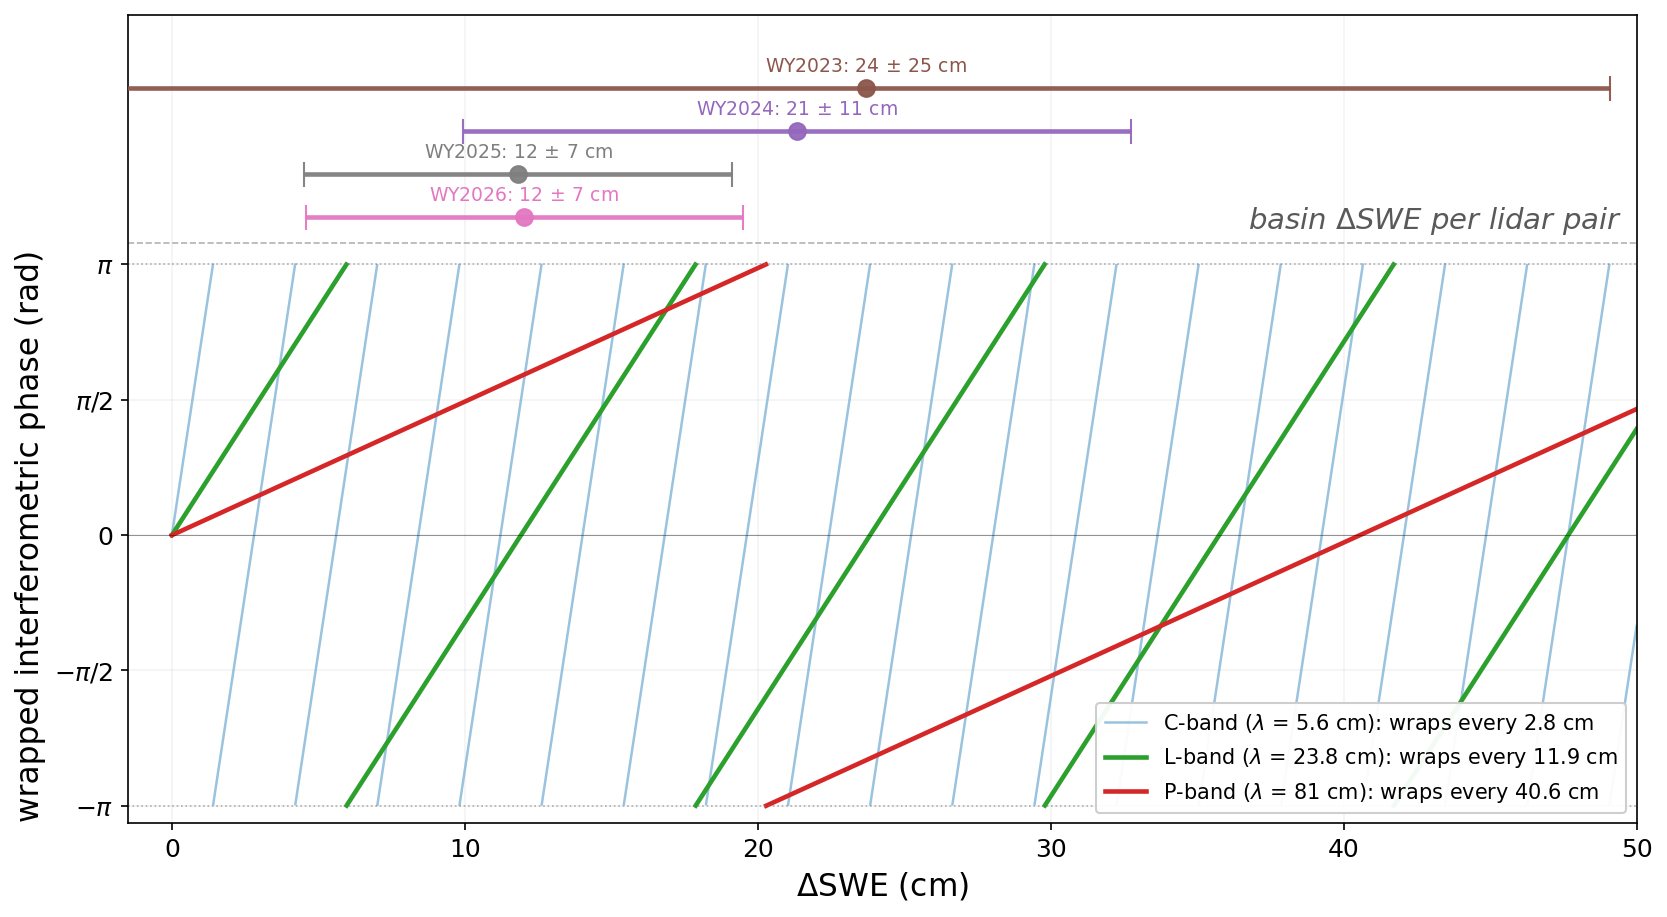
\includegraphics[width=1.0\linewidth]{figures/2_phase_wraps_bands.png}
      \caption{Wrapped interferometric phase response to $\Delta$SWE accumulation 0 to 50\,\unit{cm} at C-band ($\lambda = 5.6$\,\unit{cm}, blue), L-band ($\lambda = 23.8$\,\unit{cm}, green), and P-band ($\lambda = 81$\,\unit{cm}, red), all at $\theta = 40^\circ$ local incidence angle. Each band's phase increases linearly with $\Delta$SWE at the phase rate $\kappa(\lambda, \theta)$ Eq.~(\ref{eq:dswe2dphi}) until it wraps back through $-\pi$. Error bars at the top mark the basin-mean $\Delta$SWE $\pm$ standard deviation for each of the four Tuolumne ASO pairs (50\,\unit{m} basin statistics).}
      \label{fig:phase_wraps_bands}
  \end{figure}

\subsection{Sensitivity of $M$ to Window Size}\label{subsec:sensitivity-of-m-to-window-size}

To trace how the \DIFdelbegin \DIFdel{sub-window }\DIFdelend \DIFaddbegin \DIFadd{within-window }\DIFaddend decorrelation changes with \DIFdelbegin \DIFdel{footprint }\DIFdelend \DIFaddbegin \DIFadd{window }\DIFaddend size, we recompute the window factor $M$ over a range of multi-look window sizes on the 3\,\unit{m} $\Delta\mathrm{SWE}$ field. The window construction follows Section~\ref{subsec:calc-M}. Here the window size is swept from 9 to 81\,\unit{m}, and unlike Section~\ref{subsec:calc-M} the field is not pre-averaged to 9\,\unit{m} so the smaller windows are resolved. The four ASO pairs are restricted to a common snow mask, the per-pixel intersection of their four valid-$\Delta\mathrm{SWE}$ \DIFdelbegin \DIFdel{footprints }\DIFdelend \DIFaddbegin \DIFadd{extents }\DIFaddend on the shared 3\,\unit{m} grid, so each is evaluated over an identical pixel set. We pool the windows across the four pairs at each size and report the median and interquartile range of $|M|$ and of the L-band SWE-equivalent bias $\arg(M)/\kappa$ \DIFaddbegin \DIFadd{(Section~\ref{subsec:effect-magnitudes})}\DIFaddend . The bias is reported only for windows with $|M|>0.3$, since below it $\arg(M)$ is near-uniform over $(-\pi,\pi]$ and carries \DIFdelbegin \DIFdel{no }\DIFdelend \DIFaddbegin \DIFadd{little }\DIFaddend recoverable signal. Working on the native 3\,\unit{m} field folds the per-pixel ASO depth noise into $|M|$, which we address in Appendix~\ref{appendix:noise}.

\subsection{NISAR \DIFdelbegin \DIFdel{Multi-resolution }\DIFdelend Coherence Calculations \DIFaddbegin \DIFadd{Across Window Sizes}\DIFaddend }\label{subsec:nisar-coherence-calc}

The coherence loss due to \DIFdelbegin \DIFdel{sub-window }\DIFdelend \DIFaddbegin \DIFadd{within-window }\DIFaddend $\Delta\mathrm{SWE}$ variability can, in principle, be estimated directly from an interferogram by comparing coherence calculated over different window sizes. The underlying ensemble coherence of a pixel does not depend on the estimation window, but the estimated coherence is affected by two competing, window-size-dependent effects\DIFdelbegin \DIFdel{: }\DIFdelend \DIFaddbegin \DIFadd{. The first is }\DIFaddend a positive bias from estimating coherence magnitude with a finite number of looks, which grows as the window shrinks \citep{Bamler1998}\DIFdelbegin \DIFdel{, and }\DIFdelend \DIFaddbegin \DIFadd{. The second is }\DIFaddend a negative effect from the \DIFdelbegin \DIFdel{sub-window }\DIFdelend \DIFaddbegin \DIFadd{within-window }\DIFaddend variability of the $\Delta\mathrm{SWE}$ signal, assumed in this study to be the dominant source of non-stationarity, which grows as the window expands to span more $\Delta\mathrm{SWE}$ variability. \DIFaddbegin \DIFadd{These are the two biases that \mbox{%DIFAUXCMD
\citet{zebker2005accurate-421} }\hskip0pt%DIFAUXCMD
identify for fringes within the estimation window, and a smaller window is closer to the local stationarity that the sample coherence requires \mbox{%DIFAUXCMD
\citep{Touzi1999}}\hskip0pt%DIFAUXCMD
. }\DIFaddend Because the finite-look bias is analytically known, we can correct each window size and use the remaining coherence difference between window sizes to estimate the potential \DIFdelbegin \DIFdel{sub-window }\DIFdelend \DIFaddbegin \DIFadd{within-window }\DIFaddend $\Delta\mathrm{SWE}$ contribution.

We use the coherence magnitude delivered in each GUNW: the 20\,\unit{m} layer from the wrapped-interferogram group and the 80\,\unit{m} layer from the unwrapped-interferogram group. The expected sample coherence $\hat{\gamma}$ for true coherence $\gamma$ and looks $L$ is given by Eq.~(62) of \citet{Bamler1998}:

\begin{equation}
\mathbb{E}\!\left\{\hat{\gamma}\mid\gamma,L\right\}
= \frac{\Gamma(L)\Gamma\!\left(\tfrac{3}{2}\right)}{\Gamma\!\left(L+\tfrac{1}{2}\right)}\;
{}_{3}F_{2}\!\left(\tfrac{3}{2},L,L;L+\tfrac{1}{2},1;|\gamma|^{2}\right)
\left(1-|\gamma|^{2}\right)^{L},
\label{eq:bamler}
\end{equation}

\noindent where $\Gamma$ is the gamma function and ${}_{3}F_{2}$ is the generalized hypergeometric function. Eq.~(\ref{eq:bamler}) \DIFdelbegin \DIFdel{also assumes circular-Gaussian specklefrom a distributed target, which is a reasonable approximation over snow }\DIFdelend \DIFaddbegin \DIFadd{assumes fully developed speckle, many independent scatterers in every cell, which snow-covered }\DIFaddend and mixed terrain \DIFdelbegin \DIFdel{, but itis a limitation of using this equation}\DIFdelend \DIFaddbegin \DIFadd{approximate well \mbox{%DIFAUXCMD
\citep{zwieback2021repeat-pass-693}}\hskip0pt%DIFAUXCMD
. Cells dominated by a few strong scatterers, such as rock outcrops, depart from it, and the bias correction is only approximate there}\DIFaddend . NISAR multi-looks the full-resolution interferogram in radar coordinates independently for each layer (5$\times$6 for the wrapped layer, 13$\times$16 for the unwrapped layer) and then geocodes each layer onto its delivered map grid \DIFaddbegin \DIFadd{(Figure~\ref{fig:multilook_windows})}\DIFaddend . The geocoding resamples the multi-looked pixels, so neighboring samples on the 20 and 80\,\unit{m} grids are partially correlated, and the nominal look counts ($N = 30$ at 20\,\unit{m}, 208 at 80\,\unit{m}) overstate the number of independent samples. We therefore use an effective look count $L=N/f$, with $f$ an oversampling factor calibrated over \DIFdelbegin \DIFdel{open water on Don Pedro Reservoir near the study site, }\DIFdelend \DIFaddbegin \DIFadd{the permanent water bodies within the study area, chiefly Hetch Hetchy Reservoir, Lake Eleanor, and Cherry Lake, }\DIFaddend where the true coherence is assumed zero at both \DIFdelbegin \DIFdel{resolutions}\DIFdelend \DIFaddbegin \DIFadd{window sizes}\DIFaddend . Water pixels are identified as ESA WorldCover permanent-water (class 80) cells with NISAR 80\,\unit{m} coherence below 0.20, the latter cut removing coherent shoreline pixels. This leaves 13,\DIFdelbegin \DIFdel{189 }\DIFdelend \DIFaddbegin \DIFadd{711 }\DIFaddend open-water samples over the two pairs. Requiring the bias-corrected 20\,\unit{m} and 80\,\unit{m} water coherences to agree gives \DIFdelbegin \DIFdel{$f \approx 1.29$}\DIFdelend \DIFaddbegin \DIFadd{$f \approx 1.32$}\DIFaddend , $L_{20} \approx 23$, and \DIFdelbegin \DIFdel{$L_{80} \approx 162$. }%DIFDELCMD < 

%DIFDELCMD < %%%
\DIFdel{We then de-bias each resolution by inverting }\DIFdelend \DIFaddbegin \DIFadd{$L_{80} \approx 158$. This factor depends on local slope. The ground area of a radar window scales with $1/\sin\theta_\mathrm{loc}$, so on slopes facing the radar one multi-looked window spans more map pixels than on the flat water where $f$ was calibrated, and the effective look count per 80\,}\unit{m} \DIFadd{pixel falls below $N/f$. On slopes facing away it rises. We apply the flat-terrain $f$ everywhere, so the bias correction is approximate on steep terrain.
}

\DIFadd{To correct for the coherence bias, we invert }\DIFaddend Eq.~(\ref{eq:bamler}) \DIFdelbegin \DIFdel{for the true coherence}\DIFdelend \DIFaddbegin \DIFadd{at each window size}\DIFaddend ,

  \begin{equation}
    \tilde{\gamma}_{s} = \mathbb{E}^{-1}\!\left\{\hat{\gamma}_{s}\mid L_{s}\right\},
    \quad s\in\{20,80\},
    \label{eq:debias}
  \end{equation}

\noindent Here \DIFaddbegin \DIFadd{the tilde marks the bias-corrected estimate of the true coherence $\gamma$, which itself remains unknown, and the hat marks the sample coherence delivered in the product. The correction cannot remove the bias entirely. At zero true coherence the expected sample coherence is still positive, so sample values below $\mathbb{E}\{\hat{\gamma}_s \mid \gamma=0, L_s\}$ are clamped to $\tilde{\gamma}_s = 0$. }\DIFaddend $\hat{\gamma}_{20}$ is the 20\,\unit{m} coherence block-averaged onto the 80\,\unit{m} grid before \DIFdelbegin \DIFdel{de-biasing}\DIFdelend \DIFaddbegin \DIFadd{bias correction}\DIFaddend , matching the \DIFdelbegin \DIFdel{footprint }\DIFdelend \DIFaddbegin \DIFadd{window }\DIFaddend on which $f$ was calibrated\DIFdelbegin \DIFdel{; de-biasing }\DIFdelend \DIFaddbegin \DIFadd{. Correcting }\DIFaddend the native 20\,\unit{m} pixels instead would apply $L_{20}$ to samples with fewer effective looks and leaves a small spurious positive residual over zero-coherence water. We then take the difference of the corrected coherences

  \begin{equation}
    \Delta\gamma = \tilde{\gamma}_{20} - \tilde{\gamma}_{80}
    \label{eq:cohdiff}
  \end{equation}

\noindent as our NISAR estimate of the \DIFdelbegin \DIFdel{sub-window-variability coherence loss }\DIFdelend \DIFaddbegin \DIFadd{coherence loss from within-window variability}\DIFaddend . With $\gamma_\mathrm{obs}=|M| \gamma_\mathrm{other}$ and $\tilde\gamma_{20}\approx\gamma_\mathrm{other}$, this difference is $\Delta\gamma \approx \gamma_\mathrm{other}(1-|M|)$, reducing to $1-|M|$ only where the other decorrelation effects are minimal ($\gamma_\mathrm{other} \approx 1$). Because the 20\,\unit{m} reference window already carries some \DIFdelbegin \DIFdel{sub-window }\DIFdelend \DIFaddbegin \DIFadd{within-window }\DIFaddend loss of its own ($|M|_{20}<1$), the difference $\Delta\gamma$ captures only the additional loss incurred between 20 and 80\,\unit{m}, not the full loss relative to a variability-free window. It is therefore a lower bound on the true \DIFdelbegin \DIFdel{sub-window }\DIFdelend \DIFaddbegin \DIFadd{within-window }\DIFaddend coherence loss.

\section{Results}\label{sec:results}

\subsection{$\Delta\mathrm{SWE}$ Power Spectral Densities}\label{subsec:power_spectral_densities}

Resolved per window on the native 3\,\unit{m} grid, the $\Delta\mathrm{SWE}$ spatial power spectrum is a two-regime power law with a break at a median wavelength of $\ell_b = 25$\,\unit{m} (IQR 21--30\,\unit{m} across 572 windows\DIFdelbegin \DIFdel{; }\DIFdelend \DIFaddbegin \DIFadd{, }\DIFaddend Figure~\ref{fig:psd_break}). The spectrum is steep below the break (median slope $\beta = 2.6$) and shallow above it ($\beta = 1.5$): the steep small-scale slope means the $\Delta\mathrm{SWE}$ field is spatially correlated and varies smoothly over separations finer than the $\sim$25\,\unit{m} break, while the shallow large-scale slope means it is rougher and decorrelates over larger separations. Equivalently, the field carries less variance at wavelengths shorter than the break and increasingly more at longer wavelengths. Fitting each ASO pair separately gives $\ell_b$ between 23 and 27\,\unit{m}, and 87\% of the window breaks fall within the 15--40\,\unit{m} range reported for cumulative snow depth \citep{deems2006}.

\begin{figure}
\centering
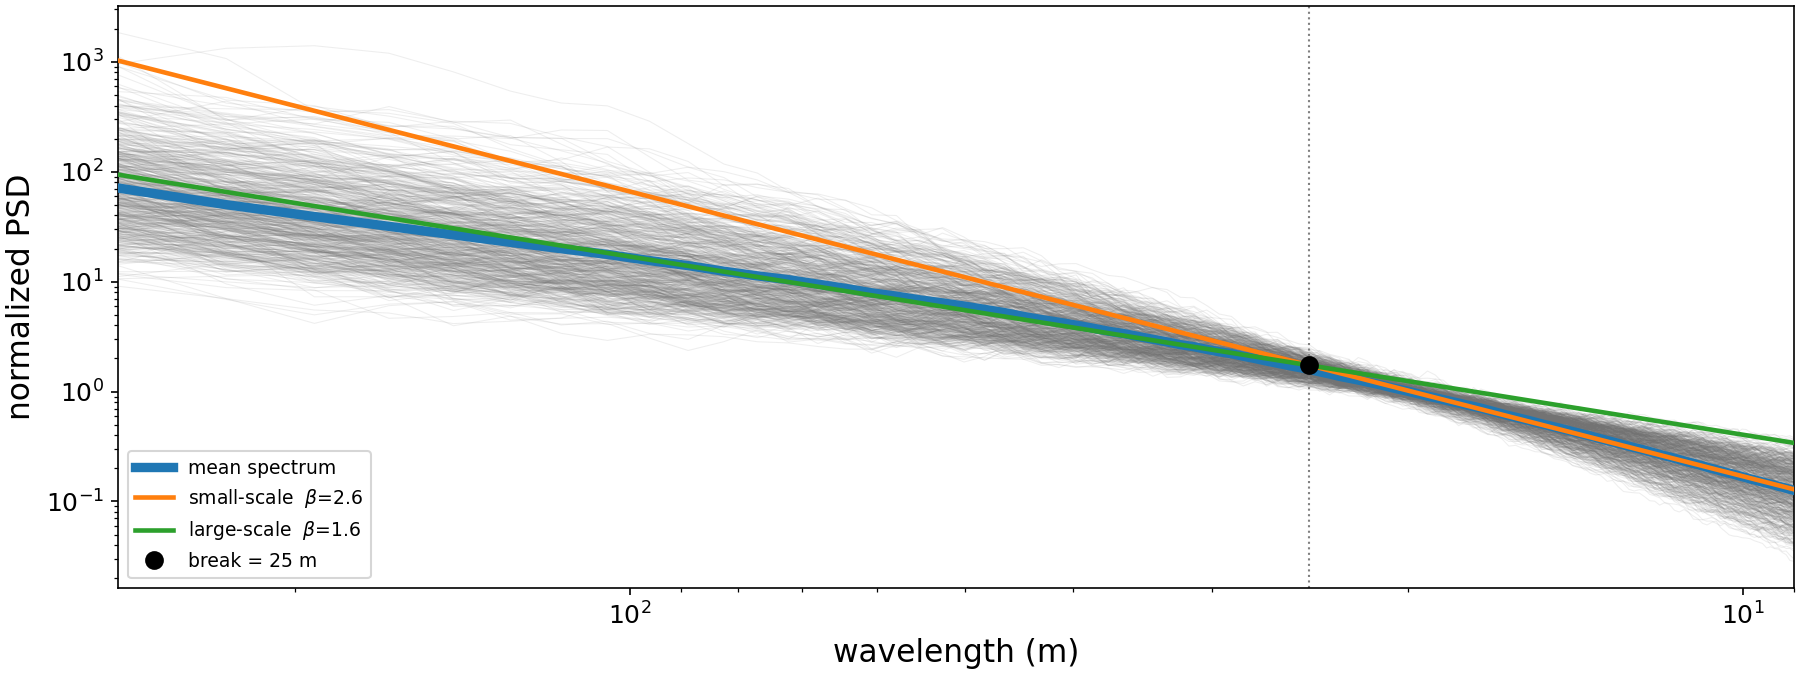
\includegraphics[width=1.0\linewidth]{figures/3_dswe_psd_break.png}
  \caption{Radial power spectral density of the native 3\,\unit{m} $\Delta$SWE field, for each 1.15\,\unit{km} window, amplitude-normalized and averaged over the four lidar pairs so only the spectral shape is compared. Grey lines are the individual windows, blue is their mean, and the orange and green lines are the fitted small-scale and large-scale segments, $P(k)\propto k^{-\beta}$ with $\beta\approx2.6$ and $1.5$. The segments meet at the break (black point) near 25\,\unit{m}.}
  \label{fig:psd_break}
\end{figure}

\subsection{Lidar Derived \DIFdelbegin \DIFdel{Sub-window }\DIFdelend \DIFaddbegin \DIFadd{Within-window }\DIFaddend $\Delta\mathrm{SWE}$ Variability Effects}\label{subsec:lidar-variability}

All lidar $\Delta\mathrm{SWE}$ statistics in this section are computed over the non-overlapping 81\,\unit{m} windows defined in Section~\ref{subsec:calc-M}. Pooled over the four pairs (1.34 million windows), the window-mean $\Delta\mathrm{SWE}$ has a median of 12.6\,\unit{cm} (IQR 4.7--20.4\,\unit{cm}), a \DIFdelbegin \DIFdel{within-window median }\DIFdelend \DIFaddbegin \DIFadd{median within-window }\DIFaddend standard deviation of 3.4\,\unit{cm} (IQR 2.1--6.3\,\unit{cm}) and a slight positive within-window skewness (median $+0.07$, mean $+0.14$). The within-window standard deviation captures the \DIFdelbegin \DIFdel{sub-window }\DIFdelend \DIFaddbegin \DIFadd{within-window }\DIFaddend $\Delta\mathrm{SWE}$ variability that drives $|M|$, and the within-window skew drives $\arg(M)$.

The four pairs show a consistent, terrain-organized spatial pattern. The coherence loss $1-|M|$ and the bias magnitude $|\arg(M)|$ are both largest in the deep, spatially complex alpine terrain and smallest in the smoother, lower-elevation terrain (Figure~\ref{fig:aso_all_pairs}\DIFaddbegin \DIFadd{, elevation in Figure~\ref{fig:study_area}}\DIFaddend ), and both patterns repeat across pairs, with each pair matching the four-pair mean with $r^2=0.75$--$0.82$ for $|M|$ and $0.59$--$0.63$ for $|\arg(M)|$. The sign of the bias is year-specific (signed $\arg(M)$ pairwise $r^2<0.01$)\DIFdelbegin \DIFdel{. Its spatial intensity tracks the }\DIFdelend \DIFaddbegin \DIFadd{, so the bias magnitude follows the }\DIFaddend terrain while its direction varies between events.

Although the basin-median $\Delta\mathrm{SWE}$ ranges over an order of magnitude across the four pairs (0.7--23\,\unit{cm}), the coherence drop and bias stay within narrow bands. Median $|M|$ runs from 0.25 (WY2024) to 0.47 (WY2023\DIFdelbegin \DIFdel{; }\DIFdelend \DIFaddbegin \DIFadd{, }\DIFaddend pooled IQR 0.15--0.58), and the median retrieval bias is near zero ($\leq2^\circ$) with heavy tails (pooled IQR $\pm16^\circ$, widening to $-17^\circ$/$+30^\circ$ in the largest event, WY2024). The three large mid-winter storms (WY2024--2026) drive median $|M|$ to 0.25--0.31, falling to $\sim$0.12--0.16 in the steep high-elevation terrain\DIFdelbegin \DIFdel{, whereas the }\DIFdelend \DIFaddbegin \DIFadd{. The }\DIFaddend pair containing significant melt (WY2023) has the smoothest $\Delta\mathrm{SWE}$ field ($\sigma_{\Delta\mathrm{SWE}}$ median 2.8\,\unit{cm}) \DIFdelbegin \DIFdel{, }\DIFdelend \DIFaddbegin \DIFadd{and }\DIFaddend stays closest to stationarity\DIFdelbegin \DIFdel{, and }\DIFdelend \DIFaddbegin \DIFadd{. It }\DIFaddend shows the highest $|M|$ (0.47) and the least bias (median $\approx0^\circ$). Within WY2023, splitting the windows \DIFdelbegin \DIFdel{by the sign of the window-mean $\Delta\mathrm{SWE}$ }\DIFdelend \DIFaddbegin \DIFadd{into accumulation and melt }\DIFaddend gives a median $|M|$ of 0.55 for melt windows against 0.32 for the accumulation windows\DIFdelbegin \DIFdel{, a gap that persists at matched $|\Delta\mathrm{SWE}|$ magnitude. }\DIFdelend \DIFaddbegin \DIFadd{.
}\DIFaddend 

\begin{figure}
  \centering
  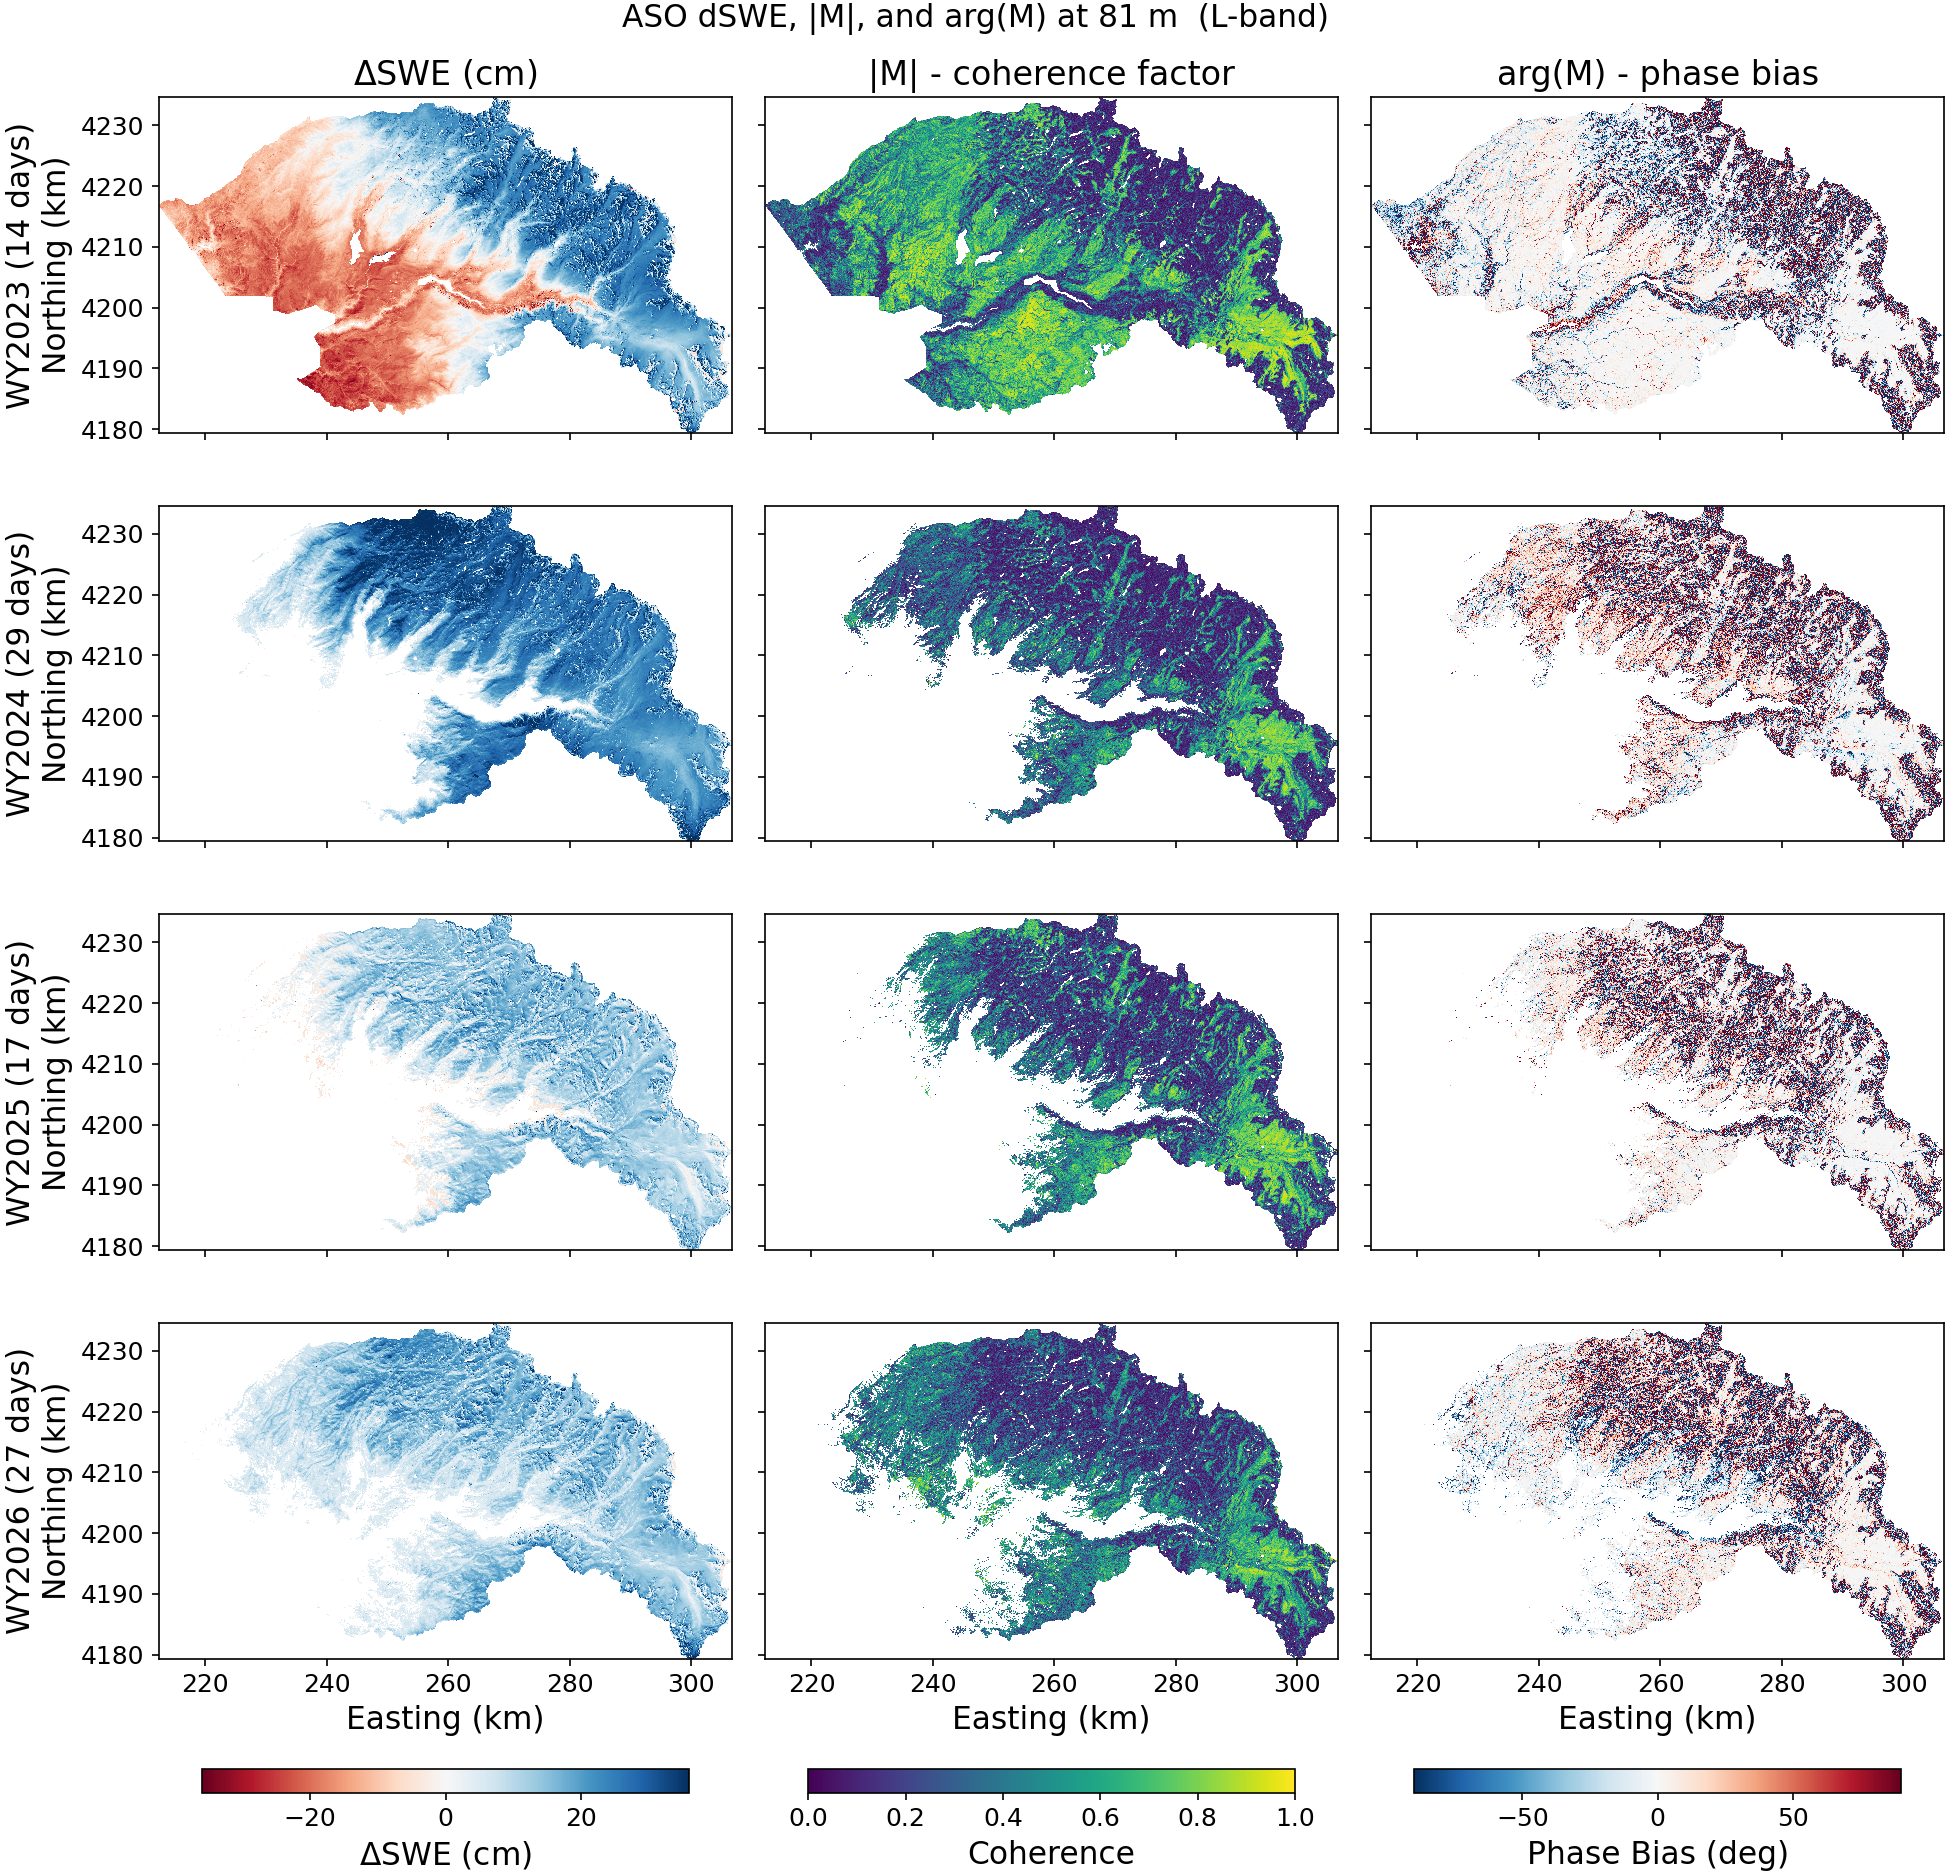
\includegraphics[width=1.0\linewidth]{figures/4_all_pairs_dswe_M_L.png}
  \DIFaddbeginFL \caption{\DIFaddFL{Lidar-derived $\Delta$SWE, coherence factor $|M|$, and retrieval bias $\arg(M)$ at 81\,}\unit{m} \DIFaddFL{for the four Tuolumne lidar pairs (rows, labeled by water year and temporal baseline), evaluated at L-band, 40$^\circ$ local incidence angle. Columns: the 81\,}\unit{m} \DIFaddFL{block-averaged $\Delta$SWE field (}\textbf{\DIFaddFL{left}}\DIFaddFL{), $|M|$ (}\textbf{\DIFaddFL{center}}\DIFaddFL{), and $\arg(M)$ (}\textbf{\DIFaddFL{right}}\DIFaddFL{).}}
  \label{fig:aso_all_pairs}
\end{figure}

\DIFadd{Figure~\ref{fig:M_vs_spread} shows the relationship between the within-window $\Delta\mathrm{SWE}$ variance and the coherence factor and phase bias across the lidar windows, and compares it with the expansion of Section~\ref{subsec:effect-magnitudes}. The Gaussian term reproduces $|M|$ to within 0.05 up to a spread of 1.5\,}\unit{rad} \DIFadd{(2.8\,}\unit{cm} \DIFadd{of $\Delta\mathrm{SWE}$), so the Gaussian assumption is a reasonable estimate of the coherence loss for most windows. Beyond 1.5\,}\unit{rad} \DIFadd{the windows sit above the Gaussian curve, with a median $|M|$ of 0.30 between 1.5 and 2\,}\unit{rad} \DIFadd{against a Gaussian value of 0.22. At large spread the coherence factor settles near 0.1 rather than zero, the magnitude expected from the mean of 81 random unit phasors ($1/\sqrt{N}$), the same finite-sample bias that Eq.~(\ref{eq:bamler}) corrects for the NISAR coherence. The phase bias is minor up to about 1\,}\unit{rad}\DIFadd{, where a skewness of one gives $10^\circ$, and grows quickly beyond it, to $32^\circ$ at 1.5\,}\unit{rad}\DIFadd{. The $S = \pm1$ curves bound the core of the cloud out to that spread. Past it the phase wraps and $M$ depends on the full shape of the distribution rather than on its low moments.
}

\begin{figure}
    \centering
    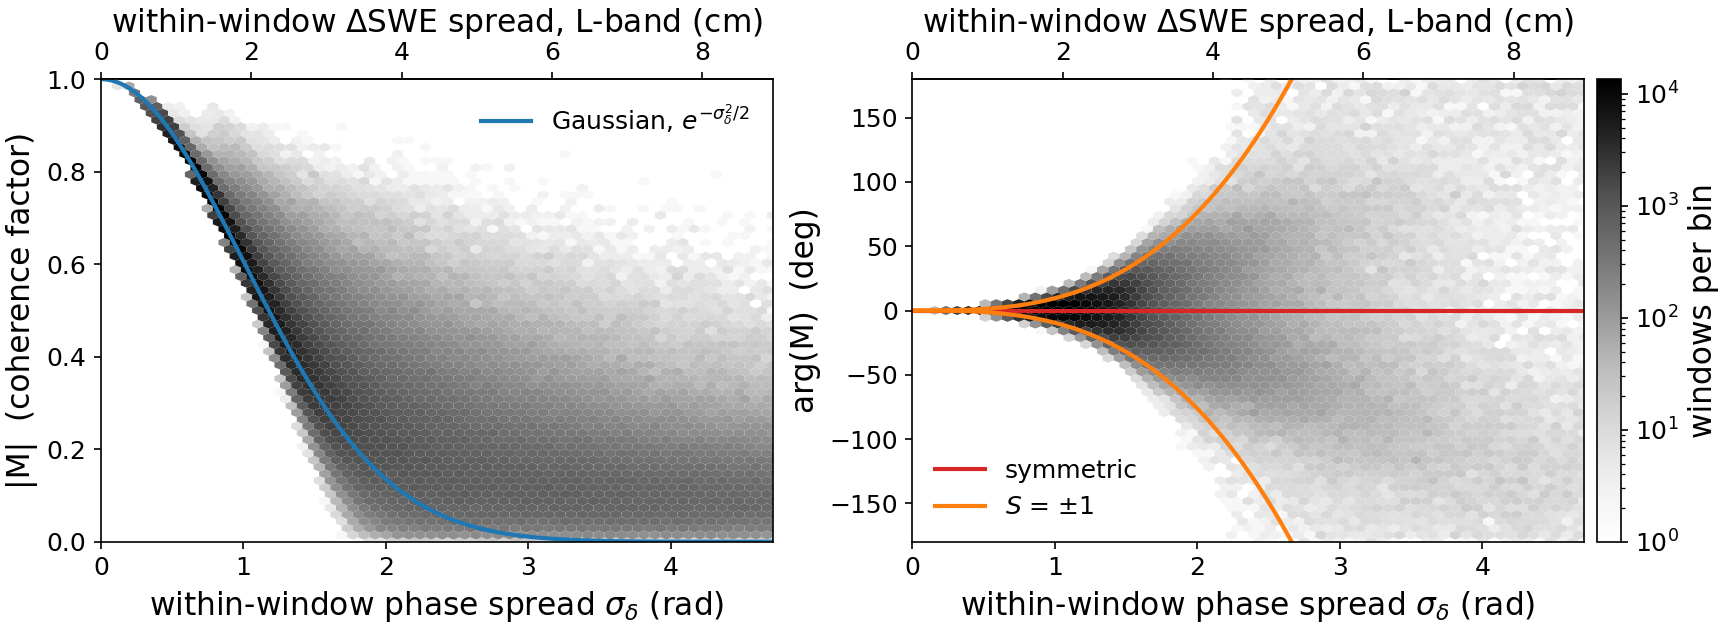
\includegraphics[width=1.0\linewidth]{figures/1b_M_vs_spread.png}
    \DIFaddendFL \caption{\DIFdelbeginFL \DIFdelFL{Lidar-derived $\Delta$SWE, sub-window coherence }\DIFdelendFL \DIFaddbeginFL \DIFaddFL{Coherence }\DIFaddendFL factor $|M|$ \DIFdelbeginFL \DIFdelFL{, }\DIFdelendFL \DIFaddbeginFL \DIFaddFL{(}\textbf{\DIFaddFL{left}}\DIFaddFL{) }\DIFaddendFL and \DIFdelbeginFL \DIFdelFL{retrieval }\DIFdelendFL \DIFaddbeginFL \DIFaddFL{phase }\DIFaddendFL bias $\arg(M)$ \DIFaddbeginFL \DIFaddFL{(}\textbf{\DIFaddFL{right}}\DIFaddFL{) against the within-window phase spread, }\DIFaddendFL at \DIFaddbeginFL \DIFaddFL{the fixed }\DIFaddendFL 81\,\unit{m} \DIFaddbeginFL \DIFaddFL{window size of Section~\ref{subsec:calc-M}, }\DIFaddendFL for \DIFaddbeginFL \DIFaddFL{all lidar windows of }\DIFaddendFL the four \DIFdelbeginFL \DIFdelFL{Tuolumne lidar }\DIFdelendFL pairs (\DIFdelbeginFL \DIFdelFL{rows}\DIFdelendFL \DIFaddbeginFL \DIFaddFL{grey}\DIFaddendFL , \DIFdelbeginFL \DIFdelFL{labeled by water year and temporal baseline}\DIFdelendFL \DIFaddbeginFL \DIFaddFL{logarithmic count}\DIFaddendFL ), \DIFdelbeginFL \DIFdelFL{evaluated at L-band, 40$^\circ$ local incidence angle. Columns: }\DIFdelendFL \DIFaddbeginFL \DIFaddFL{with }\DIFaddendFL the \DIFdelbeginFL \DIFdelFL{81\,}%DIFDELCMD < \unit{m} %%%
\DIFdelFL{block-averaged $\Delta$SWE field }\DIFdelendFL \DIFaddbeginFL \DIFaddFL{leading terms of Eq.~}\DIFaddendFL (\DIFdelbeginFL \textbf{\DIFdelFL{left}}%DIFAUXCMD
\DIFdelendFL \DIFaddbeginFL \DIFaddFL{\ref{eq:cumulant}}\DIFaddendFL ) \DIFdelbeginFL \DIFdelFL{, $|M|$ (}\textbf{\DIFdelFL{center}}%DIFAUXCMD
\DIFdelFL{), }\DIFdelendFL \DIFaddbeginFL \DIFaddFL{for a Gaussian spread }\DIFaddendFL and \DIFdelbeginFL \DIFdelFL{$\arg(M)$ (}\textbf{\DIFdelFL{right}}%DIFAUXCMD
\DIFdelFL{)}\DIFdelendFL \DIFaddbeginFL \DIFaddFL{for a skewness $S$ of $\pm1$}\DIFaddendFL . \DIFaddbeginFL \DIFaddFL{The right panel shows only windows with $|M| > 0.3$.}\DIFaddendFL }
    \DIFdelbeginFL %DIFDELCMD < \label{fig:aso_all_pairs}
%DIFDELCMD < %%%
\DIFdelendFL \DIFaddbeginFL \label{fig:M_vs_spread}
\DIFaddendFL \end{figure}

\subsection{Coherence Loss and Bias Across Window Sizes}\label{subsec:window-size-results}

The L-band coherence factor falls steeply as the multi-look window grows and then plateaus (Figure~\ref{fig:window_size}, left). \DIFaddbegin \DIFadd{Because this sweep runs on the native 3\,}\unit{m} \DIFadd{cells, its absolute level sits below the 9\,}\unit{m} \DIFadd{pipeline of Section~\ref{subsec:lidar-variability} (Appendix~\ref{appendix:noise}), and it is the shape of the curve, not its level, that is compared here. }\DIFaddend The pooled median $|M|$ drops from 0.54 at a 9\,\unit{m} window to 0.33 at 20\,\unit{m} and 0.18 at 81\,\unit{m}, with most of the loss incurred by about 25\,\unit{m}. The interquartile range is wide at every size and stretches further downward as the window grows, spanning 0.07 to 0.38 at 81\,\unit{m}. The two NISAR GUNW \DIFdelbegin \DIFdel{postings }\DIFdelend \DIFaddbegin \DIFadd{window sizes }\DIFaddend bracket a large part of the curve. The 20\,\unit{m} wrapped-interferogram \DIFdelbegin \DIFdel{footprint }\DIFdelend \DIFaddbegin \DIFadd{window }\DIFaddend retains a median $|M|$ of 0.33 compared to 0.18 at the 80\,\unit{m} \DIFdelbegin \DIFdel{footprint}\DIFdelend \DIFaddbegin \DIFadd{window}\DIFaddend , almost double the coherence factor for the same scene.

The L-band retrieval bias stays small across the whole range (Figure~\ref{fig:window_size}, right). In usable windows, the median SWE-equivalent bias never exceeds 0.3\,\unit{mm}, and the interquartile range stays within about $\pm2$\,\unit{mm}. The band is slightly asymmetric, with a longer positive tail (matching the within-window $\Delta\mathrm{SWE}$ skew) but the magnitude is negligible compared to the coherence loss. The bias does not grow significantly at any \DIFdelbegin \DIFdel{footprint }\DIFdelend \DIFaddbegin \DIFadd{window size }\DIFaddend between 9 and 81\,\unit{m}.

\begin{figure}
  \centering
  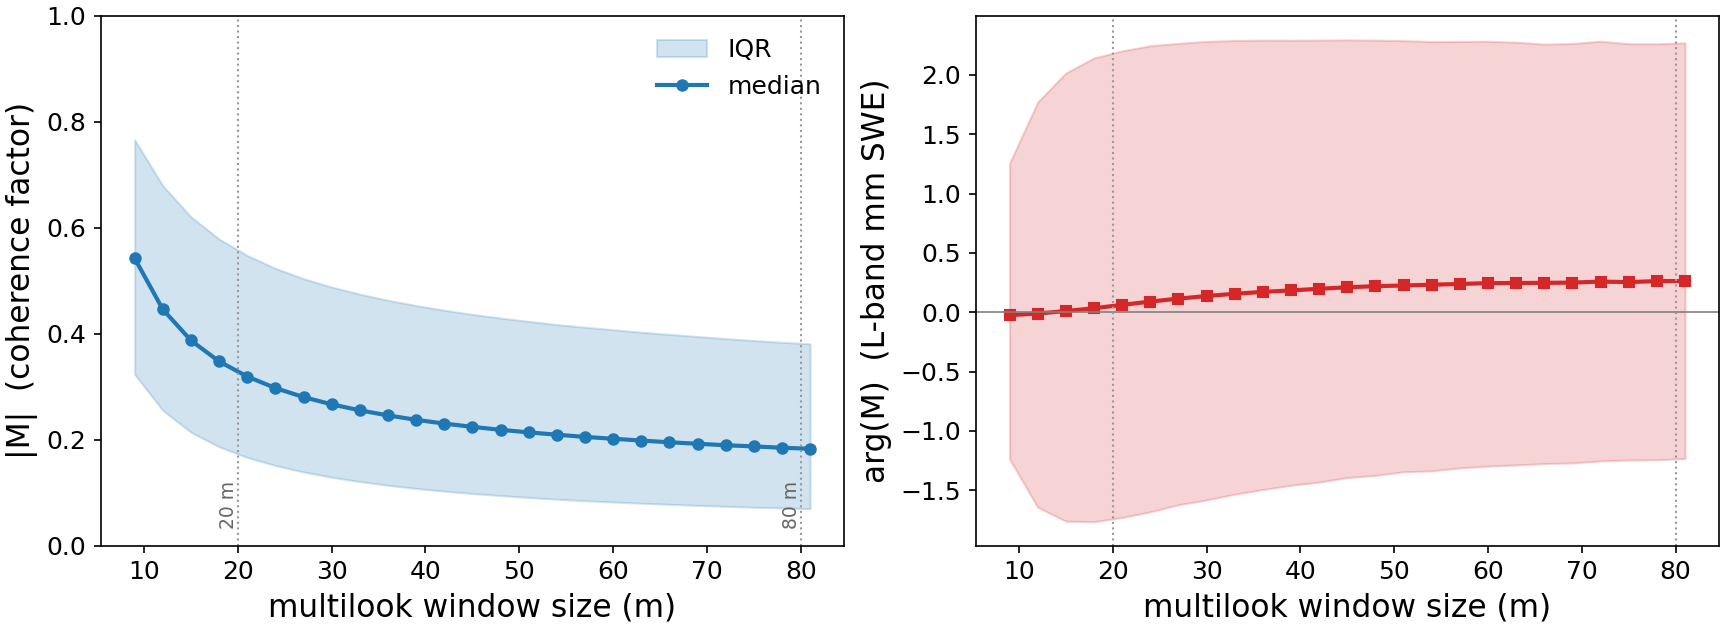
\includegraphics[width=0.8\linewidth]{figures/5_window_M_arg_vs_size_L.png}
  \caption{\DIFdelbeginFL \DIFdelFL{Sub-window coherence }\DIFdelendFL \DIFaddbeginFL \DIFaddFL{Coherence }\DIFaddendFL factor $|M|$ (\textbf{left}) and retrieval bias $\arg(M)$ (\textbf{right}) versus multi-look window size, L-band, pooled over the four lidar pairs (median and shaded interquartile range). Computed on the native 3\,\unit{m} $\Delta\mathrm{SWE}$ field. The right panel is restricted to usable windows ($|M|>0.3$) and converted to an L-band SWE-equivalent through $\arg(M)/\kappa$. Dotted lines mark the 20 and 80\,\unit{m} NISAR GUNW postings.}
  \label{fig:window_size}
\end{figure}


\subsection{NISAR \DIFdelbegin \DIFdel{Multi-resolution }\DIFdelend Coherence \DIFaddbegin \DIFadd{Across Window Sizes}\DIFaddend }\label{subsec:nisar-coherence}

The corrected \DIFdelbegin \DIFdel{$\gamma_{20}-\gamma_{80}$ }\DIFdelend \DIFaddbegin \DIFadd{$\tilde{\gamma}_{20}-\tilde{\gamma}_{80}$ }\DIFaddend is near zero for the near zero-SWE-change December 7--19 pair (median $-0.004$, 45\% of windows positive) and positive for the December 19--31 storm pair (median \DIFdelbegin \DIFdel{$+0.030$, 71}\DIFdelend \DIFaddbegin \DIFadd{$+0.028$, 69}\DIFaddend \% positive) over the snow-covered \DIFdelbegin \DIFdel{footprint }\DIFdelend \DIFaddbegin \DIFadd{extent }\DIFaddend (Figure~\ref{fig:coherence_rows}). Much of the raw $20$--$80$\,\unit{m} gap is finite-look estimation bias. For the December 19--31 pair, the raw gap \DIFdelbegin \DIFdel{$+0.072$ }\DIFdelend \DIFaddbegin \DIFadd{$+0.073$ }\DIFaddend (median) is reduced to \DIFdelbegin \DIFdel{$+0.030$ }\DIFdelend \DIFaddbegin \DIFadd{$+0.028$ }\DIFaddend by the bias correction, while for the \DIFdelbegin \DIFdel{snow-free }\DIFdelend \DIFaddbegin \DIFadd{no-accumulation }\DIFaddend pair, the corrected gap is close to zero. However, the largest corrected residuals cluster at higher elevations, where more $\Delta\mathrm{SWE}$ variability is expected from the lidar. For the storm pair, the corrected gap stays small in the median ($\leq0.04$ across elevations), but its upper tail grows with elevation, with the strongest windows (90th percentile) rising to $\sim$\DIFdelbegin \DIFdel{0.13 }\DIFdelend \DIFaddbegin \DIFadd{0.12 }\DIFaddend in the highest, most exposed terrain, where the 80\,\unit{m} coherence is also lowest (median \DIFdelbegin \DIFdel{0.17}\DIFdelend \DIFaddbegin \DIFadd{0.16}\DIFaddend ).

\begin{figure}
  \centering
  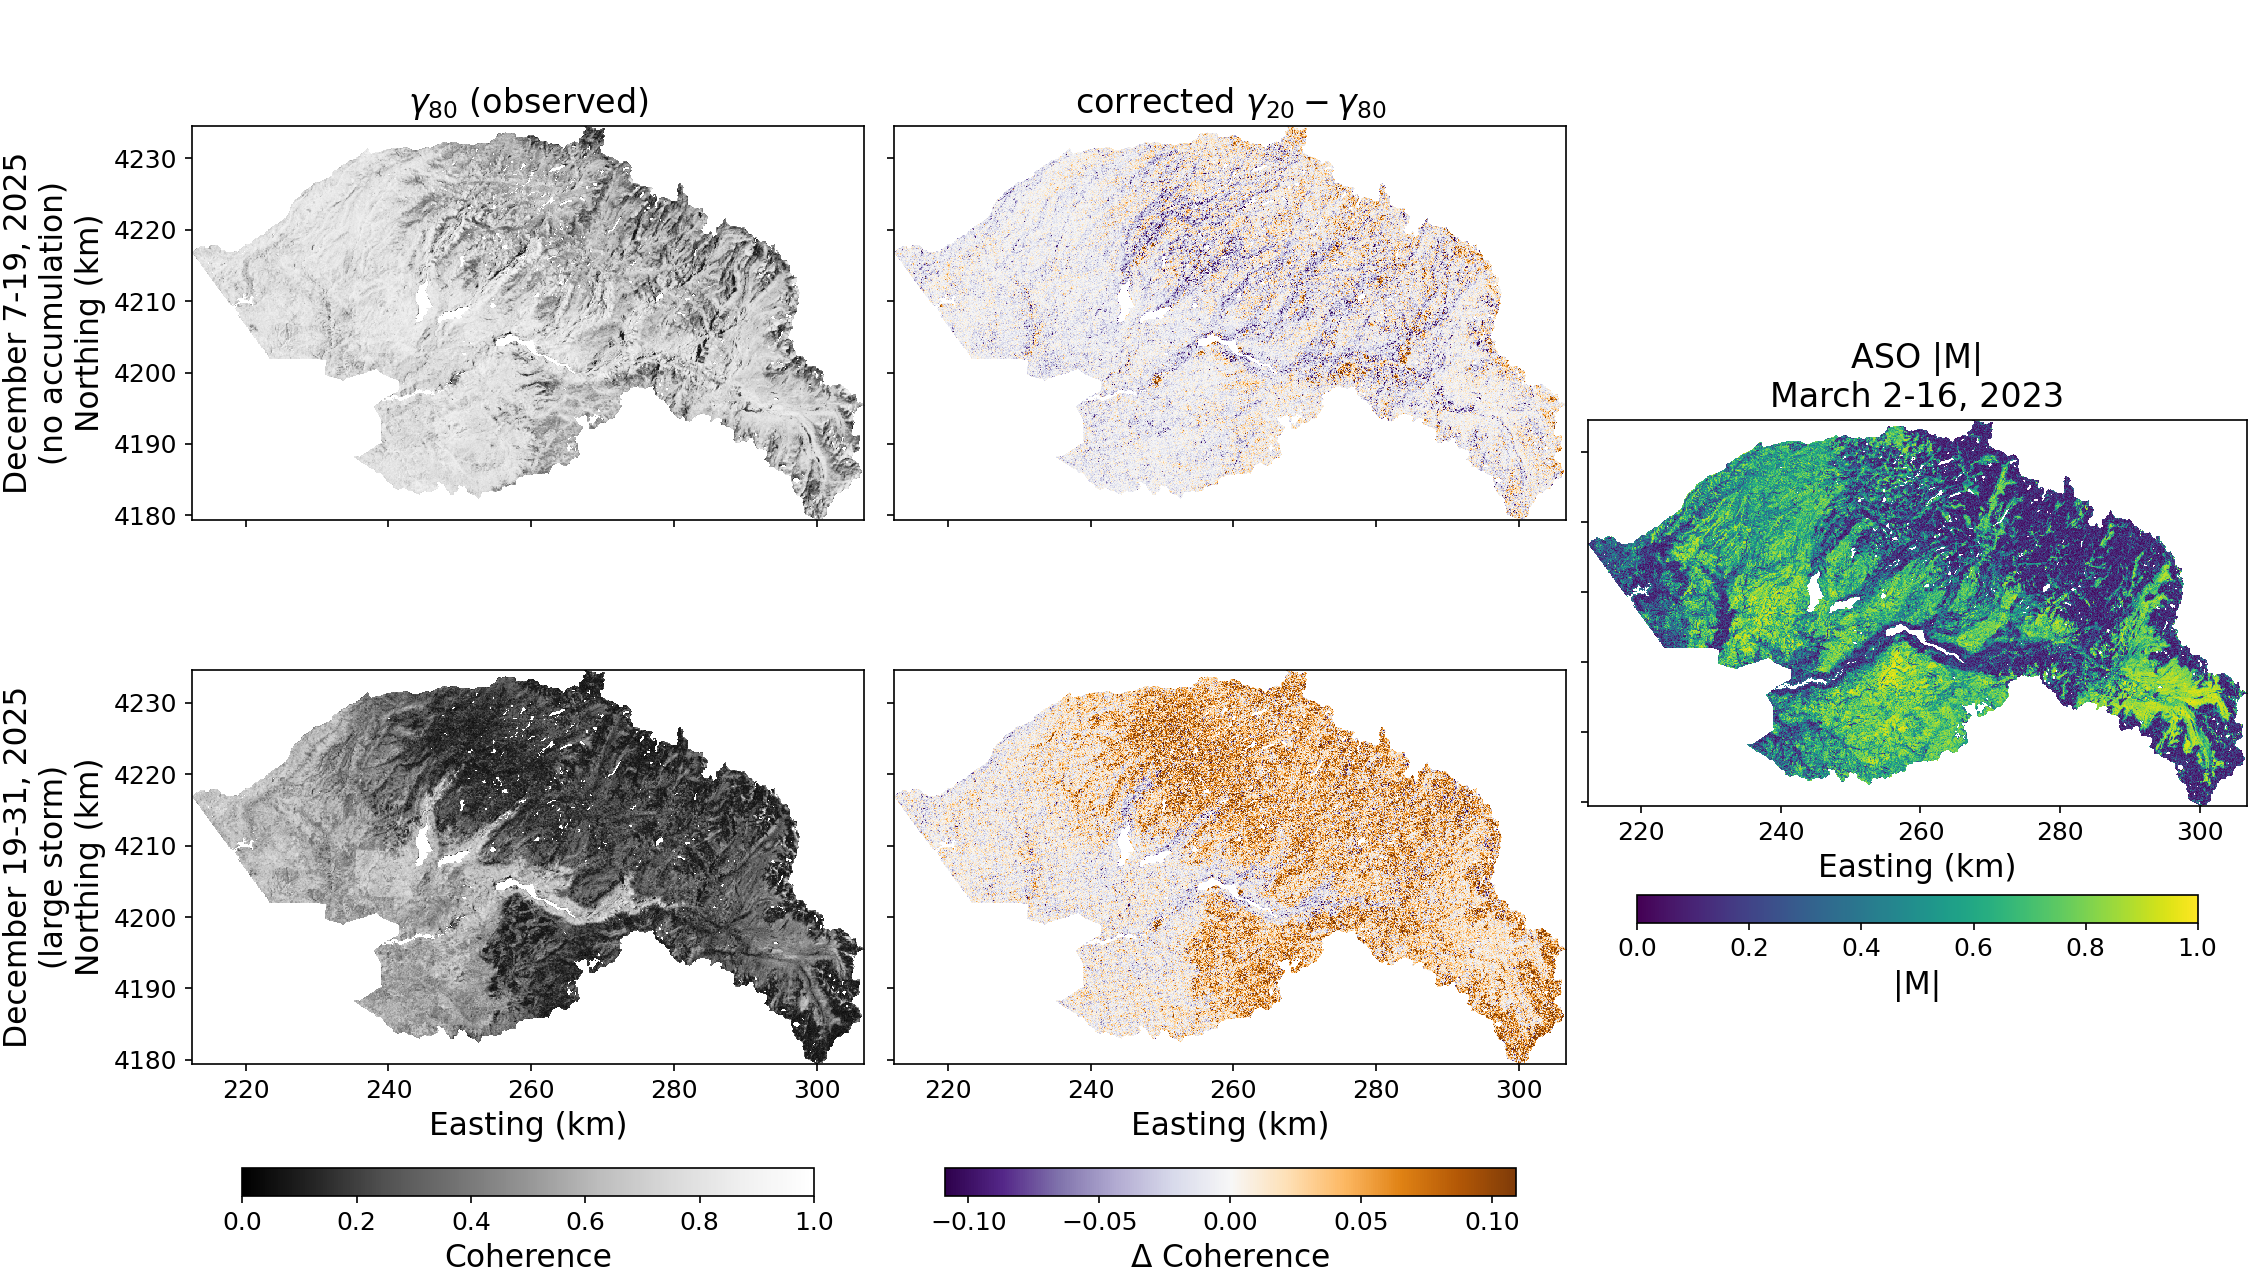
\includegraphics[width=1.0\linewidth]{figures/6_coherence_rows_P12_P23.png}
  \caption{NISAR \DIFdelbeginFL \DIFdelFL{multi-resolution }\DIFdelendFL coherence \DIFaddbeginFL \DIFaddFL{at two window sizes }\DIFaddendFL for the low-snow P12 (December 7--19, 2025) and large-storm P23 (December 19--31, 2025) pairs: observed 80\,\unit{m} coherence \DIFdelbeginFL \DIFdelFL{$\gamma_{80}$ }\DIFdelendFL \DIFaddbeginFL \DIFaddFL{$\hat{\gamma}_{80}$ }\DIFaddendFL (\textbf{left}), the finite-look-corrected difference \DIFdelbeginFL \DIFdelFL{$\gamma_{20}-\gamma_{80}$ }\DIFdelendFL \DIFaddbeginFL \DIFaddFL{$\tilde{\gamma}_{20}-\tilde{\gamma}_{80}$ }\DIFaddendFL (\textbf{center}), and the lidar-predicted \DIFdelbeginFL \DIFdelFL{sub-window }\DIFdelendFL \DIFaddbeginFL \DIFaddFL{within-window }\DIFaddendFL coherence factor $|M|$ (\textbf{right}, WY2023), all on the common 81\,\unit{m} grid.}
  \label{fig:coherence_rows}
\end{figure}

\subsection{Wavelength Effect on $M$}\label{subsec:wavelength-M}

The same \DIFdelbegin \DIFdel{sub-window }\DIFdelend \DIFaddbegin \DIFadd{within-window }\DIFaddend $\Delta\mathrm{SWE}$ field produces very different effects across bands, because shorter wavelengths turn the same $\Delta\mathrm{SWE}$ spread into a larger phase spread and more wrapping (Figure~\ref{fig:M_bands_wy2025}). At C-band ($\kappa = 224.1$\,\unit{rad\,m^{-1}}) the within-window phase spread is large enough that coherence collapses, with median $|M| = 0.10$ (IQR 0.06--0.14) and 53\% of windows below 0.1. So little coherent signal survives that the retrieval bias is undefined, with $\arg(M)$ \DIFdelbegin \DIFdel{distributed nearly uniformly over $\pm90^\circ$, }\DIFdelend \DIFaddbegin \DIFadd{spread over the full circle (}\DIFaddend IQR $-86^\circ$ to $+88^\circ$\DIFaddbegin \DIFadd{)}\DIFaddend . At P-band ($\kappa = 15.5$\,\unit{rad\,m^{-1}}) coherence is largely preserved (median $|M| = 0.87$, IQR 0.65--0.94\DIFdelbegin \DIFdel{; }\DIFdelend \DIFaddbegin \DIFadd{, with }\DIFaddend $<$1\% of windows below 0.1) and the bias is small and well-defined ($\arg(M)$ IQR $-1.6^\circ$ to $+0.3^\circ$). L-band is intermediate, with median $|M| = 0.31$ (IQR 0.15--0.55), 14\% of windows below 0.1, with a small but resolvable bias ($\arg(M)$ IQR $-15^\circ$ to $+19^\circ$). The same ordering holds when \DIFdelbegin \DIFdel{data is }\DIFdelend \DIFaddbegin \DIFadd{the data are }\DIFaddend pooled over all four lidar pairs (median $|M|$ = 0.10 / 0.33 / 0.88 for C/L/P), so that it reflects the wavelength scaling rather than any one event.

\begin{figure}
  \centering
  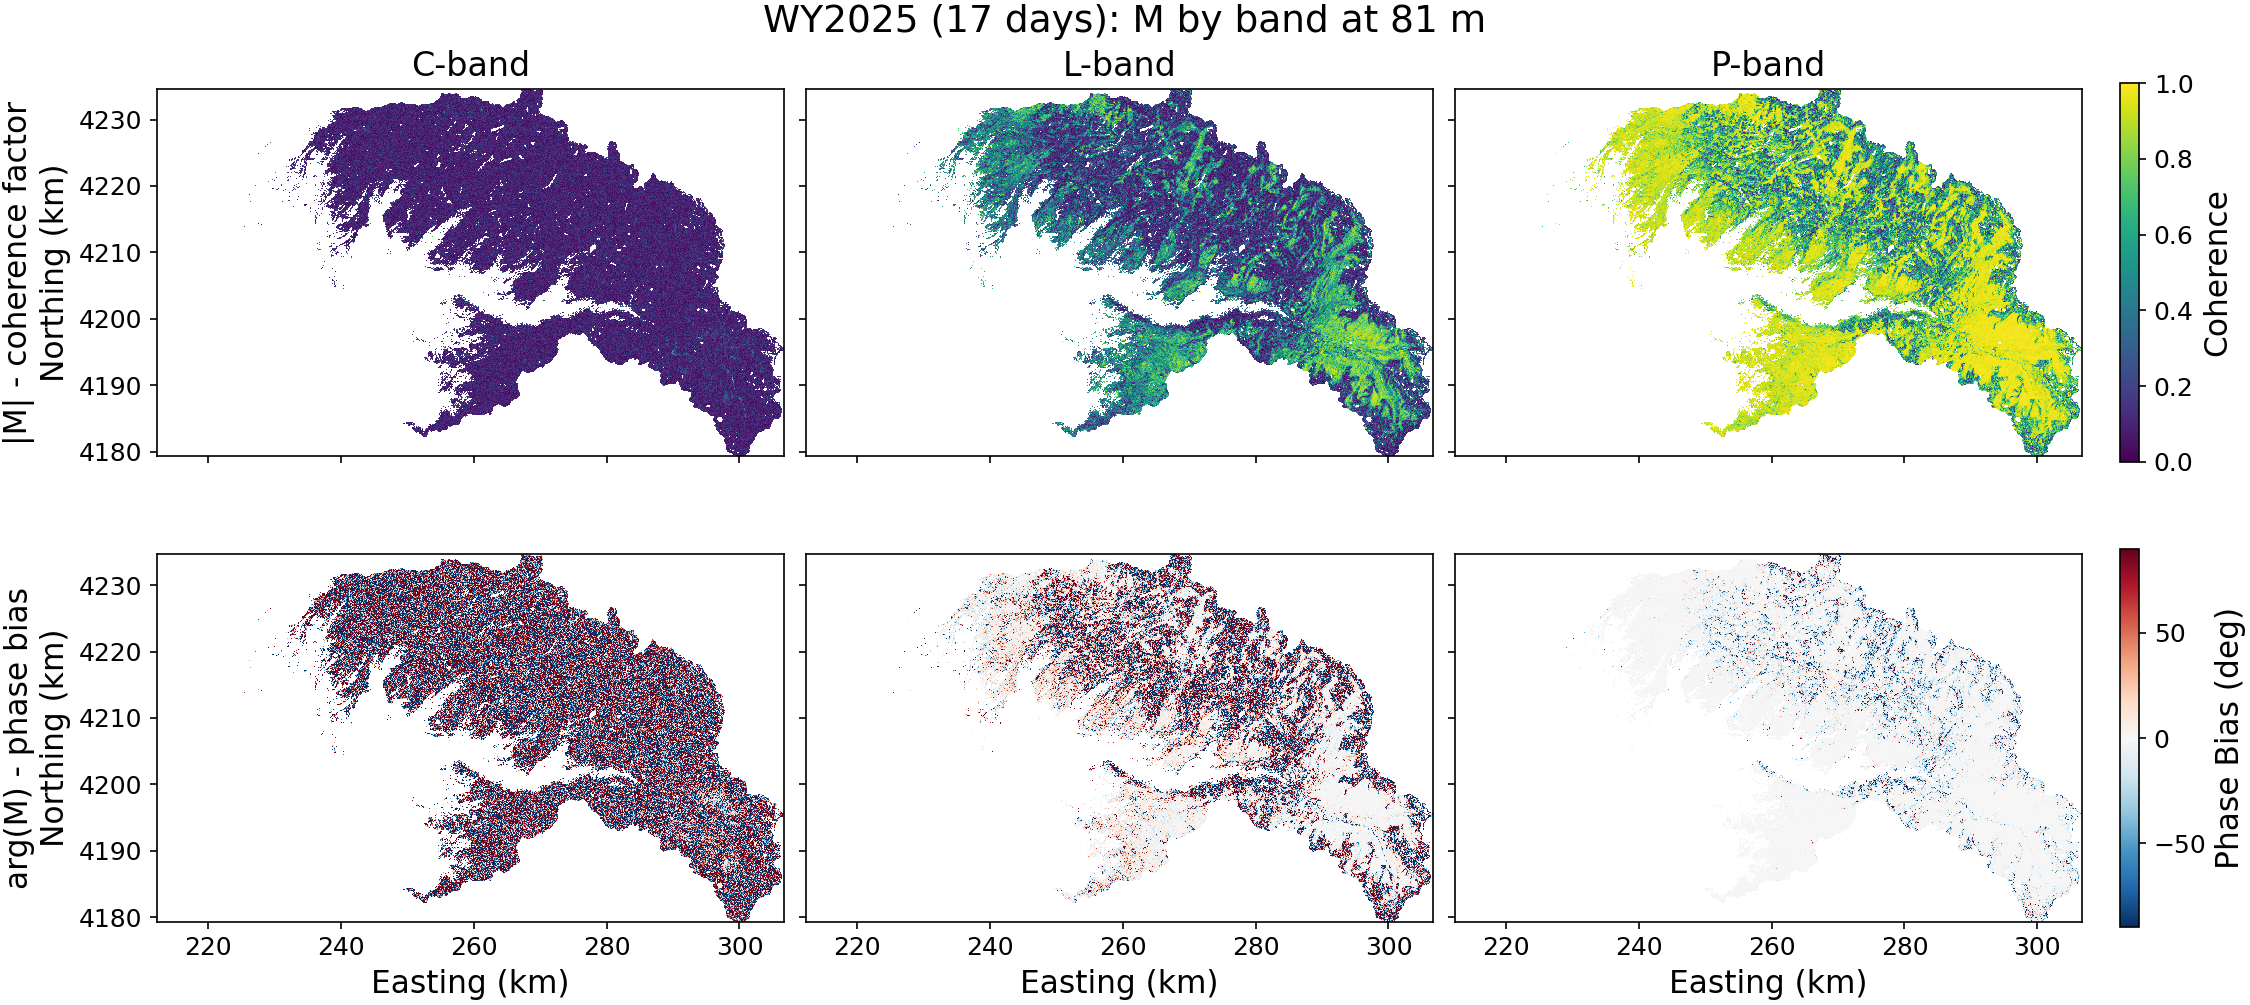
\includegraphics[width=1.0\linewidth]{figures/7_bands_M_WY2025.png}
  \caption{\DIFdelbeginFL \DIFdelFL{Sub-window coherence }\DIFdelendFL \DIFaddbeginFL \DIFaddFL{Coherence }\DIFaddendFL factor $|M|$ (\textbf{top}) and retrieval bias $\arg(M)$ (\textbf{bottom}) at 81\,\unit{m} for the WY2025 lidar pair (February 8--25, 2025) at C-, L-, and P-band.}
  \label{fig:M_bands_wy2025}
\end{figure}


\section{Discussion}\label{sec:discussion}

Using repeat lidar surveys and NISAR \DIFdelbegin \DIFdel{interferometry, we have shown that }\DIFdelend \DIFaddbegin \DIFadd{interferometric pairs, we explore how }\DIFaddend within-window $\Delta\mathrm{SWE}$ variability reduces \DIFdelbegin \DIFdel{coherence and $\Delta\mathrm{SWE}$ skew }\DIFdelend \DIFaddbegin \DIFadd{the estimated coherence and, for asymmetric distributions, }\DIFaddend biases the retrieved $\Delta\mathrm{SWE}$\DIFdelbegin \DIFdel{from the true mean $\Delta\mathrm{SWE}$, both of which degrade InSAR SWE retrievals}\DIFdelend . Here we consider what these results mean in practice: the length scales at which the $\Delta\mathrm{SWE}$ field is organized, the \DIFdelbegin \DIFdel{resulting effects at NISAR's standard postings}\DIFdelend \DIFaddbegin \DIFadd{impacts on processing specifically for SWE retrievals}\DIFaddend , and how the effect scales from C- to P-band.

\subsection{$\Delta\mathrm{SWE}$ Structure and the Processing Window Size}\label{subsec:break-discussion}

The $\Delta\mathrm{SWE}$ spectral break at $\ell_b \approx 25$\,\unit{m} (Figure~\ref{fig:psd_break}) falls within the 15--40\,\unit{m} variogram range scale breaks reported for cumulative snow depth and matches the wind- and vegetation-controlled short-scale regime of \citet{trujillo2007topographic-0ec}\DIFaddbegin \DIFadd{, and the 10 to 30\,}\unit{m} \DIFadd{snow-depth correlation lengths that \mbox{%DIFAUXCMD
\citet{yueh2026interferometric-3ba} }\hskip0pt%DIFAUXCMD
measure from lidar at Grand Mesa, Colorado}\DIFaddend . The change in SWE between two flights is therefore organized at the same length scales as the snowpack itself, so differencing two snow surfaces preserves the fine-scale structure. This holds in all four winters, so the variability driving within-window phase spread is a persistent feature of accumulation, not an artifact of a single season.

This break sets the window sizes over which the \DIFdelbegin \DIFdel{sub-window }\DIFdelend \DIFaddbegin \DIFadd{within-window }\DIFaddend coherence loss develops. Because the $\Delta\mathrm{SWE}$ field carries increasing variance toward larger scales (Section~\ref{subsec:power_spectral_densities}), the within-window phase spread keeps growing as the \DIFdelbegin \DIFdel{footprint }\DIFdelend \DIFaddbegin \DIFadd{window }\DIFaddend expands past $\ell_b$, and the coherence factor falls steadily across the GUNW range. The window-size sweep shows this in $|M|$ directly (Figure~\ref{fig:window_size}). The empirical curve is steepest below about 25\,\unit{m} and flattens beyond, with the slope change near the spectral break\DIFdelbegin \DIFdel{--- a flattening driven by }\DIFdelend \DIFaddbegin \DIFadd{. The flattening comes from }\DIFaddend $|M|$ approaching its floor once the within-window phase spread exceeds about one radian. Even in this regime the recoverable coherence is substantial: moving from the 80\,\unit{m} \DIFdelbegin \DIFdel{GUNW posting to a }\DIFdelend \DIFaddbegin \DIFadd{to the }\DIFaddend 20\,\unit{m} \DIFdelbegin \DIFdel{footprint }\DIFdelend \DIFaddbegin \DIFadd{window }\DIFaddend nearly doubles the median $|M|$, from 0.18 to 0.33. The coherence recovered per step keeps growing as the window shrinks toward $\ell_b$, so even modest reductions below the GUNW default return usable coherence over the spatially variable snow that decorrelates the 80\,\unit{m} product.

The bias result is promising for SWE retrievals. Across the full 9 to 81\,\unit{m} range, the SWE-equivalent bias in usable windows stays at the millimeter level (Figure~\ref{fig:window_size}, right), far below the coherence loss and below the retrieval uncertainty from other sources. The \DIFdelbegin \DIFdel{footprint is therefore }\DIFdelend \DIFaddbegin \DIFadd{window size is }\DIFaddend a coherence tradeoff and not a bias tradeoff. A larger window loses coherence without incurring a meaningful retrieval bias in the pixels that survive a coherence threshold, and a smaller window recovers coherence without introducing bias. The \DIFdelbegin \DIFdel{footprint }\DIFdelend \DIFaddbegin \DIFadd{window size }\DIFaddend should be chosen to keep $|M|$ usable over the target snowpack, and the residual skew-driven retrieval bias can be neglected in any window that passes a coherence mask.

Shrinking the window has a limit. Smaller windows average fewer pixels, so the random phase noise that multi-looking suppresses, whose variance falls as $1/N$ with the number of looks \citep{Bamler1998}, rises as the \DIFdelbegin \DIFdel{footprint }\DIFdelend \DIFaddbegin \DIFadd{window }\DIFaddend shrinks. The best \DIFdelbegin \DIFdel{footprint }\DIFdelend \DIFaddbegin \DIFadd{window size }\DIFaddend balances the recovered \DIFdelbegin \DIFdel{sub-window }\DIFdelend \DIFaddbegin \DIFadd{within-window }\DIFaddend coherence against this estimation noise and is set by the local $\Delta\mathrm{SWE}$ correlation length, the $\ell_b \approx 25$\,\unit{m} break, rather than a fixed look count. For these Tuolumne events that balance sits well below the 80\,\unit{m} GUNW posting, and large accumulation events such as the December 2025 storm need the \DIFdelbegin \DIFdel{finest practical footprint }\DIFdelend \DIFaddbegin \DIFadd{smallest practical window }\DIFaddend to keep the \DIFdelbegin \DIFdel{sub-window }\DIFdelend \DIFaddbegin \DIFadd{within-window }\DIFaddend term in check. The most wind-exposed terrain, where short-scale variance is largest, will be challenging to recover at any \DIFdelbegin \DIFdel{footprint}\DIFdelend \DIFaddbegin \DIFadd{window size}\DIFaddend .

\subsection{Snow-based Multi-look Coherence Bias}\label{subsec:coherence-bias}

Coherence \DIFdelbegin \DIFdel{measured }\DIFdelend over seasonal snow \DIFdelbegin \DIFdel{has historically been interpreted through }\DIFdelend \DIFaddbegin \DIFadd{is usually interpreted with }\DIFaddend a decorrelation budget of temporal, geometric, SNR, and volume terms \DIFdelbegin \DIFdel{, with residual loss most often assigned to temporal decorrelation of the snowvolume \mbox{%DIFAUXCMD
\citep{Ruiz2021, Oveisgharan2024}}\hskip0pt%DIFAUXCMD
. The presented sub-window }\DIFdelend \DIFaddbegin \DIFadd{\mbox{%DIFAUXCMD
\citep{Ruiz2021, Oveisgharan2024}}\hskip0pt%DIFAUXCMD
. Within-window }\DIFaddend $\Delta\mathrm{SWE}$ \DIFdelbegin \DIFdel{effect is itself a change-driven }\DIFdelend \DIFaddbegin \DIFadd{variability has been recognized as an additional term \mbox{%DIFAUXCMD
\citep{LiSturm2002, Rott2003, ming2026, yueh2026interferometric-3ba}}\hskip0pt%DIFAUXCMD
, but its size has been inferred from interferograms or from models rather than measured from the snow. It is one component of temporal }\DIFaddend decorrelation, since it \DIFdelbegin \DIFdel{arises }\DIFdelend \DIFaddbegin \DIFadd{comes }\DIFaddend from the snow that accumulates between passes, \DIFdelbegin \DIFdel{but it differs from the usual temporal term: rather than the stochastic motion of sub-resolution }\DIFdelend \DIFaddbegin \DIFadd{alongside dielectric change, the appearance or removal of scatterers, and the random motion of }\DIFaddend scatterers within a cell\DIFdelbegin \DIFdel{, }\DIFdelend \DIFaddbegin \DIFadd{. It differs from those components in acting between cells rather than within them: }\DIFaddend it is the deterministic variation of the resolved $\Delta\mathrm{SWE}$ field across \DIFdelbegin \DIFdel{cells within }\DIFdelend \DIFaddbegin \DIFadd{the cells of }\DIFaddend the multi-look window. \DIFdelbegin \DIFdel{Our lidar-derived $|M|$ maps show that a substantial share of the L-band coherence drop over an accumulation interval may be this deterministic sub-window componentrather than stochastic temporal decorrelation. Because it is set by the resolved snow structure, it }\DIFdelend \DIFaddbegin \DIFadd{That difference matters because the within-window component, unlike the within-cell ones, }\DIFaddend can be predicted from lidar and reduced \DIFdelbegin \DIFdel{by processing at a finer footprint, neither of which is true of the stochastic temporal term to which it is usually attributed}\DIFdelend \DIFaddbegin \DIFadd{with a smaller window or other processing choices}\DIFaddend . Across the four Tuolumne lidar pairs \DIFdelbegin \DIFdel{, the sub-window factor }\DIFdelend \DIFaddbegin \DIFadd{it }\DIFaddend lowers the basin-median $|M|$ \DIFaddbegin \DIFadd{at an 81\,}\unit{m} \DIFadd{window }\DIFaddend to 0.25 \DIFdelbegin \DIFdel{--0.47 }\DIFdelend \DIFaddbegin \DIFadd{to 0.47 }\DIFaddend (Figure~\ref{fig:aso_all_pairs})\DIFdelbegin \DIFdel{at an 81\,}%DIFDELCMD < \unit{m} %%%
\DIFdel{window}\DIFdelend , a coherence loss of 0.5 to 0.75 \DIFdelbegin \DIFdel{carried by within-window $\Delta\mathrm{SWE}$ structure before any }\DIFdelend \DIFaddbegin \DIFadd{before any within-cell }\DIFaddend temporal or thermal term is applied\DIFaddbegin \DIFadd{, so much of the L-band temporal decorrelation over an accumulation interval may be this component rather than change within the cells}\DIFaddend .

\DIFdelbegin \DIFdel{Turning to the NISAR data , both the raw coherence and the multi-resolution residual }\DIFdelend \DIFaddbegin \DIFadd{The NISAR data }\DIFaddend show the temporal and spatial patterns \DIFdelbegin \DIFdel{that these lidar $\Delta\mathrm{SWE}$ results predict}\DIFdelend \DIFaddbegin \DIFadd{the lidar results predict, in both the raw coherence and the coherence difference between window sizes }\DIFaddend (Figure~\ref{fig:coherence_rows}). The raw 80\,\unit{m} coherence is lower for the December 19--31 storm pair than for the \DIFdelbegin \DIFdel{near-snow-free }\DIFdelend \DIFaddbegin \DIFadd{no-accumulation }\DIFaddend December 7--19 pair\DIFdelbegin \DIFdel{, and within }\DIFdelend \DIFaddbegin \DIFadd{. Within }\DIFaddend the storm pair it is lowest over the steep alpine terrain where \DIFdelbegin \DIFdel{sub-window }\DIFdelend \DIFaddbegin \DIFadd{within-window }\DIFaddend $\Delta\mathrm{SWE}$ variability is greatest\DIFdelbegin \DIFdel{(median $\gamma_{80}\approx0.17$ }\DIFdelend \DIFaddbegin \DIFadd{, with a median $\hat{\gamma}_{80}$ of about 0.16 }\DIFaddend at the highest elevations \DIFdelbegin \DIFdel{versus $\approx0.27$ }\DIFdelend \DIFaddbegin \DIFadd{against 0.26 }\DIFaddend at the lowest\DIFdelbegin \DIFdel{)}\DIFdelend . Raw coherence alone cannot separate the \DIFdelbegin \DIFdel{sub-window }\DIFdelend \DIFaddbegin \DIFadd{within-window }\DIFaddend loss from other decorrelation\DIFdelbegin \DIFdel{, but the corrected $\gamma_{20}-\gamma_{80}$ residual repeats both patterns where only the sub-window }\DIFdelend \DIFaddbegin \DIFadd{. The corrected residual $\tilde{\gamma}_{20}-\tilde{\gamma}_{80}$, in which only the within-window }\DIFaddend term should appear\DIFdelbegin \DIFdel{. It is }\DIFdelend \DIFaddbegin \DIFadd{, repeats both patterns: }\DIFaddend near zero for the no-accumulation pair (median $-0.004$), positive for the storm pair (median \DIFdelbegin \DIFdel{$+0.030$ }\DIFdelend \DIFaddbegin \DIFadd{$+0.028$ }\DIFaddend over snow), and largest in the highest, most complex terrain (90th percentile \DIFdelbegin \DIFdel{$\Delta \gamma$ 0.13}\DIFdelend \DIFaddbegin \DIFadd{0.12}\DIFaddend ). The \DIFdelbegin \DIFdel{observed }\DIFdelend residual is smaller than the lidar-predicted gap \DIFdelbegin \DIFdel{($|M|_{20}-|M|_{80}\approx0.15$, }\DIFdelend \DIFaddbegin \DIFadd{of about 0.15 (}\DIFaddend Section~\ref{subsec:window-size-results}) because $\gamma_\mathrm{other}$ multiplies the difference and much of the storm-pair scene is decorrelated enough that the gap is lost to phase noise. \DIFdelbegin \DIFdel{Coherence over snow may therefore be misattributed to temporal decorrelation when part of it is a }\DIFdelend \DIFaddbegin \DIFadd{That the residual follows the predicted pattern supports the presence of the }\DIFaddend within-window \DIFdelbegin \DIFdel{phase-variability signal}\DIFdelend \DIFaddbegin \DIFadd{term in real data and shows that comparing coherence across window sizes can identify it}\DIFaddend .

Even \DIFdelbegin \DIFdel{at a finer footprint}\DIFdelend \DIFaddbegin \DIFadd{with a smaller window}\DIFaddend , the retrieval is more tractable where the $\Delta\mathrm{SWE}$ field is smooth. The $|M|$ drops to 0.12--0.16 in the steep, wind-exposed alpine drainages but stays near one over the lower-elevation, gently varying terrain (Figure~\ref{fig:aso_all_pairs}, center column). This terrain control holds across events. The basin-median $\Delta\mathrm{SWE}$ for our four pairs spans an order of magnitude, while the median $|M|$ stays within a narrow band, so the decorrelation and bias are set by terrain and snowpack structure rather than by event size. Since some multi-looking will be necessary to improve phase estimates, retrievals will work best when targeted at regions and snowpacks whose $\Delta\mathrm{SWE}$ varies gently relative to the multi-look window. \DIFdelbegin \DIFdel{The }\DIFdelend \DIFaddbegin \DIFadd{In the }\DIFaddend most variable alpine terrain \DIFdelbegin \DIFdel{may be unrecoverable at any current spaceborne footprint}\DIFdelend \DIFaddbegin \DIFadd{the within-window spread stays large even at the 20\,}\unit{m} \DIFadd{window, where a quarter of all windows still have $|M|$ below 0.2 (Figure~\ref{fig:window_size}), so those areas may not be recoverable at the window sizes of current spaceborne products}\DIFaddend .

Melt periods may be more favorable than accumulation for the \DIFdelbegin \DIFdel{sub-window }\DIFdelend \DIFaddbegin \DIFadd{within-window }\DIFaddend term considered here. Once the snowpack has ripened and refrozen, melt-driven $\Delta\mathrm{SWE}$ varies smoothly with elevation and aspect rather than in wind-built drifts, which keeps the within-window variance and skew low. The WY2023 melt-versus-accumulation split (Section~\ref{subsec:lidar-variability}) shows this directly, with the gap persisting at matched $|\Delta\mathrm{SWE}|$ magnitude and driven by a lower within-window spread, so melt removes SWE more uniformly within the window than wind deposits it. This smoother \DIFdelbegin \DIFdel{sub-window }\DIFdelend \DIFaddbegin \DIFadd{within-window }\DIFaddend signal only helps if the wet-snow dielectric and temporal decorrelation terms in $\gamma_\mathrm{other}$ do not collapse the coherence on their own. L-band ablation retrievals have been initially demonstrated for morning refrozen acquisitions \citep{Tarricone2023}, but they will be sensitive to the estimated liquid water content, as this impacts the radar wave speed and, therefore, the phase.

\DIFdelbegin \DIFdel{This mechanism also explains why wind }\DIFdelend \DIFaddbegin \DIFadd{Wind }\DIFaddend is the single largest control on snow coherence in \DIFdelbegin \DIFdel{\mbox{%DIFAUXCMD
\citet{Ruiz2022}}\hskip0pt%DIFAUXCMD
. }\DIFdelend \DIFaddbegin \DIFadd{the tower observations of \mbox{%DIFAUXCMD
\citet{Ruiz2022}}\hskip0pt%DIFAUXCMD
. The area a tower images is smaller than a satellite resolution cell, so there the redistribution acts within the cell, the sub-cell path-length spread of \mbox{%DIFAUXCMD
\citet{Rott2003}}\hskip0pt%DIFAUXCMD
, rather than across a multi-look window. The mechanism is the same phase spread at a smaller scale. }\DIFaddend Wind is the main \DIFdelbegin \DIFdel{agent }\DIFdelend \DIFaddbegin \DIFadd{cause }\DIFaddend of fine-scale snow redistribution, building dunes, scour, and drifts at length scales well below typical multi-look window sizes \citep{trujillo2007topographic-0ec}. This redistribution raises the within-window $\Delta\mathrm{SWE}$ variance and skew, which shortens and rotates $M$, so a windy interval produces the asymmetric, \DIFdelbegin \DIFdel{sub-window }\DIFdelend \DIFaddbegin \DIFadd{within-window }\DIFaddend $\Delta\mathrm{SWE}$ distribution that Figure~\ref{fig:theoretical_example} identifies as the source of both coherence loss and retrieval bias. This is the same mechanism \citet{LiSturm2002} identified at C-band, where mapped ERS-1 coherence loss tracked the spatial and temporal patterns of wind-driven redistribution, and that \citet{ming2026} found for C-band over first-year sea ice by decomposing the coherence budget. Our results \DIFdelbegin \DIFdel{confirm }\DIFdelend \DIFaddbegin \DIFadd{support }\DIFaddend both findings from lidar rather than from the interferograms themselves. At C-band, the wavelength examined by \citet{LiSturm2002} and \citet{ming2026}, $|M|$ collapses to a median of 0.10, and the lowest $|M|$ in every pair falls in the wind-exposed alpine terrain.
\DIFdelbegin \DIFdel{The dominance of wind as a predictor in \mbox{%DIFAUXCMD
\citet{Ruiz2022} }\hskip0pt%DIFAUXCMD
is what we would expect if sub-window $\Delta\mathrm{SWE}$ variability, rather than bulk temporal changes affecting temporal coherence, governs the observed coherence.
}\DIFdelend 

\subsection{Skew-Driven Retrieval Bias Considerations}\label{subsec:phase-bias}

The sign of the retrieval bias \DIFaddbegin \DIFadd{$\arg(M)$ }\DIFaddend is set by the skew of the within-window $\Delta\mathrm{SWE}$ distribution (Figure~\ref{fig:theoretical_example}). Before the phase wraps, a positively skewed distribution produces a negative retrieval bias, which rotates the multi-looked phase below the true window-mean phase and results in a lower retrieved $\Delta\mathrm{SWE}$ than the true mean in those windows. A physically likely source of this positive skew is wind loading: a few wind-loaded pixels carry much more new snow than the rest of the window and sit as positive outliers in an otherwise smooth $\Delta\mathrm{SWE}$ field, lengthening the right tail of the distribution.

The \DIFdelbegin \DIFdel{lidar-derived $\arg(M)$ }\DIFdelend \DIFaddbegin \DIFadd{lidar-predicted retrieval bias }\DIFaddend maps show the \DIFdelbegin \DIFdel{same pattern }\DIFdelend \DIFaddbegin \DIFadd{largest bias in wind-exposed terrain }\DIFaddend (Figure~\ref{fig:aso_all_pairs}, right column). The \DIFdelbegin \DIFdel{retrieval bias is a real effect, but it is a small one. It is }\DIFdelend \DIFaddbegin \DIFadd{bias is }\DIFaddend near zero across most of the basin and rises only in the steep, wind-exposed alpine terrain, where the within-window variability is largest and the coherence is lowest. This $\Delta\mathrm{SWE}$ bias is \DIFdelbegin \DIFdel{therefore largest exactly }\DIFdelend \DIFaddbegin \DIFadd{largest }\DIFaddend where the phase is least reliable. In SWE terms, it stays near $\pm5$\,\unit{mm} (converting phase to L-band $\Delta\mathrm{SWE}$ bias) across the basin and reaches about 1.5\,\unit{cm} only in the most wind-affected windows of the largest event. Because the bias peaks with the coherence loss, pixels that pass a coherence threshold carry little bias, so it mostly affects pixels that may already be unusable. This coupling \DIFdelbegin \DIFdel{only holds at shorter wavelengths}\DIFdelend \DIFaddbegin \DIFadd{holds at L-band and shorter wavelengths because the same within-window phase spread that produces the bias also removes the coherence}\DIFaddend . At longer wavelengths \DIFdelbegin \DIFdel{, }\DIFdelend \DIFaddbegin \DIFadd{the smaller $\kappa$ keeps that spread small, so }\DIFaddend the coherence is preserved while the \DIFaddbegin \DIFadd{skew-driven }\DIFaddend bias remains, which we turn to below.

\subsection{C-, L-, and P-band Analysis}\label{subsec:band-analysis}

P-band is appealing for SWE retrieval. The smaller $\kappa$ keeps coherence high over the large accumulation events that decorrelate L-band. However, at P-band, the retrieval bias is still present and consistently negative ($\arg(M)$ IQR $-1.6^\circ$ to $+0.3^\circ$), and it is the one band where the bias is not correlated with almost complete coherence drops. The negative sign is the one predicted for a positively skewed $\Delta\mathrm{SWE}$ distribution, and it appears here because the longer wavelength keeps the within-window phase spread small enough that the multi-looked phase does not wrap (Figure~\ref{fig:phase_wraps_bands}). At C- and L-band, the same bias is present but masked since the larger phase spread wraps and pulls the median $\arg(M)$ back toward zero. A longer-wavelength sensor has a narrower window phase distribution, but where the distribution is skewed in the steep alpine terrain, it carries a systematic negative bias without the matching total coherence loss to flag it.

Shorter wavelengths run into the opposite problem. At C-band, the within-window phase variability is large enough that the coherence collapses, with a pooled median $|M|$ of 0.10 and more than half of the WY2025 windows below 0.1 (Figure~\ref{fig:M_bands_wy2025}). A C-band sensor recovers little usable $\Delta\mathrm{SWE}$ over snow at this multi-look window size (81\,\unit{m}). \DIFdelbegin %DIFDELCMD < 

%DIFDELCMD < %%%
\DIFdel{This collapse is dominated by the real sub-window $\Delta\mathrm{SWE}$ structure, but because independent decorrelation sources multiply, some component is likely lidar depth noise.That noise component is accentuated at C-band, where the larger $\kappa$ turns the same residual depth error into a much larger phase spread than at L-band (further discussed in Appendix~\ref{appendix:noise}}\DIFdelend \DIFaddbegin \DIFadd{By Eq.~(\ref{eq:cumulant}), C-band keeps a coherence factor above 0.3 only where the within-window $\Delta\mathrm{SWE}$ spread stays below about 0.7\,}\unit{cm}\DIFadd{, against a median of 3.4\,}\unit{cm} \DIFadd{in the Tuolumne storm windows. The C-band retrievals reported to date \mbox{%DIFAUXCMD
\citep{Oveisgharan2024, oveisgharan2025using-92d, bovenga2025multi-band-f90} }\hskip0pt%DIFAUXCMD
were made in snow climates with smaller accumulations than the Tuolumne storms, and our result implies that within-window variability would prevent C-band retrieval of major accumulation events in complex terrain. Future work will test how commonly this within-window variability prevents C-band retrievals (Section~\ref{subsec:mitigation}}\DIFaddend ).

%DIF >  This collapse is dominated by the real within-window $\Delta\mathrm{SWE}$ structure, but because independent decorrelation sources multiply, some component is likely lidar depth noise. That noise component is accentuated at C-band, where the larger $\kappa$ turns the same residual depth error into a much larger phase spread than at L-band (further discussed in Appendix~\ref{appendix:noise}).
\DIFaddbegin 

\DIFaddend L-band falls between the two. The pooled median $|M|$ of 0.33 leaves enough coherence to recover phase over the smoother, lower-elevation terrain but not over the steep alpine drainages, where $|M|$ drops toward the C-band regime. The bias is likewise intermediate and only partly wrapped ($\arg(M)$ IQR $-15^\circ$ to $+19^\circ$). L-band \DIFdelbegin \DIFdel{, therefore, escapes the coherence collapse that overwhelms }\DIFdelend \DIFaddbegin \DIFadd{is less affected by coherence loss than }\DIFaddend C-band, and, unlike P-band, its retrieval bias is paired with a coincident coherence loss that will cause those pixels with bias to be removed anyway.

\subsection{Mitigation and Future Work}\label{subsec:mitigation}

The \DIFdelbegin \DIFdel{multi-resolution comparison }\DIFdelend \DIFaddbegin \DIFadd{comparison across window sizes }\DIFaddend used here is itself a potential mitigation. The coherence loss due to \DIFdelbegin \DIFdel{sub-window }\DIFdelend \DIFaddbegin \DIFadd{within-window }\DIFaddend $\Delta\mathrm{SWE}$ variability grows with window size\DIFaddbegin \DIFadd{, }\DIFaddend while the other decorrelation terms do not\DIFdelbegin \DIFdel{, so }\DIFdelend \DIFaddbegin \DIFadd{. Therefore, }\DIFaddend comparing corrected coherence across \DIFdelbegin \DIFdel{footprints separates the sub-window }\DIFdelend \DIFaddbegin \DIFadd{window sizes separates the within-window }\DIFaddend contribution from the rest, and the \DIFdelbegin \DIFdel{$\gamma_{20}-\gamma_{80}$ }\DIFdelend \DIFaddbegin \DIFadd{$\tilde{\gamma}_{20}-\tilde{\gamma}_{80}$ }\DIFaddend residual is a direct, if noisy, estimate of $1-|M|$ that could flag windows where \DIFdelbegin \DIFdel{sub-window }\DIFdelend \DIFaddbegin \DIFadd{within-window }\DIFaddend variability dominates. The limit is that even the 20\,\unit{m} window sits well inside the variability regime for large storms, so \DIFdelbegin \DIFdel{two GUNW resolutions }\DIFdelend \DIFaddbegin \DIFadd{the two GUNW window sizes }\DIFaddend sample only part of the $|M|$ curve (Figure~\ref{fig:window_size}) \DIFdelbegin \DIFdel{, and pixels that are fully decorrelated at both footprints remain unrecoverable}\DIFdelend \DIFaddbegin \DIFadd{and pixels decorrelated by other sources make the estimate noisy}\DIFaddend .

Processing \DIFdelbegin \DIFdel{at a finer posting }\DIFdelend \DIFaddbegin \DIFadd{with a smaller window }\DIFaddend reduces both the \DIFdelbegin \DIFdel{sub-window }\DIFdelend \DIFaddbegin \DIFadd{within-window }\DIFaddend coherence loss and the retrieval bias but increases the random phase noise as each window averages fewer pixels. Phase linking, which estimates a consistent phase time series from all interferometric pairs in an acquisition stack \DIFdelbegin \DIFdel{to reduce phase noise}\DIFdelend \DIFaddbegin \DIFadd{\mbox{%DIFAUXCMD
\citep{Guarnieri2008, ansari2017sequential-aff, eppler2022adapting-c4d, zwieback2022cheap-026}}\hskip0pt%DIFAUXCMD
}\DIFaddend , could offset this\DIFdelbegin \DIFdel{by averaging over time rather than space, using temporal averaging instead of spatial multi-looking to achieve reasonable phase estimates \mbox{%DIFAUXCMD
\citep{Guarnieri2008, ansari2017sequential-aff, eppler2022adapting-c4d, zwieback2022cheap-026}}\hskip0pt%DIFAUXCMD
}\DIFdelend \DIFaddbegin \DIFadd{. It still forms the coherence by spatial averaging, but the redundancy of the many pairs in the stack acts as additional looks, so a smaller multi-look window can reach the same phase noise}\DIFaddend . This route needs testing on real data. Processing a NISAR stack well below the 80\,\unit{m} GUNW posting and phase linking across acquisitions would show whether the recovered $\Delta\mathrm{SWE}$ improves over the standard product. It only helps where the scene remains coherent across the stack, so it favors slowly evolving snowpacks over the windy, rapidly redistributing terrain that drives the largest losses.

Triplet closure phases may identify and mitigate variability-induced bias of the phase-based SWE estimator. The closure phase\DIFdelbegin \DIFdel{$\Phi_{123}=\arg(z_{12}z_{23}z_{13}^{*})$
}\DIFdelend \DIFaddbegin \DIFadd{, the sum of the interferometric phases around a triplet of acquisitions, }\DIFaddend is insensitive to any phase that separates into per-acquisition terms, such as the tropospheric or mean SWE phase, thus isolating the non-separable $\arg(M)$ term \citep{zwieback2024temporal-426}. The confounding factor is that the closure signal is both largest and noisiest for large $\Delta\mathrm{SWE}$ variability and, thus, low coherence, and that soil-moisture and wet-snow dielectric changes produce their own non-zero closure that must be separated from the \DIFdelbegin \DIFdel{sub-window }\DIFdelend \DIFaddbegin \DIFadd{within-window }\DIFaddend term \citep{Zan2014, zwieback2016statistical-d35}.

The clearest next step is to apply the same $|M|$ and $\arg(M)$ pipeline to lidar pairs in other basins and snow climates. Repeating it across maritime, continental, and tundra snowpacks would map where the \DIFdelbegin \DIFdel{sub-window }\DIFdelend \DIFaddbegin \DIFadd{within-window }\DIFaddend effect is severe and tie the coherence loss to a measurable property of each site, such as the $\Delta\mathrm{SWE}$ break scale, rather than to a single basin. A NISAR acquisition coincident with a lidar pair would close the remaining gap by directly testing whether the lidar-predicted \DIFdelbegin \DIFdel{sub-window }\DIFdelend \DIFaddbegin \DIFadd{within-window }\DIFaddend loss matches the observed \DIFdelbegin \DIFdel{$\gamma_{20}-\gamma_{80}$ }\DIFdelend \DIFaddbegin \DIFadd{$\tilde{\gamma}_{20}-\tilde{\gamma}_{80}$ }\DIFaddend residual, rather than relying on the consistency in sign shown here.

\subsection{Limitations}\label{subsec:limitations}

This analysis has several limitations. The conversion from lidar $\Delta H_{\mathrm{snow}}$ to $\Delta\mathrm{SWE}$ uses a single basin-constant snow density for the new accumulated snow for each pair rather than a spatially varying one, \DIFdelbegin \DIFdel{which, in reality, will be more spatially variable than bulk density}\DIFdelend \DIFaddbegin \DIFadd{although the density of new snow varies more in space than the bulk density does}\DIFaddend . We made this choice because ASO provides density only at a 50\,\unit{m} resolution, and it has minimal impact on the results. Using a spatially variable density shifts the basin-median $|M|$ by at most 0.03 and leaves the per-window $|M|$ tightly correlated with the constant-density value (Pearson $r = 0.91$ to $0.98$ across the four pairs). The basin-median $\arg(M)$ moves by less than $2^\circ$. A constant density also matters mainly when the density itself varies within the window. If the denser wind slabs coincide with the deep, drift-loaded pixels, the true $\Delta\mathrm{SWE}$ outliers are larger than estimated, so the constant-density assumption most likely understates the within-window variance and skew and is conservative for the effect reported here.

The analysis also covers a single basin and four lidar pairs. The \DIFdelbegin \DIFdel{sub-window }\DIFdelend \DIFaddbegin \DIFadd{within-window }\DIFaddend effect depends on the spatial structure of $\Delta\mathrm{SWE}$, which varies with storm patterns, climate, terrain, and snowpack regimes. \DIFdelbegin \DIFdel{Therefore, the }\DIFdelend \DIFaddbegin \DIFadd{The }\DIFaddend $|M|$ and $\arg(M)$ magnitudes here should not be interpreted as representative of all snow types. Shallower or more uniform snowpacks would show smaller coherence decreases and retrieval bias, while wind-dominated tundra could show as much or more. Confirming the size of the effect elsewhere requires comparable lidar pairs in other regions.

The NISAR coherence and the lidar $\Delta\mathrm{SWE}$ fields are also not from the same dates. The \DIFdelbegin \DIFdel{multi-resolution coherence }\DIFdelend \DIFaddbegin \DIFadd{NISAR coherence comparison }\DIFaddend comes from December 2025 acquisitions with no coincident flights, while the $|M|$ maps come from lidar pairs in other years. The comparison \DIFdelbegin \DIFdel{, therefore, }\DIFdelend tests only the general spatial and temporal trends between the accumulation and no-accumulation NISAR pairs and cannot directly confirm that a given coherence drop comes from the \DIFdelbegin \DIFdel{sub-window }\DIFdelend \DIFaddbegin \DIFadd{within-window }\DIFaddend variability of that same scene. It assumes the spatial $\Delta\mathrm{SWE}$ pattern on the NISAR accumulation pair dates resembles the $\Delta\mathrm{SWE}$ pattern from the lidar pairs used to predict $|M|$, which holds only to the extent that the terrain-driven accumulation structure repeats between events. Paired lidar flights coincident with both NISAR observations forming an interferogram would be necessary to fully attribute the coherence drop to the \DIFdelbegin \DIFdel{sub-window }\DIFdelend \DIFaddbegin \DIFadd{within-window }\DIFaddend $\Delta\mathrm{SWE}$ variability.

Both $|M|$ and $\arg(M)$ here assume that every per-cell phasor has unit amplitude. Real backscatter differs between pixels with different physical properties, such as soil moisture, roughness, and rock and vegetation cover of the ground surface beneath the snow. If these amplitude differences correlate with the same outlier pixels that drive the skew, they would amplify or dampen the bias relative to this unit-amplitude estimate.

\DIFaddbegin \DIFadd{The constant 40$^{\circ}$ incidence angle likewise excludes within-window variation of $\kappa$ with terrain. At L-band $\kappa$ changes by about 0.7\,}\unit{rad\,m^{-1}} \DIFadd{per degree of incidence angle, so a $\pm5^{\circ}$ spread of local incidence angle within a window holding 10\,}\unit{cm} \DIFadd{of $\Delta\mathrm{SWE}$ adds a phase spread of $\pm0.3$\,}\unit{rad} \DIFadd{even where the $\Delta\mathrm{SWE}$ is uniform, against the 1 to 2\,}\unit{rad} \DIFadd{spread the $\Delta\mathrm{SWE}$ variability itself produces in a typical window. Over steep terrain this incidence-angle variation changes the within-window phase spread, but by much less than the $\Delta\mathrm{SWE}$ variability does. Whether it widens or narrows the spread depends on the correlation between the local incidence angle and snow accumulation.
}

\DIFaddend A remaining concern is that part of the $|M|$ drop could be lidar depth noise rather than \DIFdelbegin \DIFdel{sub-window }\DIFdelend \DIFaddbegin \DIFadd{within-window }\DIFaddend $\Delta\mathrm{SWE}$ structure, since any residual per-pixel depth error adds its own within-window phase spread. We bound this two ways in Appendix~\ref{appendix:noise}. At L- and P-band, the noise-only $|M|$ is 0.96 and 1.00 against observed medians of 0.33 and 0.88, so depth noise accounts for almost none of the loss. C-band is the tightest case: its noise floor of about 0.45 is the only one that removes a large share of the coherence on its own, but since the factors multiply, the observed collapse to 0.10 still requires real $\Delta\mathrm{SWE}$ structure to dominate. Even so, the C-band $|M|$ should be treated as a conservative lower bound, given the larger noise contribution.

Finally, the Tuolumne pairs were flown by ASO to bracket the dominant winter storm events. These large accumulations, combined with the spatially complex alpine terrain, maximize the within-window variance. \DIFdelbegin \DIFdel{Therefore, the }\DIFdelend \DIFaddbegin \DIFadd{The }\DIFaddend coherence losses reported here for the storm pairs are likely an upper bound on the problem rather than a typical value over a winter time series. Smaller events, mid-elevation terrain, and slowly varying melt will likely \DIFdelbegin \DIFdel{be above these }\DIFdelend \DIFaddbegin \DIFadd{have higher }\DIFaddend $|M|$ \DIFdelbegin \DIFdel{values}\DIFdelend \DIFaddbegin \DIFadd{than reported here}\DIFaddend .

\conclusions  %% \conclusions[modified heading if necessary]
We use repeat lidar to predict, independently of any radar observations, how the spatial variability of the $\Delta\mathrm{SWE}$ field drives an apparent loss of InSAR coherence, separate from the \DIFaddbegin \DIFadd{within-cell }\DIFaddend temporal, geometric, and thermal decorrelation\DIFdelbegin \DIFdel{that is usually considered for coherence over snow}\DIFdelend . We also show that the skew of that within-window $\Delta\mathrm{SWE}$ variability biases the retrieved $\Delta\mathrm{SWE}$, though this effect is negligible compared to the decorrelation at L-band. Over four Tuolumne lidar pairs, this \DIFdelbegin \DIFdel{sub-window }\DIFdelend \DIFaddbegin \DIFadd{within-window }\DIFaddend variability alone lowers the L-band coherence factor $|M|$ to a basin median of 0.25 to 0.47, a coherence loss carried entirely by within-window $\Delta\mathrm{SWE}$ structure, and adds a per-window retrieval bias of a few millimeters of SWE that reaches about 1.5\,\unit{cm} in the steep alpine terrain. We use two NISAR pairs, one spanning a large storm and one with little snow change, to show that the observed coherence and its change with \DIFdelbegin \DIFdel{resolution }\DIFdelend \DIFaddbegin \DIFadd{window size }\DIFaddend are spatially and temporally consistent with this \DIFdelbegin \DIFdel{sub-window }\DIFdelend \DIFaddbegin \DIFadd{within-window }\DIFaddend loss.

The $\Delta\mathrm{SWE}$ field is organized around a measurable length scale. Its power spectrum has a scale break at $\ell_b \approx 25$\,\unit{m}, the same fine-scale roughness break reported for snow depth in previous studies, and sweeping the multi-look window across this scale shows the median coherence factor falling from 0.54 at 9\,\unit{m} to 0.18 at 81\,\unit{m}, with most of the loss incurred by a few tens of meters. Moving from the 80\,\unit{m} \DIFdelbegin \DIFdel{GUNW posting to a }\DIFdelend \DIFaddbegin \DIFadd{to the }\DIFaddend 20\,\unit{m} \DIFdelbegin \DIFdel{footprint }\DIFdelend \DIFaddbegin \DIFadd{window }\DIFaddend nearly doubles the median coherence factor at L-band, from 0.18 to 0.33, while the skew-driven retrieval bias remains at the millimeter level at every \DIFdelbegin \DIFdel{footprint}\DIFdelend \DIFaddbegin \DIFadd{window size}\DIFaddend .

The effect scales strongly with wavelength. At C-band, the within-window phase spread collapses the coherence (median $|M|$ of 0.10) and leaves almost no recoverable phase, while P-band preserves the coherence (median 0.88) but still carries a small systematic negative retrieval bias. For L-band \DIFdelbegin \DIFdel{, }\DIFdelend NISAR, this means that coherence \DIFaddbegin \DIFadd{loss }\DIFaddend over spatially variable snow should not be \DIFdelbegin \DIFdel{considered as temporal decorrelation }\DIFdelend \DIFaddbegin \DIFadd{attributed to change within the resolution cells }\DIFaddend alone, and that large accumulation events need processing at finer scales than the standard 80\,\unit{m} GUNW posting to be effectively recovered. More broadly, the within-window structure of $\Delta\mathrm{SWE}$ sets a sampling limit on any \DIFdelbegin \DIFdel{fixed-footprint }\DIFdelend \DIFaddbegin \DIFadd{fixed-window }\DIFaddend InSAR SWE retrieval. Because that limit is set by the snow and not the sensor, it can be predicted and accommodated through the choice of \DIFdelbegin \DIFdel{processing resolution}\DIFdelend \DIFaddbegin \DIFadd{window size}\DIFaddend , wavelength, and timing, rather than appearing as \DIFdelbegin \DIFdel{unexplained and }\DIFdelend unrecoverable coherence loss.


%% The following commands are for the statements about the availability of data sets and/or software code corresponding to the manuscript.
%% It is strongly recommended to make use of these sections in case data sets and/or software code have been part of your research the article is based on.

% \codeavailability{TEXT} %% use this section when having only software code available


% \dataavailability{TEXT} %% use this section when having only data sets available


\codedataavailability{All processing and analysis code is available at \url{https://github.com/zachhoppinen/tc_snow_variability_insar}. Airborne Snow Observatory (ASO) lidar snow depth and SWE products are available through the ASO data portal (\url{https://data.airbornesnowobservatories.com/}). The NISAR geocoded unwrapped interferogram (GUNW) products are available from the Alaska Satellite Facility (\url{https://search.asf.alaska.edu/}).}

% \sampleavailability{TEXT} %% use this section when having geoscientific samples available


% \videosupplement{TEXT} %% use this section when having video supplements available


\appendix
\section{Lidar Noise Limitation}\label{appendix:noise}    %% Appendix A

This appendix bounds the contribution of lidar depth noise to $|M|$. Because the $|M|$ calculation runs on the 9\,\unit{m} block-averaged $\Delta\mathrm{SWE}$ field, any residual per-pixel depth error adds its own within-window phase spread, which could appear as \DIFdelbegin \DIFdel{sub-window }\DIFdelend \DIFaddbegin \DIFadd{within-window }\DIFaddend $\Delta\mathrm{SWE}$ structure. We bound this noise in two independent ways.

First, the radial power spectrum of the 3\,\unit{m} $\Delta\mathrm{SWE}$ field is a clean fractal power law with no flat high-frequency shelf from spatially uncorrelated noise, which rules out the large per-pixel noise that would otherwise appear as such a shelf. The high-frequency tail bounds the per-pixel 3\,\unit{m} noise at about 1.7\,\unit{cm} of SWE, or 0.5\,\unit{cm} per 9\,\unit{m} cell after the block average. Second, the $\Delta\mathrm{SWE}$ over snow-free bare ground, where the true change is zero, is random per-pixel speckle of comparable magnitude (about 1.6\,\unit{cm} at 3\,\unit{m} for WY2025). On the 9\,\unit{m} working grid, both estimates give a noise-only $|M|$ of about 0.45 at C-band, 0.96 at L-band, and 1.00 at P-band, against observed medians of 0.10, 0.33, and 0.88. At L- and P-band, the noise factor is near one, so depth noise accounts for almost none of the loss. Because the noise and $\Delta\mathrm{SWE}$-structure factors multiply, C-band is the tightest case: a 0.45 noise floor still leaves the observed 0.10 requiring a real \DIFdelbegin \DIFdel{sub-window }\DIFdelend \DIFaddbegin \DIFadd{within-window }\DIFaddend factor near 0.2, so structure dominates over noise at every band.

These same bounds explain our processing choices. This per-pixel noise is why the main pipeline pre-averages to 9\,\unit{m} before forming $M$. \DIFdelbegin \DIFdel{At }\DIFdelend \DIFaddbegin \DIFadd{On }\DIFaddend the native 3\,\unit{m} \DIFdelbegin \DIFdel{posting}\DIFdelend \DIFaddbegin \DIFadd{grid}\DIFaddend , the same bounds imply a noise-only $|M|$ near 0.67 at L-band, which the 3$\times$3 block average suppresses to 0.96. The window-size sweep (Section~\ref{subsec:window-size-results}) must run on the native 3\,\unit{m} field to resolve its smallest windows, so its $|M|$ curve carries this noise. Because the per-pixel noise is spatially uncorrelated, its contribution to $M$ is a window-size-independent multiplicative factor, so the shape of the curve, the location of its scale break, and the ratio between \DIFdelbegin \DIFdel{footprints are unaffected; only }\DIFdelend \DIFaddbegin \DIFadd{window sizes are unaffected. Only }\DIFaddend the absolute level is deflated, which is why the sweep $|M|$ is reported as a lower bound.

\section{VIIRS Snow-Cover Cross-Check}\label{appendix:viirs}    %% Appendix B
\appendixfigures
\DIFdelbegin %DIFDELCMD < \appendixfigures
%DIFDELCMD < %%%
\DIFdel{The corrected multi-resolution residual $\gamma_{20}-\gamma_{80}$ }\DIFdelend \DIFaddbegin \DIFadd{The corrected coherence difference between window sizes $\tilde{\gamma}_{20}-\tilde{\gamma}_{80}$ }\DIFaddend (Section~\ref{subsec:nisar-coherence}) attributes the storm-pair coherence drop to within-window $\Delta\mathrm{SWE}$ variability. As an independent check that this signal tracks snow, rather than a bare-ground or vegetation artifact, we compare it against optical snow cover.

We use the VIIRS daily cloud-gap-filled NDSI snow-cover product VNP10A1F, Version 2 (Suomi-NPP VIIRS, 375\,\unit{m} sinusoidal grid, tile h08v05\DIFdelbegin \DIFdel{; }\DIFdelend \DIFaddbegin \DIFadd{, }\DIFaddend distributed by the NSIDC DAAC) \citep{riggs2022vnp10a1f}. The cloud-gap-filled layer carries each cell forward from its most recent clear observation, so every NISAR pair window has continuous coverage. For each NISAR pair we pull the product on the end date of its temporal baseline (December 19, 2025 for the no-accumulation pair P12 and December 31, 2025 for the storm pair P23), because the decorrelation in an accumulation pair is driven by the new snow, which is only fully on the ground at the end of the baseline. We convert the NDSI snow cover (0--100) to fractional snow-covered area (fSCA) via the linear relation $\mathrm{fSCA} = -0.01 + 1.45\,(\mathrm{NDSI}/100)$, clipped to $[0,1]$ \citep{salomonson2004}, and reproject it (nearest neighbor) onto the same 81\,\unit{m} grid and WY2023 \DIFdelbegin \DIFdel{footprint }\DIFdelend \DIFaddbegin \DIFadd{extent }\DIFaddend used for the coherence panels in Figure~\ref{fig:coherence_rows}. Figure~\ref{fig:viirs} places the per-pair fSCA beside the corrected \DIFdelbegin \DIFdel{$\gamma_{20}-\gamma_{80}$ }\DIFdelend \DIFaddbegin \DIFadd{$\tilde{\gamma}_{20}-\tilde{\gamma}_{80}$ }\DIFaddend for the same pair.

Within the surveyed \DIFdelbegin \DIFdel{footprint}\DIFdelend \DIFaddbegin \DIFadd{extent}\DIFaddend , the fSCA increases with elevation toward the high alpine terrain where the storm-pair residual is largest. Across \DIFdelbegin \DIFdel{the footprint the }\DIFdelend \DIFaddbegin \DIFadd{that extent the }\DIFaddend corrected residual co-varies with fSCA for the storm pair (Pearson \DIFdelbegin \DIFdel{$r=+0.40$, Spearman $\rho=+0.43$; }\DIFdelend \DIFaddbegin \DIFadd{$r=+0.39$ and Spearman $\rho=+0.41$, with }\DIFaddend mean fSCA 0.58 \DIFdelbegin \DIFdel{, median residual $+0.015$}\DIFdelend \DIFaddbegin \DIFadd{and median residual $+0.013$}\DIFaddend ) and only weakly for the no-accumulation pair (Pearson \DIFdelbegin \DIFdel{$r=+0.08$, Spearman $\rho=+0.09$; }\DIFdelend \DIFaddbegin \DIFadd{$r=+0.09$ and Spearman $\rho=+0.10$, with }\DIFaddend mean fSCA 0.12 \DIFdelbegin \DIFdel{, median residual $-0.005$}\DIFdelend \DIFaddbegin \DIFadd{and median residual $-0.006$}\DIFaddend ). The correlation is moderate by construction since fSCA indicates where snow lies rather than how much $\Delta\mathrm{SWE}$ accumulated, which is the quantity that drives the \DIFdelbegin \DIFdel{sub-window }\DIFdelend \DIFaddbegin \DIFadd{within-window }\DIFaddend decorrelation.

\begin{figure}
\centering
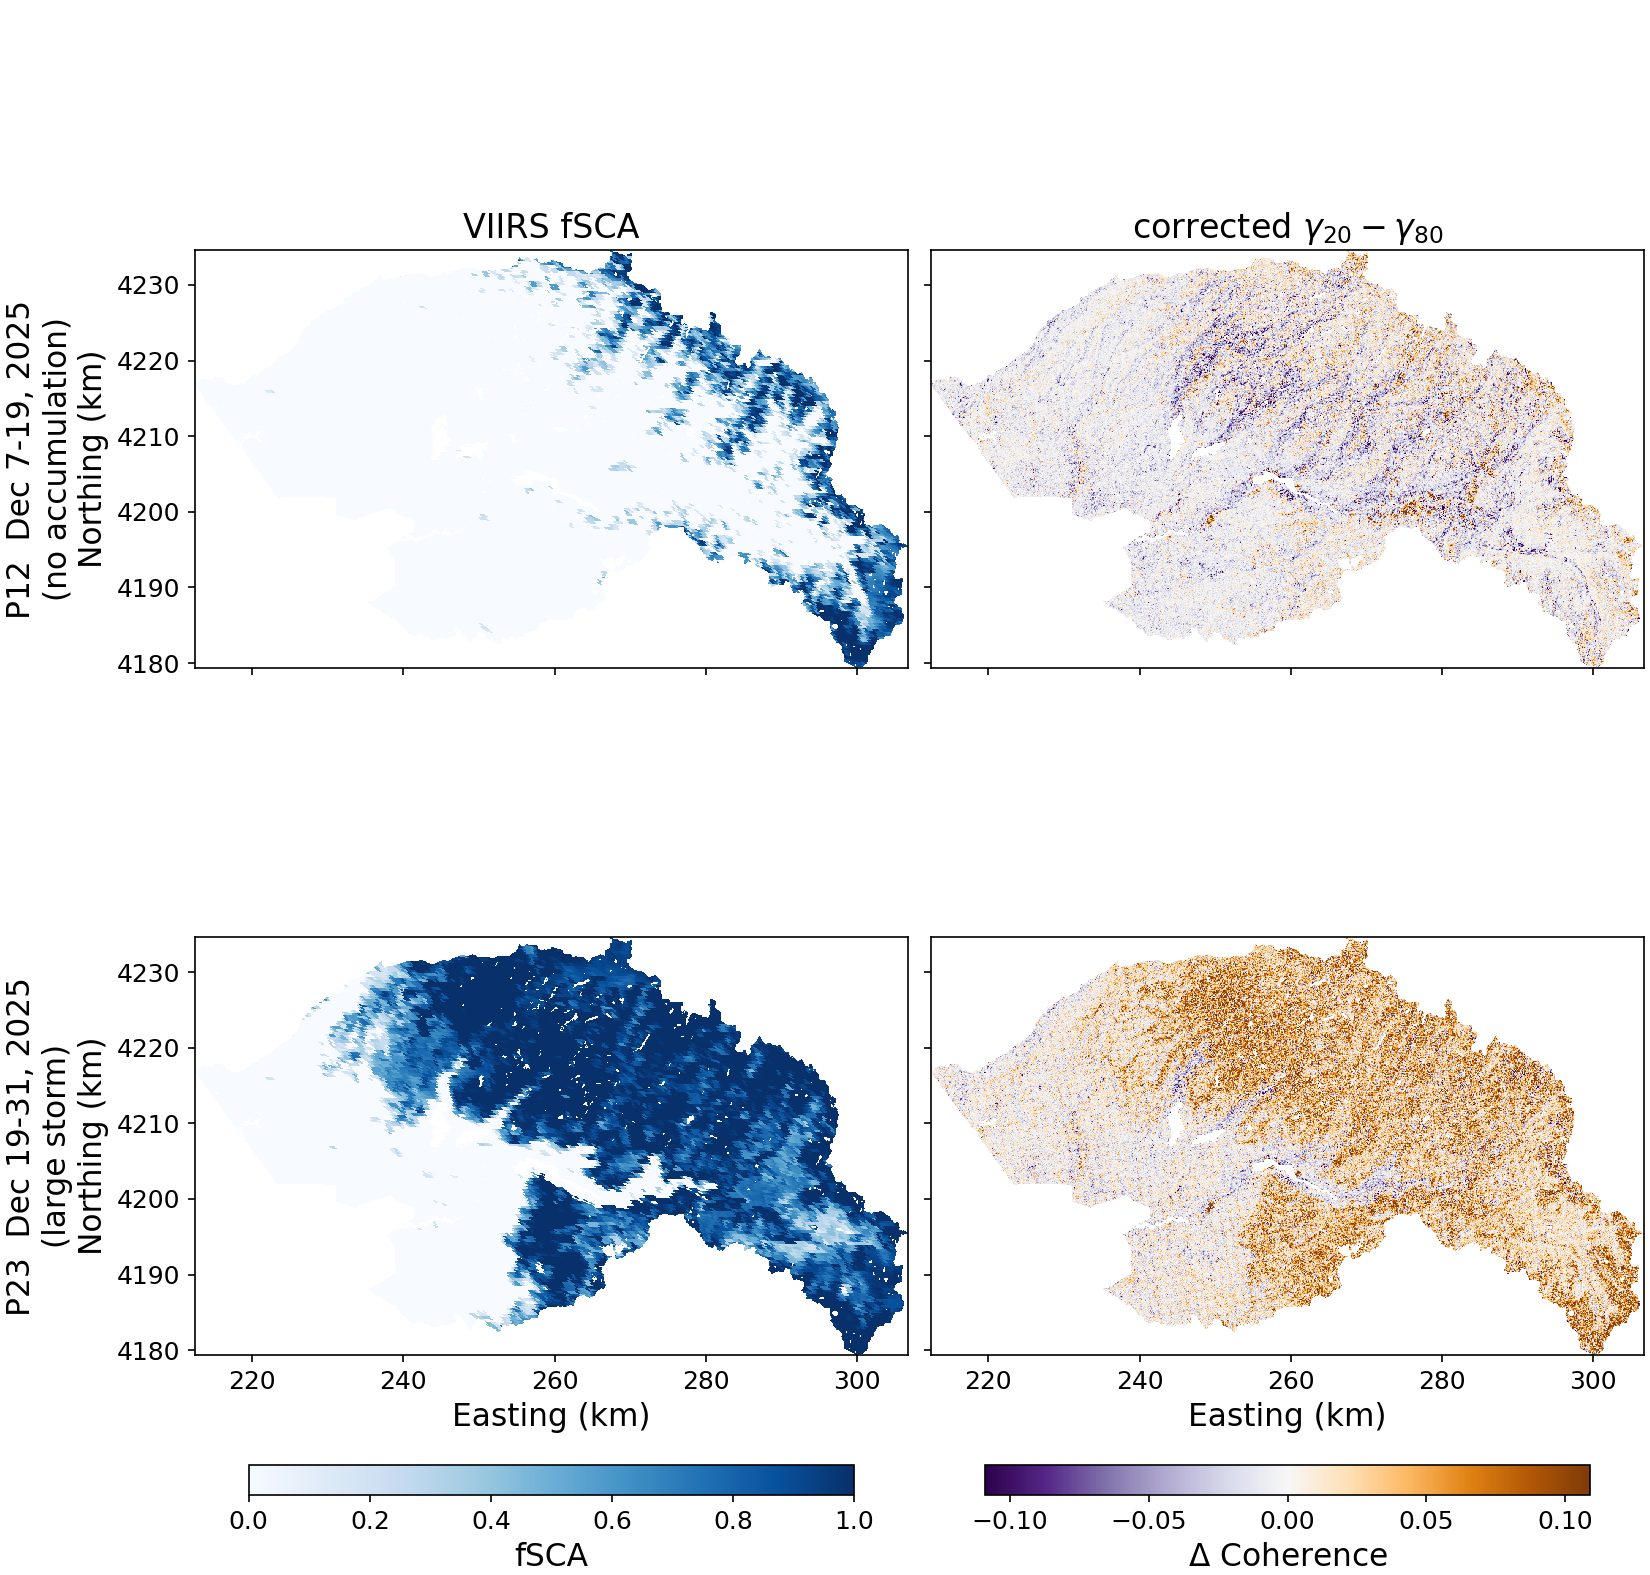
\includegraphics[width=\linewidth]{figures/B1_snowcover_vs_dgamma.png}
  \caption{VIIRS VNP10A1F fractional snow-covered area (fSCA) (\textbf{left}) and the corrected \DIFdelbeginFL \DIFdelFL{$\gamma_{20}-\gamma_{80}$ }\DIFdelendFL \DIFaddbeginFL \DIFaddFL{$\tilde{\gamma}_{20}-\tilde{\gamma}_{80}$ }\DIFaddendFL residual (\textbf{right}) for the no-accumulation P12 pair (\textbf{top}) and the large-storm P23 pair (\textbf{bottom}), on each pair's end date and shown on the common WY2023 81\,\unit{m} \DIFdelbeginFL \DIFdelFL{footprint}\DIFdelendFL \DIFaddbeginFL \DIFaddFL{extent}\DIFaddendFL . The storm-pair residual is largest over the high-elevation terrain where fSCA is highest.}
  \label{fig:viirs}
\end{figure}

\noappendix       %% use this to mark the end of the appendix section. Otherwise the figures might be numbered incorrectly (e.g. 10 instead of 1).

%% Regarding figures and tables in appendices, the following two options are possible depending on your general handling of figures and tables in the manuscript environment:

%% Option 1: If you sorted all figures and tables into the sections of the text, please also sort the appendix figures and appendix tables into the respective appendix sections.
%% They will be correctly named automatically.

%% Option 2: If you put all figures after the reference list, please insert appendix tables and figures after the normal tables and figures.
%% To rename them correctly to A1, A2, etc., please add the following commands in front of them:

% \appendixfigures  %% needs to be added in front of appendix figures

% \appendixtables   %% needs to be added in front of appendix tables

%% Please add \clearpage between each table and/or figure. Further guidelines on figures and tables can be found below.
\FloatBarrier


\authorcontribution{ZH conceived the study, developed the methodology, carried out the analysis, and wrote the original manuscript. SZ contributed to the conceptual development of the study and reviewed and edited the manuscript. RP and HPM reviewed and edited the manuscript. All authors read and approved the final manuscript.} %% this section is mandatory

\competinginterests{The authors declare that they have no competing interests.} %% this section is mandatory even if you declare that no competing interests are present

% \disclaimer{TEXT} %% optional section

\begin{acknowledgements}
These ASO data were paid for by California Department of Water Resources and Turlock Irrigation District in the nominal operational program.

This work utilized \DIFdelbegin \DIFdel{pre-calibration (Beta) }\DIFdelend \DIFaddbegin \DIFadd{provisional }\DIFaddend data (https://doi.org/10.5067/\DIFdelbegin \DIFdel{NIL1GUNW-B1}\DIFdelend \DIFaddbegin \DIFadd{NIL2GUNW-P1}\DIFaddend ) made available by the NASA-ISRO SAR (NISAR) mission, obtained from the Alaska Satellite Facility DAAC.

This work was supported by NASA grants 80NSSC25K7452 (ZH, RP, HPM), 80NSSC24K1082 (RP) and 80NSSC25K7386 (SZ).

The authors used Anthropic's Claude (via Claude Code) to assist with figure-generation code and manuscript text editing.
\end{acknowledgements}

%% REFERENCES
%% Since the Copernicus LaTeX package includes the BibTeX style file copernicus.bst,
%% authors experienced with BibTeX only have to include the following two lines:
%%
\bibliographystyle{copernicus}
\bibliography{references.bib,references2.bib}

\end{document}
